\documentclass[acmsmall,review,anonymous]{acmart}\settopmatter{printfolios=true,printccs=false,printacmref=false}
\usepackage{amsmath}
% \usepackage{theorem}
\usepackage{proof}
% \usepackage{macros}
\usepackage{graphicx}
\usepackage{xspace}
\usepackage[all]{xy}
\usepackage{macros}
\usepackage{ebproof}
\usepackage{stmaryrd}
\usepackage{rotating,color,xcolor}
\usepackage{tikz}
\usetikzlibrary{automata, positioning, arrows}
\begin{document}
 \title{First-order tree-to-tree functions}
 \author{Amina and Mikolaj}
 \maketitle

%  \tableofcontents

\section{Introduction}

The purpose of this paper is to decompose tree transformations into simple building blocks. An important inspiration  is the Krohn-Rhodes theorem~\cite[p.~454]{Krohn1965}, which says that every string-to-string function recognised by a Mealy machine can be decomposed into certain prime functions. 

\paragraph*{Regular functions.} The transformations studied in this paper are the so called  regular functions.

In~\cite[Theorem 13]{engelfrietMSODefinableString2001}, Engelfriet and Hoogeboom proved that deterministic two-way transducers recognise the same string-to-string functions as \mso transductions. Because of this and other properties -- such as closure under composition~\cite[Theorem 1]{chytilSerialComposition2Way1977} and decidable equivalence~\cite[Theorem 1]{gurariEquivalenceProblemDeterministic1982} --  this class of functions is now called the \emph{regular string-to-string functions}. Other  equivalent descriptions of the regular functions include: string transducers of Alur and {\v C}ern{\'y}~\cite{alurExpressivenessStreamingString2010}, and several models based on combinators~\cite{alur2014regular,daveGastinKrishna18, bojanczykRegularFirstOrderList2018}. 
 
% One corollary of the description in~\cite{bojanczykRegularFirstOrderList2018} is that the regular  string-to-string functions are the smallest class of string-to-string functions which is closed under composition, contains functions recognised by one-way deterministic automata, and the following two operations:
% \begin{eqnarray*}
% w_1 |  \cdots | w_n &\qquad \mapsto \qquad& w_1 w_1 |  \cdots | w_n w_n, \\
% w_1 |  \cdots | w_n &\qquad \mapsto \qquad& \text{reverse}(w_1) |  \cdots | \text{reverse}(w_n),
% \end{eqnarray*}
% where $w_1,\ldots,w_n \in \set{a,b}^*$ and $|$ is a separator symbol. The deterministic one-way automata themselves can be further decomposed using the Krohn-Rhodes theorem; thus leading a decomposition into very simple prime functions.

There are also regular functions for trees, which can be defined using any of the following equivalent models: \mso tree-to-tree transductions~\cite[Section 3]{bloem_comparison_2000}, single use attributed tree grammars~\cite{bloem_comparison_2000}, macro tree transducers of linear size increase~\cite[Theorem 7.1]{engelfriet_macro_2003}, and streaming tree transducers~\cite[Theorem 4.6]{alur2017streaming}. 

The goal of this paper is to prove a decomposition result for regular tree-to-tree functions. As in the Krohn-Rhodes theorem, we want to show that every such function can be obtained by combining certain prime functions.  

\paragraph*{First-order transductions. } Although \mso transductions are the more popular model, we work mainly with the less expressive model of first-order transductions. Why?

As we explain in Section~\ref{sec:mso-trans}, every \mso tree-to-tree transduction can be decomposed as: (a) first, a relabelling defined in \mso, which does not change the tree structure; followed by (b) a first-order tree-to-tree transduction. In this sense, as far as transformations of the tree structure are concerned,  first-order and \mso transductions have the same expressive power. Another argument for the importance of first-order tree-to-tree transductions is the connection with the $\lambda$-calculus. As we explain in Section~\ref{sec:stt-derivable}, first-order tree-to-tree transductions are expressive enough to capture evaluation of $\lambda$-terms (which are linear, i.e.~every variable is used once), and such evaluation turns out to be one of the core computational steps implicit in a tree-to-tree transduction. 

Another advantage of first-order logic on trees is that it has a better decomposition theory, in the sense of decomposing formulas into combinations of simpler ones~\cite{haferthomas,bojanczykDecidablePropertiesTree2004,esik-weil1}. 
% This theory includes characterisations in terms of the temporal logic {\sc ctl*} \cite[Main Theorem]{haferthomas}, cascade products of tree automata~\cite[Theorem 2.5.7]{bojanczykDecidablePropertiesTree2004}, block products~\cite[Corollary 3.11]{esik2010algebraic} and wreath products~\cite[Theorem 3.1]{bojanczykWreathProductsForest2012}. 
For our paper, the most useful decomposition is a remarkable theorem of Schlingloff, which shows that first-order logic on trees is equivalent to a certain two-way variant  {\sc ctl}~\cite[Theorem 4.5]{schlingloff1992expressive}. In contrast, there are no such results for \mso. 
% One reason is that \mso on trees is too hard if we are interested in Krohn-Rhodes decompositions.  Already for the simplest tree formalisms, such as tree languages or letter-to-letter transformations, there is no known  Krohn-Rhodes theory. One would expect a Krohn-Rhodes theorem  for trees to yield an effective characterisation of first-order logic -- as it does for words -- but finding such a characterisation remains a major open problem~\cite[Section 3]{bojanczyk2015automata}. We do not attempt to solve this problem here. In contrast, first-order logic on trees does have decomposition theorems, which we can use: including

% Another, more positive, reason is that in terms of restructuring trees, first-order logic is not that far from \mso.  By~\cite[Corollary 1]{colcombetCombinatorialTheoremTrees2007},  every \mso tree-to-tree transduction can be decomposed into an \mso transduction that does not change the tree structure, followed by a first-order transduction. Furthermore, as we show in this paper, first-order logic is sufficient for certain fundamental transformations, such as evaluating $\lambda$-terms. 


Summing up, we believe that first-order  tree transformations are an expressive model, with a strong theory, and deserve to leave the shadow of their better known \mso cousin.


\paragraph*{Structured datatypes.} We present our main decomposition result using a formalism based on  functional programming (in a combinatory variant, i.e.~without variables), with structured datatypes such as pairs or co-pairs.  The motivation behind this approach  -- which is inspired by~\cite{bojanczykRegularFirstOrderList2018} -- is that we want to avoid syntactic annotation with endmarkers and separators that typically appears when working with Krohn-Rhodes decompositions. Thanks to the  structured datatypes,  we can use established operations such as {\tt map}. Also, we can assign informative types to our functions, such as $\Sigma_1 \times \Sigma_2 \to \Sigma_i$ for projection, as opposed to saying that all functions input and output trees.  The choice of datatypes for trees is harder than for the string case that was studied in~\cite{bojanczykRegularFirstOrderList2018}.  The difficulty is in splitting the input into smaller pieces. A piece of a string is also a string, but this is no longer true for trees, where the pieces have dangling edges (or variables). As a result, more complicated  datatypes are needed; and our design choices lead us to functions that operate on ranked sets, where each element has an associated arity.
 


This is a long paper. Given the limited space, we have decided to prioritise  explaining  design choices and intuitions, with  examples and many pictures. As a result, almost all of the proofs are in the appendix. 




\section{Trees and tree-to-tree functions}
\label{sec:trees-transductions}
 In this section, we describe the trees and tree-to-tree functions that are discussed in this paper. The  trees are rooted, node labelled, ranked (the label of a node determines the number of children) and sibling ordered (there is a first child, second child, etc.). 
A \emph{ranked set} is a set where each element has an associated \emph{arity} in $\set{0,1,2,\ldots}$. We adopt the convention that ranked sets are written in red, e.g.~$\rSigma$ or $\rGamma$.  We use ranked sets as building blocks for trees. The following picture describes the notion of trees that we use and some terminology:\\

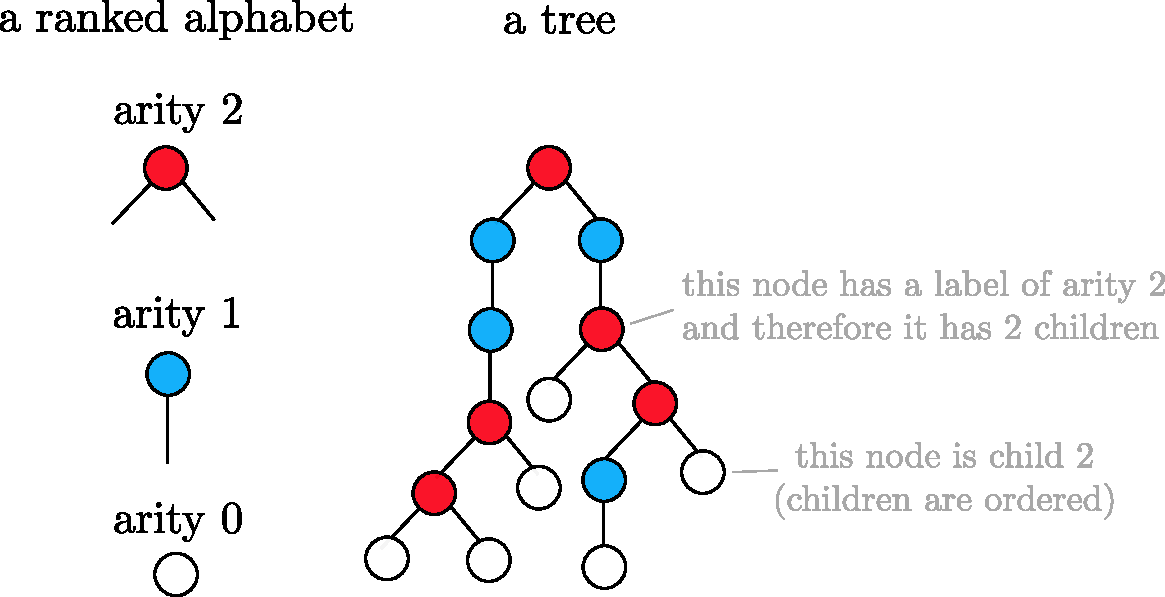
\includegraphics[scale=.4]{ranked-tree.pdf}

% When talking about elements of a ranked set, we mean elements of the underlying set.   For a ranked set $A$ and a finite set of variables $X \subseteq \varnames$, we write $\slice A X$ for the elements of $A$ that have arity $X$. 

We use standard tree terminology, such as ancestor, descendant, child, parent. We write $\trees \rSigma$ for the set of trees over a ranked set $\rSigma$. This paper is about \emph{tree-to-tree functions}, which are functions of the type \begin{align*}
f : \trees \rSigma \to \trees \rGamma.
\end{align*}
We also discuss tree languages, i.e.~sets of trees. 
A tree language can be viewed as the special case of a tree-to-tree function, where the output alphabet $\Gamma$ contains only two letters ``yes'' and ``no'' of arity zero. Later on, we will also discuss terms, which are trees with variables. 

  
\subsection{First-order logic and transductions}
In this section we  describe how logics -- such as first-order logic or monadic second-order logic -- can be used to define tree-to-tree functions and tree languages. The basic idea is to view a tree as a model, and to use logic to describe properties and transformations of such models\footnote{For more about these logics in the context of defining properties of trees, see~\cite[Section 3]{thomas1997languages}.}. 

A \emph{relational vocabulary} is defined to be a set of relation names, each one with associated arity (we do not use function symbols in this paper). Formally speaking, a relational vocabulary is the same as a ranked set, which is why we write relational vocabularies in red, using letters like $\ranked \sigma, \ranked \tau$. 

\begin{definition}[Tree as a model]\label{def:tree-model}
   For a tree $t$  over a ranked alphabet $\rSigma$, its \emph{associated model} $\underline t$ is defined as follows. The  universe is the nodes of the tree, and it is equipped with the following predicates:
   $$\begin{array}{lcl}
   x<y & : &   \text{$x$ is an ancestor of $y$} \\
   \mathrm{child}_i(x) & : & \text{$x$ is an $i$-th child (for each $i\in \set{1,2,\ldots}$)} \\
   a(x) & : &   \text{$x$ has label $a$ (for each $a \in \Sigma$)}
   \end{array}$$
    \end{definition}

The $i$-th child predicates are only needed for $i$ up to the maximal arity letters in the ranked alphabet, and hence the vocabulary in the above definition is finite. 
 A sentence of first-order logic (or of \mso)  over this vocabulary   describes a tree language, namely the set of trees whose associated models satisfy the sentence.  For example, the sentence 
 \begin{align*}
 \forall x \ a(x) \Rightarrow \exists y \ x < y \land b(x)
 \end{align*} 
 is true in (the models associated to)  trees $t$ where every node with label $a$ has a descendant with label $b$.  
 
 \paragraph*{Tree-to-tree functions.}
 Apart from defining yes/no properties, first-order logic can also be used  to define transformations on  models. In the context of this paper, we are interested in first-order transductions%\footnote{   First-order transductions are  a special case of a first-order interpretations~\cite[p.~213]{hodges_model_1993}, which use tuples (instead of elements) in the input structure to describe elements in the output structure. As a result, first-order transductions have linear size increase, while first-order interpretations have polynomial size increase. First-order transductions are also a special case of \mso transductions, see~\cite[Section 7]{courcelle_graph_2012}, which use \mso logic instead of first-order logic, and which also allow a step where the input structure is nondeterministically coloured (and therefore the result is a binary relation on structures which is not necessarily functional).}
, defined below. 

\begin{definition}[First-order transduction]\label{def:fo-transduction}\ 
\begin{enumerate}
    \item \emph{Copying.} Fix some  relational vocabulary $\ranked \sigma$ and let $k \in \set{1,2,\ldots}$. Define $k$-copying to be the operation 
    $$\begin{array}{lll}
     \text{models over $\ranked \sigma$} & \to & 
     \begin{array}{c}
     \text{models over $\ranked \sigma$}\\ 
     \text{extended with a $k$-ary relation $\mathrm{copy}$}
     \end{array}
    \end{array}$$
which inputs a model $\mathbb A$, and outputs $k$ disjoint copies of $\mathbb A$, where the  $\mathrm{copy}$ relation is interpreted as the set of tuples $(a_1,\ldots,a_k)$ such that, for  some $a \in \mathbb A$, the first copy of $a$ is  $a_1$, the second copy of $a$ is $a_2$, etc. The $\mathrm{copy}$ relation  is not commutative, because we distinguish the copies.
\item    \emph{Non-copying first-order transduction.} The syntax of a \emph{non-copying first-order transduction}  is given by:
\begin{enumerate}
    \item Input relational vocabulary $\ranked\sigma$ and output relational vocalbulary $\ranked{\gamma}$.
    \item A first-order \emph{universe formula} $\varphi(x)$ over $\ranked{\sigma}$.
    \item For every relation $R$ in vacubulary $\ranked{\gamma}$, a first-order  formula $\varphi_R(x_1,\ldots,x_{\arity R})$ over $\ranked{\sigma}$.
\end{enumerate}
The semantics of a non-copying first-order transduction is  a function
\begin{align*}
    \text{models over $\ranked\sigma$} \quad \to \quad \text{models over $\ranked\gamma$}
\end{align*}
defined as follows. If the input model is $\mathbb A$, then the output model is defined as follows: the universe is elements of $\mathbb A$ which satisfy the universe formula, and each relation $R$ is interpreted as those tuples that satisfy $\varphi_R$. 
\item \emph{First-order transductions.} A \emph{first-order transduction} is defined to be any  composition of $k$-copying (for some $k$) followed by a non-copying first-order transduction. 
 \end{enumerate}
\end{definition}



Every first-order  transduction has linear size increase, i.e.~if the input structure has a finite universe of size $n$, then the output structure has a universe of size at most $kn$, where $k$ is the number of copies used in the transduction. First-order transductions are easily seen to be closed under composition.

\begin{definition}[First-order tree-to-tree transduction.]
    A \emph{first-order tree-to-tree transduction} is any tree-to-tree  function which can be implemented by a first-order transduction, assuming that trees are modelled according to Definition~\ref{def:tree-model}. More formally, a first-order tree-to-tree transduction is any function $f$ which makes the following diagram commute
    \begin{align*}
        \xymatrix{
            \trees \rSigma \ar[d]_{t \mapsto \underline t}\ar[r]^f & \trees \rGamma \ar[d]^{t \mapsto \underline t} \\
            \set{\underline t : t \in \trees \rSigma} \ar[r]_g & \set{\underline t : t \in \trees \rGamma}.
        } 
    \end{align*}
for some first-order transduction $g$.     
\end{definition}


There are also \mso tree-to-tree transductions, these will be discussed later, in Section~\ref{sec:mso-trans}.  We conclude this section with an example of first-order tree-to-tree transduction. A more elaborated example could be found in Appendix~\ref{sec:appendix-example-fo-transductions}.

\begin{example}
    Let the input and output alphabets be:
    \mypic{17}
    and consider the tree-to-tree function which removes the unary nodes:
\mypic{19}
This is a first-order tree-to-tree transduction, which needs no copying (formally speaking, it uses 1-copying). The domain formula selects nodes which have non-unary labels, and the descendant relation is inherited from the input tree. To define the child relation on the output tree, we need to use the descendant relation in the input tree. A node $x$ in the input tree is an $i$-th child in the output tree if it satisfies the following first-order formula:
\begin{align*}
    \exists y \ \child i (y) \land \underbrace{y \le x \land   \forall z\ (y < z < x \Rightarrow \blueball(z))}_{\substack{\text{$y$ is the farthest ancestor that can be} \\ \text{reached from $x$ using only unary nodes}}}
\end{align*}
This function could not be implemented by a first-order transduction if we replaced the descendant relation by a binary parent-child relation.
\end{example}


\section{Derivable functions}
In this section, we state the main result of this paper, which describes  the  first-order tree-to-tree functions in terms of  certain atomic functions by using certain combinators.  A typical combinator is composition of functions.

\paragraph*{The category of ranked sets.} Even if our goal is to generate first-order tree-to-tree transductions, our basic functions will not necessarily be function transforming trees into trees. For example, we will need to manipulate pairs of trees or trees of trees etc. Clearly, these data structures are encodable by trees, however this would make the basic functions rather complex. We make the choice of introducing new types for our basic functions in order to get simple basic functions.

Among the types that we introduce, the most important one is certainly the type of \emph{terms}. This type appears when we want to decompose our trees into smaller parts, as illustrated by the figure below. Each small part of the tree is not really a tree\footnote{This is a difference of trees as opposed to strings~\cite{bojanczykRegularFirstOrderList2018}, where ranked sets are not needed, because a part of a string is also a string.}: it has dangling ports which  allows to connect it with the other parts. We call \emph{terms} such tree with ports. 
\mypic{15}
A term can naturally be seen as a ranked element, its arity being the number of its ports. Because the set of terms is itself a ranked set,  we can create terms of terms.  A consequence of using terms is that we will work in the category of ranked sets; i.e.~the types we use will be ranked sets and the functions we consider are arity-preserving functions between ranked sets. As in Section~\ref{sec:trees-transductions}, we write ranked sets in red. We also use red for operations that output ranked sets. 


 
%
%
%The crucial property of the atomic functions and  the combinators is that they use ranked sets. This is because the type constructor of this paper, namely terms, uses ranked sets.  Roughly speaking, a term is a tree with missing parts. The missing parts arise when we  isolate smaller parts of a bigger tree, as illustrated in the following picture:




%\begin{definition}[Terms]\label{def:terms}
%    An  term\footnote{
%        Our definition of terms differs from the definition used in universal algebra. An $n$-ary term in the sense of this paper is, in the language of universal algebra, a term over variables $\set{x_1,\ldots,x_n}$ where each variable appears exactly once, and the variables are used from left to right.  The requirement that variables appear  once is related to the linear output size of first-order tree-to-tree transductions. Without this requirement, even homomorphisms would have exponential output size. 
%    } over a ranked set $\rSigma$ is a tree over alphabet $\rSigma \redplus \redzero$, where $\redzero$ is a set with one element of arity zero.  The nodes with labels from $\redzero$  -- which are leaves --  are called \emph{ports}. The arity of a term is the number of ports.  We write $\tmonad \rSigma$ for the ranked set of terms over $\rSigma$.  
%\end{definition}





\paragraph*{Types.} The following definition describes the  ranked sets that will be allowed as domains and co-domains of our functions.  We call such ranked sets \emph{types}.
%  The general idea is that we start with finite ranked sets, and close these under the following type constructors: coproducts, two kinds of product (Cartesian and tensor), taking terms, and a type constructor that allows to merge ports.
%  and the matrix power. 
% The  matrix power -- which is possibly the least natural type constructor -- will be motivated and discussed in more detail later on.



\begin{definition}[Types] \label{def:types} Every  ranked set with finitely many elements is a type. The set $\ranked{\bot}$ which contains a single  element for each arity is also a type. We denote by $n$ the $n$-ary element of $\ranked{\bot}$.  Furthermore, types are closed under applying the following type constructors:
    \begin{enumerate}
    \item \emph{Terms.} An element of $\tmonad \rSigma$, the set of terms over $\rSigma$, is a tree over alphabet $\rSigma \redplus \redzero$.  The nodes with labels from $\redzero$  -- which are leaves --  are called \emph{ports}. The arity of a term is the number of ports. We draw terms like this:
            \mypic{51}
      \item \emph{Coproduct.} An element of the \emph{coproduct} $\ranked{\Sigma_1 + \Sigma_2}$ is a co-pair of the form  $(i,a)$ where $i \in \set{1,2}$ and $a \in \ranked{\Sigma_i}$. The arity is inherited from $a$. 
      
%We draw co-pairs like this:
%       \mypic{61}
              \item       \emph{Product.} An element of the   \emph{product}%\footnote{
%                  A more precise name would be \emph{tensor product}. The alternative product, call it \emph{Cartesian product}, would have as $n$-ary elements  pairs $(a_1,a_2)$ such that both $a_1$ and $a_2$ have arity $n$. Since we do not use Cartesian product, we write product without specifying that we mean the tensor product.
%              } 
 $\ranked{\Sigma_1 \otimes \Sigma_2}$  is a  pair $\tensorpair{a_1,a_2}$ where $a_i \in \ranked{\Sigma_i}$. The arity  of this pair is the sum of arities of its components $a_1$ and $a_2$. We draw pairs like this:
        \mypic{52}
        \item \emph{Folding.} For every $k \in \set{1,2,3,\ldots}$, we have a unary type constructor $\reduce k \rSigma$  which is used to reduce arities, by grouping ports into groups of size at most $k$.  An $n$-ary element of $\reduce k \rSigma$, which is called a \emph{$k$-fold}, consists of an element      $a \in \rSigma$  together with an  injective  function
            \begin{align*}
                f : \set{1,\ldots,\arity a} \to \set{1,\ldots,k} \times  \set{1,\ldots,n}.
            \end{align*}
            We denote such an element as $a/f$ and draw it like this: \mypic{53}
            If $i\in  \set{1,\ldots,\arity a}$, then the second component of $f(i)$ specifies to which group the $i$-th port of $a$ will participate, while the first component specifies its place in this group. In the picture above, the arity of $a$ is $6$, the arity of $a/f$ is $4$, and $k$, the size of the groups,  is $2$. For instance we have that $f(1)=(1,2)$, because the first port of $a$ participated to the group forming the first port of $a/f$, and because it is the second element in this group.
        \item \emph{Shallow terms.} The  ranked set $\shallowterm \rGamma \rSigma$ of  \emph{shallow terms} is defined as
        \begin{align*}
            \ranked {\shallowterm \rSigma \rGamma \eqdef \coprod_{a \in \rSigma} \underbrace{\rGamma\otimes\ldots\otimes\rGamma}_{\text{arity of $a$}}}.
        \end{align*}
        The coproduct in the above definition is infinite when $\rSigma$ is infinite. 
        An equivalent definition is that a shallow term  is the special case of  a term over $\rSigma \redplus \rGamma$ where  the root has label from $\rSigma$,  children have labels  from $\rGamma$, and grand-children are ports. We draw shallow terms like terms:
        \mypic{76}
    \end{enumerate}
\end{definition}


\newcommand{\funcitem}[3]{\ranked{#1  } &:& \ranked{#2} \rto  \ranked{#3}}
All of the type constructors  above are functors, in the sense  that  arity preserving functions
\begin{align*}
\ranked{f_1 : \Sigma_1 \to \Gamma_1 \qquad f_2 : \Sigma_2 \to \Gamma_2}
\end{align*}       
can be lifted along the type constructors to new arity preserving  functions
\begin{eqnarray}
\label{eq:liftplus}\funcitem{f_1 + f_2}{\Sigma_1 + \Sigma_2}{\Gamma_1 + \Gamma_2} \\
\funcitem{(f_1,f_2)}{\Sigma_1 \otimes \Sigma_2}{\Gamma_1 \otimes \Gamma_2}\\
\funcitem{\reduce k f_1}{\reduce k \Sigma_1}{\reduce k \Gamma_1}\\
\funcitem{\tmonad f_1}{\tmonad \Sigma_1}{\tmonad \Gamma_1}\\
\label{eq:liftshallow}\funcitem{\shallowterm{f_1}{f_2}}{\shallowterm{\Sigma_1}{\Sigma_2}}{\shallowterm {\Gamma_1}{\Gamma_2}} 
\end{eqnarray}

We now introduce the main new definition of this paper.

\begin{definition}[Derivable function]
    The class of \emph{derivable} functions is the least class which:
    \begin{itemize}
    \item contains, for every $\rSigma$, the (unique) arity preserving function $\ranked{\Sigma \to \bot}$, and all arity-preserving functions with finite domain;
        \item contains the atomic functions in Figure~\ref{fig:fo-term};
        \item is closed under  function composition and type liftings.
    \end{itemize}
\end{definition}

%
\newcommand{\fotitem}[2]{$\displaystyle #1$ & #2 \\ \\ }
\begin{figure}[h]
    \centering 
    \begin{tabular}{ll}
        \fotitem{
            \frac
            { \ranked{f : \Sigma \to \Delta} \quad \ranked{g : \Delta \to \Gamma}}
            {\ranked{g \circ f :  \Sigma \to  \Gamma}}
            }
            {
                Composition of functions.
            }
        \fotitem{
            \ranked{f : \Sigma \to \Gamma}
            }
            {
                Every arity preserving function with finite domain $\rSigma$.
            }
            \fotitem{
                \ranked{\iota_i : \Sigma_i \to \Sigma_1 + \Sigma_2}
                }
                {
                    Coprojection for $i \in \set{1,2}$.
                }
        \fotitem{
            \frac
            { \ranked{f_1 : \Sigma_1 \to \Gamma} \quad \ranked{f_2 : \Sigma_2 \to \Gamma}}
            {\ranked{f_1 \text{or} f_2 :  (\Sigma_1 + \Sigma_2) \to  \Gamma}}
            }
            {
                Co-pairing of functions.
            }
            \fotitem{
                \ranked{\pi_i : \Sigma_1 \times \Sigma_2 \to \Sigma_i}
                }
                {
                    Projection for $i \in \set{1,2}$.
                }
        \fotitem{
            \frac
            { \ranked{f_1 : \Sigma \to \Gamma_1} \quad \ranked{f_2 : \Sigma \to \Gamma_2}}
            {\ranked{(f_1,f_2) :  \Sigma \to  \Gamma_1 \times \Gamma_2}}
            }
            {
                Pairing of functions.
            }
            \fotitem{
                \ranked{\distrcart : (\Sigma_1 + \Sigma_2)\times \Gamma \to (\Sigma_1 \times \Gamma) + (\Sigma_2 \times \Gamma)}
                }
                {
                    Cartesian product distributes across coproduct.
                }
            \fotitem{
            \frac
            { \ranked{f_1 : \Sigma_1 \to \Gamma_1} \quad \ranked{f_2 : \Sigma_2 \to \Gamma_2}}
            {\ranked{ \tensorpair{f_1,f_2}  :  \Sigma_1 \otimes \Sigma_2 \to  \Gamma_1 \otimes \Gamma_2}}
            }
            {
                Lifting functions to tensors.
            }
            \fotitem{
                \ranked{\distrtensor : (\Sigma_1 + \Sigma_2)\otimes \Gamma \to (\Sigma_1 \otimes \Gamma) + (\Sigma_2 \otimes \Gamma)}
                }
                {
                    Tensor product distributes across coproduct.
                }
            \fotitem{
            \frac{ \ranked{f : \Sigma \to \Gamma}}{\ranked{\tmonad f : \tmonad \Sigma \to \tmonad \Gamma}}
            }
            {
                Lift a function from the alphabet  to terms.
            }
            \fotitem{
            \ranked{\unit_\Sigma : \Sigma \to \tmonad \Sigma}
            }
            {
                View a letter as a term.
            }
            \fotitem{
                \ranked{\flatt_\Sigma : \tmonad \tmonad \Sigma \to \tmonad \Sigma}
                }
                {
                    Flatten a term of terms into a term.
                }
                \fotitem{
                \ranked{ \composeterm :  
                \set * + \coprod_{a \in \Sigma} \overbrace{\tmonad \rSigma \otimes \cdots \otimes \tmonad \rSigma}^{\text{arity of $a$ times}} \to \tmonad \rSigma }
                }
                {
                        Compose a term from its list of children, for finite $\rSigma$.
                }
            \fotitem{
                \ranked{ \decomposeterm : \tmonad \rSigma \to 
                \set * + \coprod_{a \in \Sigma} \overbrace{\tmonad \rSigma \otimes \cdots \otimes \tmonad \rSigma}^{\text{arity of $a$ times}}}
                }
                {
                        The inverse of $\composeterm$, for finite $\rSigma$.
                }    
    
            \fotitem{
                \ancfact, \decfact  : \ranked{\tmonad(\Sigma_1+\Sigma_2) \to \tmonad(\tmonad \Sigma_1 + \tmonad \Sigma_2)}
            }
                    {
                        Ancestor and descendant factorisations.
                    }
            \fotitem{
                \ranked{\preorder : \tmonad \Sigma \to \tmonad (\rSigma + \set{\grayball, \grayballbin})}
                }
                {
                    Pre-order traversal.
                }    
            % \fotitem{
            %     \ranked{\unfold : \tmonad (\Sigma^{[k]}) \to (\tmonad \Sigma)^{[k]}}
            % }
            %     {
            %             Matrix power distributes across terms.
            %     }
    \end{tabular} 
    
    \caption{First-order term functions}
    \label{fig:fo-term}
\end{figure}

The atomic functions describe the monad structure of terms, the (graded) monad structure of folds, some obvious distributivity, commutativity and (co)projection operations. These operations are obvious in the sens that they can be guessed from  types\footnote{The (co)projection functions are canonical in a very precise way: they are the unique functions satisfying some natural digrams. We wonder if our obvious functions are also canonical in such a precise way. We leave this question for future works.}. Our list of functions contains also three less obvious operations whose definitions are  deferred to Section~\ref{sec:atomic-and-combinators}. Before giving these definitions, we state the main result of the paper. 

% \begin{example}
%     To get a feeling for the atomic functions and combinators, we derive the function
%     \begin{align*}
%     \tensorpair{a,b} \in \ranked{\rSigma^2} \qquad \mapsto \qquad  \tensorpair{b,a} \in \ranked{\rSigma^2}
%     \end{align*}
%     which witnesses commutativity of the product for pairs of the same type. The idea is to embed pairs into terms, and use simple manipulations on terms. 
%     We  draw the unique elements of the sets $\redzero$, $\redone$ and $\redtwo$ as follows:
%     \mypic{79}
%     We begin by deriving a function which maps a tensor pair into a shallow term whose root is the unique element of $\redtwo$.  This is achieved by composing the derivable functions of types 
%     \begin{align*}
%     \ranked{
%         \xymatrix{
%             \rSigma \otimes \rSigma \ar[r] &
%             (\shallowterm \redone \rSigma) \otimes (\shallowterm \redone \rSigma) \ar[r] &
%             \shallowterm{(\redone \otimes \redone)}  {(\rSigma+\rSigma)} \ar[r] & \shallowterm \redtwo \rSigma
%         }
%     }
%     \end{align*}
%     which is described in the following picture:
%     \mypic{78}
%     The last function applies the bijection $\ranked{\redone \otimes \redone \to \redtwo}$, which is derivable by virtue of having a finite domain. 

%     Next, we can swap the children of 
% \end{example}

% We first observe that terms and unary folding are monads. 
% The monad structure for terms is induced by:
% \begin{align*}
%         \underbrace{\ranked {\tmonad f : \tmonad \Sigma \to \tmonad \Gamma}}_{\text{$\tmonad$ is a functor}} \qquad  \underbrace{\unit_\rSigma : \rSigma \rto \tmonad \rSigma}_{\text{the unit in the monad}} \qquad  \underbrace{\flatt_\rSigma : \tmonad \tmonad \rSigma \rto \tmonad \rSigma}_{\text{the product operation in the monad}},
% \end{align*}
% and a similar situation holds for unary folds $\reduce 1$.  More generally, the family of folds $\set{\reduce k}_{k}$ is a graded monad. Finally, the operation $\tmonad \reduce 1 \rSigma \rto \reduce 1 \tmonad \rSigma$ is a distributive law of these two monads.

% For a derivable function, its domain and co-domain are types as in Definition~\ref{def:types}, in particular the domain and co-domain are ranked sets. The atomic functions are arity-preserving and the combinators preserve this property, and therefore all derivable functions are arity-preserving. 


% We are now ready to state the main theorem of this paper. 

\begin{theorem}\label{thm:main}
    Let $\rSigma,\rGamma$ be finite ranked sets. A function 
    \begin{align*}
        f : \trees \rSigma \to \trees \rGamma
    \end{align*}
    is a first-order tree-to-tree transduction if and only if it is the restriction to trees of some derivable
    \begin{align*}
        \ranked {f : \tmonad \Sigma \to \tmonad \Gamma}.
    \end{align*}
    
\end{theorem}

%\subsection{Proposition of another presentation of atomic functions}
\begin{figure}
\fbox{
\begin{minipage}{1\linewidth}
\begin{itemize}
\item \textbf{Unit.}
$$
\begin{array}{c}
 \ranked{\Sigma} \ \ \ranked{\leftrightarrow} \ \    \ranked{ \Sigma \cdot 1}\\[5pt]
        {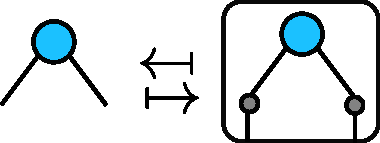
\includegraphics[scale=.4]{pictures/sigma-dot-1}} 
\end{array}
$$
\item \textbf{Associativity.}
$$
\begin{array}{c}
 \ranked{(\Sigma \cdot \Gamma)\cdot \Delta } \ \ \ranked{\to} \ \    \ranked{ \Sigma \cdot (\Gamma \cdot \Delta)}\\[5pt]
        {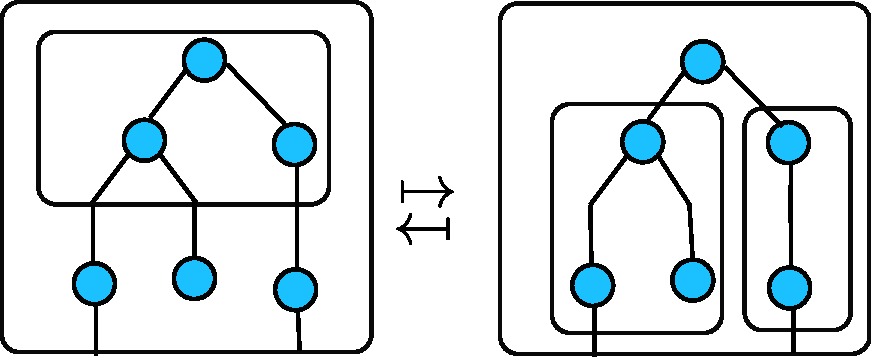
\includegraphics[scale=.4]{pictures/associativity-shallow}} 
\end{array}
$$
\item \textbf{Terms as shallow terms.}
$$
\begin{array}{c}
 \ranked {1 + \shallowterm \Sigma {\tmonad \Sigma}\ \ \to \ \  \tmonad \Sigma}\\[5pt]
        {
        \begin{tabular}{l}
            Every term is either just a port,\\ or has a root and child subterms.    
        \end{tabular}    
        }
\end{array}
$$
\item \textbf{Tensors as shallow terms.}
$$
\begin{array}{c}
\ranked {\Sigma^n \ \ \leftrightarrow \ \ \shallowterm n \Sigma}\\[5pt]
        {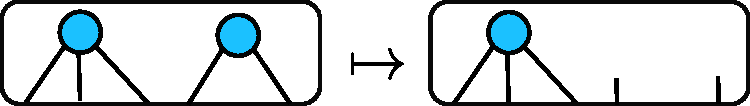
\includegraphics[scale=.4]{pictures/tensor-projection-1}}
\end{array}
$$
\end{itemize}
\end{minipage}
}
\caption{Prime functions for shallow terms.}\label{fig:prime-for-shallow-terms}
\end{figure}

\begin{figure}
\fbox{
\begin{minipage}{1\linewidth}
\begin{itemize}
\item \textbf{Unit.}
$$
\begin{array}{c}
 \ranked{\Sigma \ \ \to \ \ \reduce k \Sigma^k}\\[5pt]
        {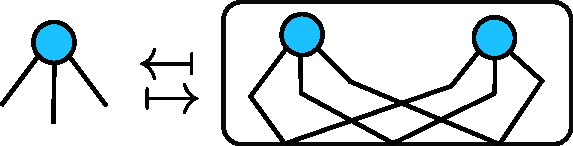
\includegraphics[scale=.4]{pictures/tensor-injection}}
\end{array}
$$
\item \textbf{Increase fold.}
$$
\begin{array}{c}
 \ranked{\reduce k \Sigma \ \ \to \ \ \reduce {k+1}\Sigma}\\[5pt]
        {
\includegraphics[scale=.4]{pictures/add-fold}}	
\end{array}$$
\item \textbf{Decrease fold.}
$$
\begin{array}{c}
 \ranked{\reduce {k+1} \Sigma \ \ \to \ \ \reduce {k}\Sigma+\bot}\\[5pt]
        {
\includegraphics[scale=.4]{pictures/reduce-fold}}	 
\end{array}$$
\item \textbf{projection of copairs.}
$$
\begin{array}{c}
   \ranked{\Sigma\product \Sigma \ \ \to \ \ \reduce 1 \Sigma}\\[5pt]
        {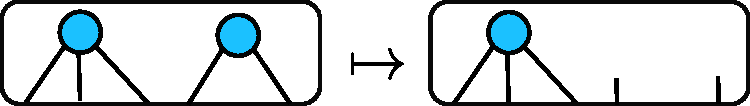
\includegraphics[scale=.4]{pictures/tensor-projection-1}}	
\end{array}$$
\end{itemize}
\end{minipage}
}
\caption{Additional prime functions for folds.}\label{fig:additional-prime-for-fold}
\end{figure}

\begin{figure}
\fbox{
\begin{minipage}{1\linewidth}
\begin{itemize}
\item \textbf{Folds over pairs.}
$$
\begin{array}{rll}
  \ranked{\reduce k (\Sigma_1 + \Sigma_2)}& \ranked{\to} & \ranked{\reduce k \Sigma_1 + \reduce k \Sigma_2}\\
         (a,i)/f & \mapsto & ((a/f),i)
\end{array}
$$
\item \textbf{Shallow terms over pairs.}
$$
\begin{array}{rll}
  {\shallowterm {(\Sigma_1 + \Sigma_2)} \Gamma} & \ranked{\to} & \ranked{(\shallowterm {\Sigma_1} \Gamma) + (\shallowterm {\Sigma_2} \Gamma)}\\
        (a,i)\tensorpair{t_1,\dots,t_n} &\mapsto& (a\tensorpair{t_1,\dots,t_n},i)
\end{array}
$$
\item \textbf{Shallow terms over copairs.}
$$
\begin{array}{c}
  \ranked{{\shallowterm {(\Sigma_1 \product \Sigma_2)} \Gamma}
   \ \  \to \ \ {(\shallowterm {\Sigma_1} \Gamma) \product (\shallowterm {\Sigma_2} \Gamma)}}\\[5pt]
        {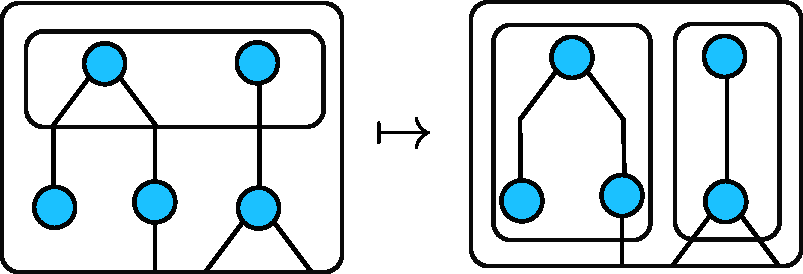
\includegraphics[scale=.4]{pictures/tensor-shallow-distrib}}
        \end{array}
$$
\item \textbf{Folds over copairs.}
$$
\begin{array}{c}
\ranked{(\reduce k \Sigma_1) \product (\reduce k {\Sigma_2}) \ \ \to \ \reduce k (\Sigma_1 \product \Sigma_2)}\\[5pt]
        {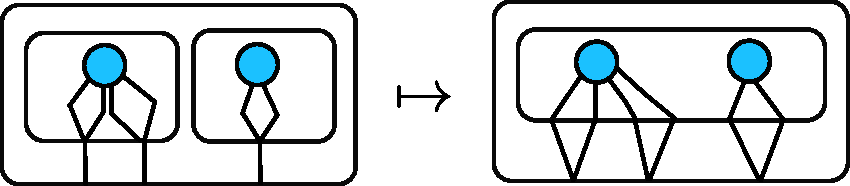
\includegraphics[scale=.4]{pictures/tensor-fold-distrib-2}}  
\end{array}
$$
\item \textbf{Folds over copairs (bis).}
$$
\begin{array}{c}
    \ranked{\reduce k (\Sigma_1 \product \Sigma_2) \ \ \to \ \ \reduce k ((\reduce k {\Sigma_1})\product (\reduce k \Sigma_2))}\\[5pt]
        {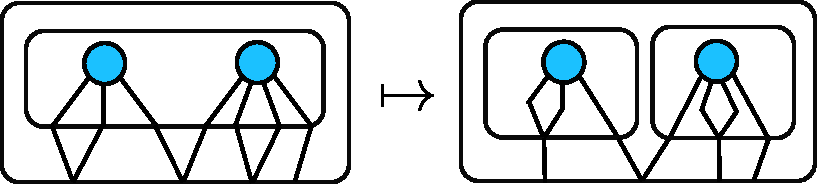
\includegraphics[scale=.4]{pictures/tensor-fold-distrib-1}}   
\end{array}
$$
\item \textbf{Shallow terms over folds.}
$$
\begin{array}{c}
 \ranked{\shallowterm \Sigma {\reduce k \Gamma}\ \ \to \ \ \reduce k (\shallowterm \Sigma {\Gamma})}\\[5pt]
 {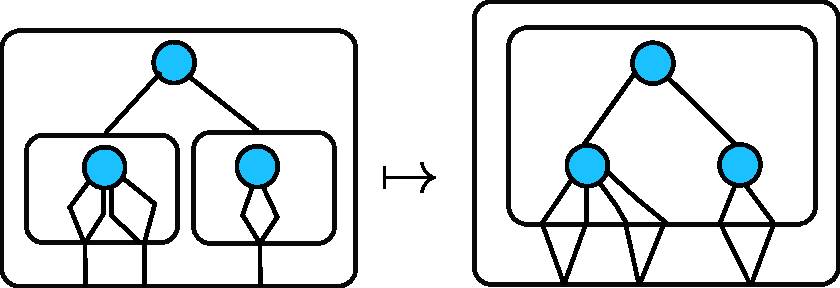
\includegraphics[scale=.4]{pictures/shallow-fold-distrib}} 
\end{array}
$$
\item \textbf{Folds over shallow terms.} 
$$
\begin{array}{c}
 \ranked{\reduce k \Sigma\cdot \Gamma\ \ \to \ \ (\reduce k \Sigma) \cdot \mati k \Gamma}\\[5pt]
 {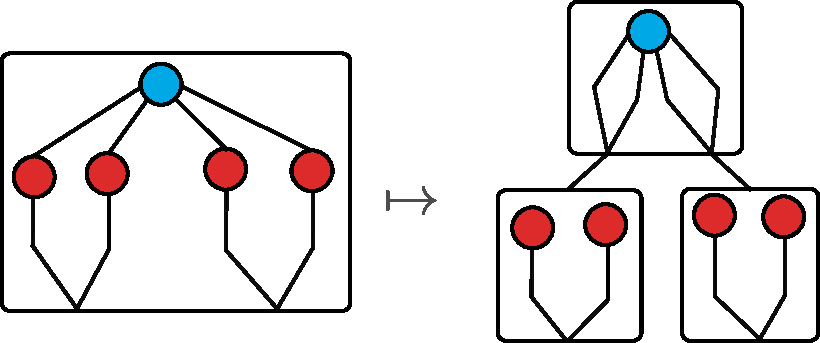
\includegraphics[scale=.4]{pictures/last-prime-function}} 
\end{array}
$$
$\rGamma$ is a set of unary elements.
\end{itemize}
\end{minipage}
}
\caption{Additional distributivity prime functions.} \label{fig:additional-distrib-prime}
\end{figure}

\begin{figure}
\fbox{
\begin{minipage}{1\linewidth}
\begin{itemize}
\item \textbf{Untwist.}
$$
\begin{array}{c}
\ranked{\tmonad {\reduce 1\Sigma} \ \  \to \ \ \reduce 1 \tmonad \Sigma}\\[5pt]
         {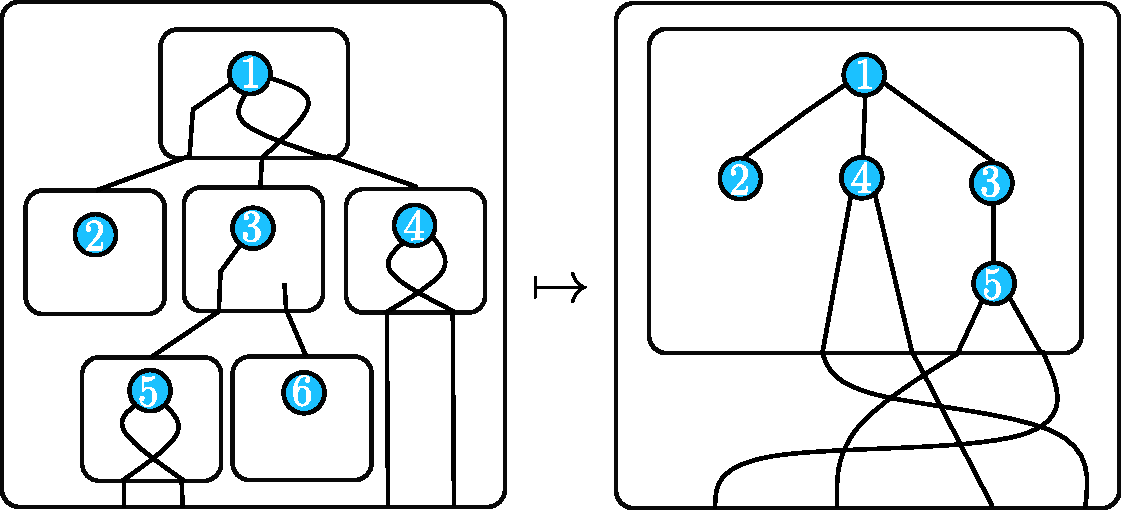
\includegraphics[scale=.4]{pictures/unfold-1}}
\end{array}
$$
\item \textbf{External fold.}
$$
\begin{array}{c}
\ranked{\tmonad {\reduce k\Sigma} \ \  \to \ \ \reduce k \tmonad \reduce k\Sigma}\\[5pt]
         {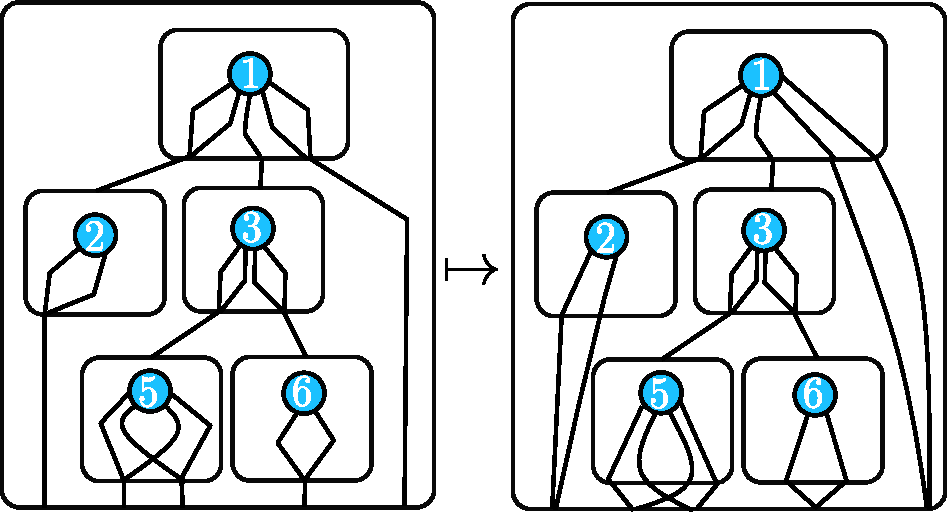
\includegraphics[scale=.43]{pictures/external-unfold-1}}
\end{array}
$$
\item \textbf{Matching.}
$$
\begin{array}{c}
\ranked{\shallowterm {\reduce k \Sigma}{\Gamma^k} \ \ \to \ \ \reduce 1(\shallowterm \Sigma \Gamma)}\\[5pt]
\includegraphics[scale=.3]{pictures/shallow-unfold}
\end{array}
$$
\end{itemize}
\end{minipage}
}
\caption{Weak forms of unfolding.}\label{fig:weak-unfolding}
\end{figure}

\subsection{The atomic functions not explained in Figure~\ref{fig:fo-term}}
\label{sec:atomic-and-combinators}
In this section, we define the atomic functions whose definitions were not given in Figure~\ref{fig:fo-term}. 




\subsubsection{Factorisations}
    Let $t \in \tmonad \rSigma$ be a term. 
    There are two equivalent definitions of factorisations of $t$. One definition is that a factorisation is an equivalence relation on non-port nodes where every equivalence class is a factor; the other definition is that it is any term $s  \in \tmonad \tmonad \rSigma$ which flattens to $t$. 
    The two definitions are easily seen to be equivalent, in the sense that there is a one-to-one correspondence between factorisation equivalences and factorisation terms.
    %  which is explained in the following picture:
    % \mypic{14}
    Suppose that $\ranked{\Sigma_1}$ and $\ranked{\Sigma_2}$ are ranked sets. The ancestor and descendant factorisations 
        \begin{align*}
            \overbrace{\ancfact}^{\text{ancestor}}, \overbrace{\decfact}^{\text{descendant}}  : \ranked{\tmonad(\Sigma_1+\Sigma_2) \to \tmonad(\tmonad \Sigma_1 + \tmonad \Sigma_2)}
        \end{align*}
        are defined as follows. Consider an input term
        \begin{align*}
            t \in \ranked{\tmonad(\Sigma_1+\Sigma_2)}.
        \end{align*}
        We say that two non-port nodes have \emph{same type} if both have labels in the same  $\ranked{\Sigma_i}$; otherwise we say that non-port nodes have \emph{opposing type}.  Call two non-port nodes \emph{ancestor equivalent}  if they have the same proper ancestors of opposing type. Call two non-port nodes \emph{descendant equivalent}  if they  are ancestor equivalent and they have the same proper descendants of opposing type. Here is a picture, with $\ranked{\Sigma_1}$ being red and $\ranked{\Sigma_2}$ being blue: 
        \begin{center}
      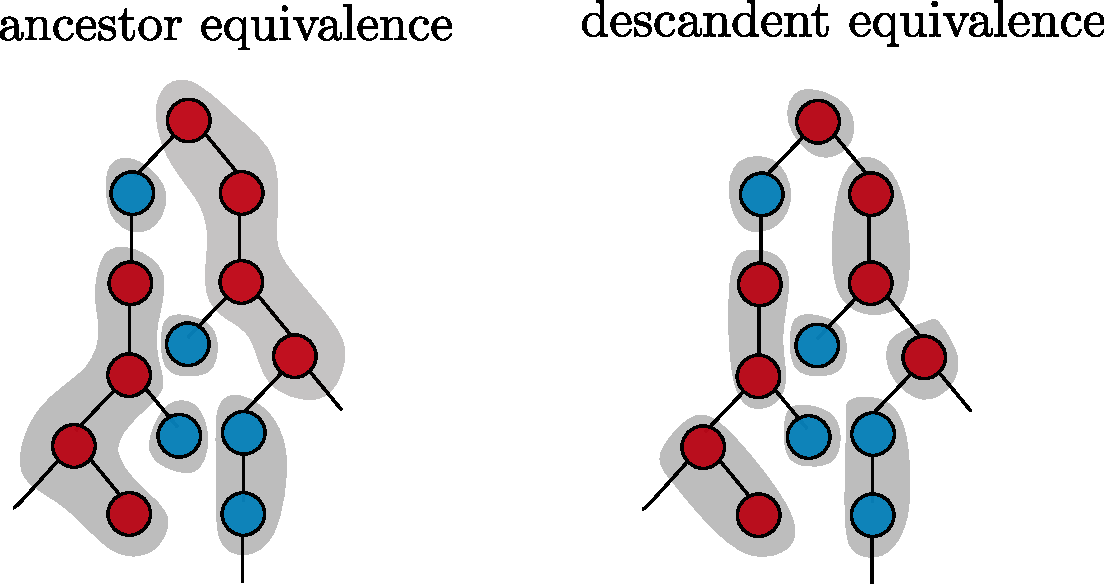
\includegraphics[scale=.4]{facto-up-down.pdf}
        \end{center}
        Both ancestor and descendant equivalences are factorisations; and in each case equivalence classes contain only nodes of same type.  The function $\ancfact$ maps a term to (the term of terms corresponding to) its ancestor equivalence relation, likewise we define $\decfact$ for  descendant factorisations.
    
        \subsubsection{Pre-order traversal.} The preorder traversal function  
        \begin{align*}
            \ranked{\preorder : \tmonad \Sigma \to \reduce 1 \tmonad (\rSigma + 0 + 2)}
        \end{align*}
        is the natural extension -- from trees to terms -- of the depth-first traversal, as explained below (the nullary grey nodes represent the labels from $\ranked 0$, and the binary grey nodes represent the labels from $\ranked 2$):
        \begin{center}
        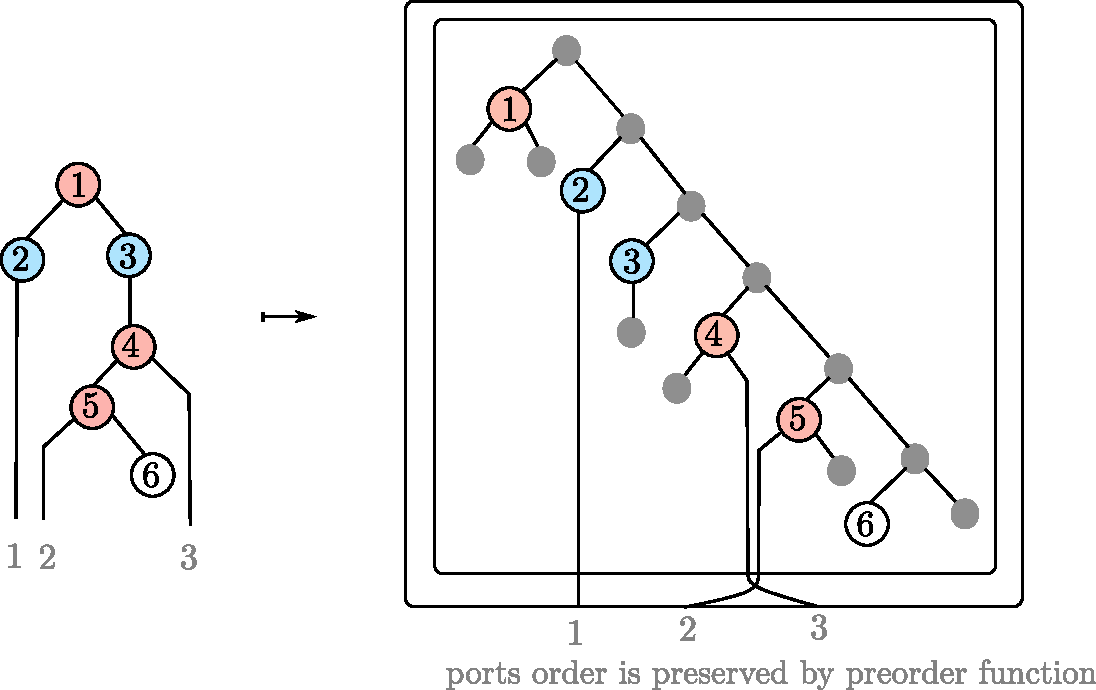
\includegraphics[scale=.45]{preorder.pdf}
        \end{center}
The $\preorder$ function respects the input port order, this is the reason  why we have a fold $\reduce 1$ in the output type. 
\subsubsection{Unfolding}
The general idea behind the  unfolding operation 
\begin{align*}
\ranked{
    \unfoldsmall : \shallowterm {(\reduce k   \Sigma)} {\Gamma^k} \to \reduce 1 (\shallowterm \Sigma \Gamma)
}
\end{align*} 
is to eliminate a $k$-fold by matching it with a $k$-th power. 
The unfolding operation is explained in the following picture for $k=2$: 
        \begin{center}
        \includegraphics[scale=.4]{shallow-unfold.pdf}
        \end{center}
% One of the main results in this paper will be  that an iterated version of the unfold operation, of type
% \begin{align*}
% \ranked{    \tmonad (\reduce k \Sigma^k) \to \reduce k (\tmonad \Sigma)^k,}
% \end{align*}
% can be derived from the other operations. 

% The formal definition is 
% \begin{align*}
% (a/f) \tensorpair{\tensorpair{b_{1,1},\ldots,b_{1,k}},\ldots,\tensorpair{b_{n,1},\ldots,b_{n,k}}} \qquad \mapsto \qquad 
% (a\tensorpair{b_{f(1)},\ldots,b_{f(\arity a)}})/g
% \end{align*}
% where $g$ is defined so that it matches ...

\noindent\begin{example}[Filter]\label{ex:filter} 
 To get a feeling for the atomic functions and combinators, we derive the function
$$ \ranked{f:\tmonad (\rSigma+\rGamma)\to\tmonad \rSigma}$$
discussed earlier, which erases the elements of $\rGamma$ from the input term, where $\rGamma$ is a finite set of unary symbols. 

Consider the atomic function $\ranked{\unit_\rSigma:\rSigma\to\tmonad\rSigma}$ and the constant function $\ranked{\mathrm{empty}:\rGamma\to\tmonad\rSigma}$ which associates to every element of $\rGamma$ the empty term. The function $\ranked{\mathrm{empty}}$ is atomic because its domain is finite. We start by lifting $\ranked{\unit_\rSigma}$ and $\ranked{\mathrm{empty}}$ to the type constructor $+$, then we compose the result with the atomic projection function as follows
\begin{align*}
\xymatrix{
    \ranked{\rSigma+\rGamma}\quad \ar[r]^-{\ranked{\unit_\Sigma+\mathsf{empty}}} & \quad \ranked{\tmonad\rSigma+\tmonad\rSigma}\ar[r]^-{} &\tmonad\rSigma
},
\end{align*}
We lift the obtained function to terms, and compose the result with the $\flatt_\rSigma$ function to obtain our function $\ranked{f}$.  
\end{example}

More examples of derived functions are given in Appendix.~\ref{sec:AppendixExamples}.
\section{Proof strategy}
\label{sec:strategy}
In this section, we present an overview of the proof of Theorem~\ref{thm:main}. The proof has five steps, which are spread across Sections~\ref{sec:to-transductions}--\ref{sec:matrix-power}, and summarised below.

\newcommand{\announce}[2]{
\begin{center}
    {\bf #1.} #2
\end{center}
}
\begin{enumerate}
\item \emph{Section~\ref{sec:to-transductions}: from the atomic functions and combinators to first-order transductions.} The easier part of Theorem~\ref{thm:main} is the  right-to-left implication, which is proved by a straightforward induction on the derivation:
\announce
{Proposition~\ref{prop:to-logic}}
{Every derivable tree-to-tree function is a first-order tree-to-tree transduction.}
 
 The remaining four steps in the proof, namely Sections~\ref{sec:fo-translation}--\ref{sec:matrix-power}, are devoted to the left-to-right implication, i.e.~showing how every first-order tree-to-tree transduction  is  derivable.

    \item \emph{Section~\ref{sec:fo-translation}: first-order rational tree functions.} We begin the proof of the left-to-right  implication  with a special case of first-order tree-to-tree transductions, which we call \emph{first-order rational tree functions.} In a first-order rational tree functions, each node is replaced by a term, with the choice of term depending on first-order definable properties of the node. Examples of first-order rational tree function include  ``remove every node with a unary label'', or ``if a leaf $x$ has at least one ancestor with label $a$, then replace the label of $x$ with the letter $c$''. First-order rational tree functions do not cover all first-order transductions, for example the pre-order function is not a rational tree function, but they are an important subcase.
    The main result of Section~\ref{sec:fo-translation} is:
    \announce
    {Proposition~\ref{prop:forat}}
    {Every first-order rational tree function is derivable.}
    The main tool used in the proof of Proposition~\ref{prop:forat} is a theorem of Schlingloff~\cite[Theorem 2.6]{schlingloff1992expressive}, which can be seen as tree version of the Kamp theorem about {\sc ltl} being  expressively complete for first-order logic.  
    \item \emph{Section~\ref{sec:stt}: streaming tree transducers. }Instead of dealing with first-order transductions, we use an automaton model that is equivalent to them. In Section~\ref{sec:stt}, we present  this  automaton model, which we call \emph{first-order streaming tree transducers}. This  is a bottom-up tree automaton, which uses registers to store parts of the output tree. The model is based on~\cite{alur2017streaming}, but it is  appropriately restricted so that it matches first-order logic, as opposed to monadic second-order logic which was used in~\cite{alur2017streaming}. The main result of Section~\ref{sec:stt} is:
    \announce
    {Proposition~\ref{prop:stt}}
    {Every first-order  tree transduction can be computed by a first-order streaming tree transducer.}
    The converse implication is also true, and follows from Propositions~\ref{prop:to-logic} and~\ref{prop:many-register}.
    
     \item \emph{Section~\ref{sec:one-register}: streaming tree transducers with one register.} By Proposition~\ref{sec:stt}, in order to prove the left-to-right implication in Theorem~\ref{thm:main}, it is enough to show that first-order streaming tree transducers can be derived using combinators from the atomic functions. As a first step, we prove the special case of one register only:
     \announce
    {Proposition~\ref{prop:one-register}}
    {For every first-order streaming tree transducer with one register, the function it computes can be derived using the combinators from the atomic functions.}
    The proof of the above result uses two main ingredients: (a) the control structure of a streaming string transducer can be simulated using first-order rational tree functions, which are covered by Proposition~\ref{prop:forat}; and (b) when there is one register only, the register updates correspond to a restricted form of $\beta$-reduction in $\lambda$-terms, which can be simulated using the atomic functions and combinators.  
    \item \emph{Section~\ref{sec:matrix-power}: reduction to one register.}  In Section~\ref{sec:matrix-power}, we complete the proof of Theorem~\ref{thm:main}, by showing that every first-order streaming tree transducer can be obtained by using the combinators and atomic functions:
    \announce
    {Proposition~\ref{prop:many-register}}
    {For every first-order streaming tree transducer, the function it computes can be derived using the combinators from the atomic functions.}
    The above result, together with Proposition~\ref{prop:stt}, completes the proof of the left-to-right implication in Theorem~\ref{thm:main}. The proof of Proposition~\ref{prop:many-register} uses a reduction to the single register case that was treated in Proposition~\ref{prop:one-register}. In the reduction, we use a type constructor called the \emph{matrix power}, which has origins in universal algebra. In Section~\ref{sec:matrix-power}, we show that (a) a transducer with many registers can be simulated by using matrix power and transducers with a single register; and (b) the matrix power and its associated operations can be simulated using our atomic operations and combinators. The proof of (b) uses a the Factorisation Forest Theorem of Imre Simon~\cite{simon_factorization_1990}.
\end{enumerate}

\newcommand{\Root}[1]{\mathsf{root}_{#1}}
\newcommand{\Port}[1]{\mathsf{port}_{#1}}
\newcommand{\Interface}[1]{\mathsf{Interface}_{#1}}
\section{Atomic functions and combinators to first-order transductions}
\label{sec:to-transductions}
In this section, we prove the right-to-left implication in Theorem~\ref{thm:main}, namely that if $\rSigma,\rGamma$ are finite ranked sets, then for every derivable function $\ranked {f : \tmonad \rSigma \to \tmonad \rGamma}$, its restriction to trees $f : \trees \rSigma \to \trees \rGamma$
is a first-order tree-to-tree transduction. The proof is a simple induction on the derivation of  $\ranked f$. In the induction, we must deal with functions that manipulate types that are more complex than trees, e.g.~tensor pairs of terms of coproducts.  To operate on such types with first-order transductions, we need to show how such types can be modelled as relational structures.


% We do this by assigning to each element $a$ in a type $\rSigma$ an associated model $\underline a$. 
% \newcommand{\structa}{\mathfrak A}
% When defining the models below, we use two types of disjoint union. 
% \begin{itemize}
%     \item For two relational structures $\structa_1,\structa_2$ over relational vocabularies $\ranked{\tau_1},\ranked{\tau_2}$, define $\structa_1 + \structa_2$ to be the  relational structure over vocabulary $\ranked{\tau_1 + \tau_2}$ defined by taking the disjoint union of the structures, and interpreting the relations of $\structa_i$ using the copy $\ranked{\tau_i}$ of the vocabulary.
%     \item For a family of $\set{\structa_i}_{i \in I}$ of relational structures over a common vocabulary $\ranked \tau$, define $\coprod_i \structa_i$ to be the structure over $\ranked \tau$ disjoint union of the structures, with all components using the common vocabulary.
% \end{itemize}


\begin{definition}[Associated models for terms, pairs, co-pairs and tensors.] \label{def:type-model} To each type  $\rSigma$ be a vocabulary, called the \emph{vocabulary of $\rSigma$}, and a map 
    \begin{align*}
        a \in \rSigma \qquad \mapsto \qquad \underbrace{\underline a \in \text{models over the  vocabulary of  $\rSigma$}}_{\text{associated model of $a$}}.
    \end{align*}
    Furthermore, for each $a \in \rSigma$ we  distinguish a  sequence (whose length is the arity of $a$) of distinguished elements in $\underline a$, which are called the ports $\underline a$.   The definitions are by induction on the structure of $\rSigma$, as given below.
    \begin{itemize}
        \item \emph{Finite ranked sets.} Elements of a ranked set   $\rSigma =  \set{a_1,\ldots,a_k}$ are modelled a using  vocabulary which has unary relations $A_1,\ldots,A_k$ and $P_1,\ldots,P_m$ where $m$ is the maximal arity of elements in $\rSigma$. 
        For $a \in \rSigma$ of arity $n$, the  universe of $\underline a$ is $\set{0,1,\ldots,n}$, with the ports being $1,\ldots,n$. 
            The  relation $P_i$  is interpreted as $\set i$ when $i \in \set{1,\ldots,n}$ and as the empty set otherwise. The relation $a_i$ is interpreted as $\set 0$ when $a = a_i$ and as the empty set otherwise. 
        \item \emph{Coproduct.}  Elements of the coproduct $\ranked{\Sigma_1 + \Sigma_2}$ are modelled using the disjoint union of the vocabularies of $\ranked{\Sigma_1}$ and $\ranked{\Sigma_2}$. 
            If an element of the coproduct comes from $\ranked{\Sigma_1}$, then its associated model is defined as for the type $\ranked{\Sigma_1}$, with  the remaining relations from the vocabulary of   $\ranked{\voctype \Sigma_2}$ interpreted   as empty sets. The definition is analogous for  elements from $\ranked{\Sigma_2}$. 
        \item \emph{Tensor product.}   Tensor pairs in   $\ranked{\Sigma_1 \otimes \Sigma_2}$ are modelled
        using the disjoint union of the vocabularies of $\ranked{\Sigma_1}$ and $\ranked{\Sigma_2}$. 
            For  $\tensorpair{a_1,a_2}$, the associated model is    the disjoint union $\underline{a_1} + \underline {a_2}$, with the relations of $\underline {a_1}$ using the    $\voctype{\ranked{\Sigma_1}}$  part of the vocabulary, and the relations of $\underline {a_2}$ using the the    $\voctype{\ranked{\Sigma_1}}$  part of the vocabulary. 
            If $n_1$ is the arity of $a_1$, then the first $n_1$ ports are inherited from  $\underline {a_1}$ and the remaining ports are inherited from  $\underline {a_2}$.
        \item \emph{Cartesian product.}   Cartesian pairs in  $\ranked{\Sigma_1 \otimes \Sigma_2}$ are modelled  using the disjoint union of the vocabularies of $\ranked{\Sigma_1}$ and $\ranked{\Sigma_2}$, plus an extra binary relation $R$.  
            The model associated to a Cartesian pair   $ (a_1,a_2)$,  is      the disjoint union $\underline{a_1} +  \underline {a_2}$, in the same sense as in the previous item for $\otimes$,  with the binary relation $R$ interpreted as 
                \begin{align*}
                    \set{(\text{$i$-th port of $\underline {a_1}$}, \text{$i$-th port of $\underline a_2$}): i \in \set{1,\ldots,\text{arity of $(a_1,a_2)$}}} 
                \end{align*}
                The ports are inherited from   $\underline {a_1}$.
        \item \emph{Folding.}   For $k \in \set{1,2,\ldots}$, elements of   $\reduce k \rSigma$ are modelled using the  vocabulary of $\rSigma$ plus two extra binary relations $<$ and $R$. If $a \in \rSigma$ has arity $nk$, then the model associated to $a/f$ -- which has arity $n$ --   is obtained from  $\underline{a}$ by adding a copy of the model
                \begin{align*}
                (\set{1,\ldots,n}, <),
                \end{align*}
        whose elements are used as the ports, and interpreting the binary relation $R$ as
        \begin{align*}
        \set{(\text{$i$-th port of $\underline a$},f(i)) : i \in \set{1,\ldots,nk}}
        \end{align*}
                
                
        \item \emph{Terms.}  Terms in $\tmonad \rSigma$ are modelled using vocabulary of $\rSigma$ extended with two fresh binary relations $\anceord$ and $\portord$. 
          Let $t \in \tmonad \rSigma$. Consider the disjoint union of models
            \begin{align}\label{eq:non-port}
                 \coprod_{x \in \text{non-port nodes in $t$}} \underline{a(x)},
            \end{align}
         where  $\underline a(x)$ is the model over vocabulary $\voctype \rSigma$ that  is defined by induction assumption.   In the above  disjoint union, the same vocabulary, namely the vocabulary of $\rSigma$,  is used  for all parts of the disjoint union. Next, consider  the model
            \begin{align}\label{eq:ports}
            (\set{1,\ldots,n}, \portord)
            \end{align}
            where $\portord$ is the natural ordering on $\set{1,\ldots,n}$. 
            The model of $t$ is defined by taking the disjoint union of the models in~\eqref{eq:non-port} and~\eqref{eq:ports}, and defining the binary relation $\anceord$ as follows.
            \begin{center}
                (fill in the definition of $\anceord$)
            \end{center}
            % It  consists of all pairs $(u,v)$ such that $u$ is the $i$-th port of $\underline{a(x)}$  some non-port node $x$, and $v$ belongs to $\underline{a(y)}$ for some node (possibly a port) $y$ which is a descendant (not necessarily proper) of the $i$-th child of $x$. The binary relation $\portletter$ is the total order 
            The ports are taken from the structure~\eqref{eq:ports}.
    \end{itemize}
\end{definition}

The above  definition creates a certain ambiguity for trees, because if $t$ is a tree over a finite ranked set $\rSigma$, then $\underline t$ can be understood in two ways: as per  Definition~\ref{def:tree-model} for trees, or as per Definition~\ref{def:type-model} when $t$ is viewed as a special case of a term $t \in \tmonad \rSigma$. Since we only use first-order transductions to transform relational structures,  this ambiguity is not a problem, because one can easily define first-order transductions which map one definition of $\underline t$ to the other.

The following lemma immediately yields the right-to-left implication in Theorem~\ref{thm:main}. It proof, which is a straightforward case analysis of all atomic functions and combinators, is in the appendix. 




  
\begin{proposition}\label{prop:to-logic} If $f : \rSigma \to \rGamma$ is derivable, then there is a first-order transduction $g$ 
    which makes the following diagram commute
    \begin{align*}
        \xymatrix@C=3cm{
            \rSigma \ar[d]_{a \mapsto \underline a}\ar[r]^f &  \rGamma \ar[d]^{a \mapsto \underline a} \\
            \text{models over the vocabulary of  $ \rSigma$} \ar[r]_g &  \text{models over the vocabulary of  $ \rGamma$}.
        } 
    \end{align*}
    
\end{proposition}




\section{First-order  relabellings}\label{sec:fo-translation}
In this section we prove derivability of the first computation step used in first-order register transducers.
\begin{proposition} \label{prop:forat}    
    Every first-order relabelling is derivable.
\end{proposition}
To prove the proposition, we use a decomposition of first-order relabellings into simpler functions, in the style of the Krohn-Rhodes theorem. 
%  a characterisation of first-order logic on trees in terms of temporal logic, which was proved by Schlingloff~\cite[Theorem 4.5]{schlingloff1992expressive}. The operators in this temporal logic (which are tree variants of the since and until operators of {\sc ltl}) can be viewed as very simple first-order relabellings; by the completeness result of Schlingloff it is enough to show that these operators are derivable.  
We use the name \emph{unary query} for a first-order formula with one free variable over the vocabulary of trees. This assumes some implicit alphabet $\rSigma$.
For a  unary query,  define its  \emph{characteristic function},  of type
\begin{align*}
 \trees \rSigma \to \trees (\ranked{\rSigma + \rSigma}),
\end{align*}
to be the function which replaces the label of each node by its first or second copy, depending on whether the node is selected by the query. This is a special case of a first-order relabelling. The key to Proposition~\ref{prop:forat} is the following  lemma, which decomposes first-order relabellings  into characteristic functions of certain basic unary queries.

\begin{lemma}\label{lem:schlingloff} Every first-order relabelling can be obtained by composing the following functions:
    \begin{enumerate}
        \item \label{it:relabelling} \emph{Letter-to-letter homomorphisms}. For  every finite $\rGamma,\rSigma$ and $\ranked {f : \rSigma \to \rGamma}$, its tree lifting $\trees \ranked f : \trees \rSigma \to \trees \rGamma$.
        \item \label{it:temporal-operators} For every finite  $\rSigma$ and its subsets $\rDelta, \rGamma \subseteq \rSigma$, the characteristic functions of the following unary queries over alphabet $\rSigma$:
        \begin{enumerate}
            \item \label{it:child} \emph{Child:} $x$ is an $i$-th child, for $i \in \set{1,2,\ldots}$
            \begin{align*}
            \child i (x); 
            \end{align*}
             \item \label{it:until} \emph{Until:}  $x$ has a descendant $y$ with label in $\rDelta$, such that all nodes strictly between $x$ and $y$ have label in $\rGamma$
             \begin{align*} 
                  \exists y\ y > x \land \rDelta(y) \land  \forall z \ (x < z < y \Rightarrow \rGamma(z));
             \end{align*} 
             \item \label{it:since}\emph{Since:} $x$ has an ancestor $y$ with label in $\rDelta$, such that all nodes strictly between $x$ and $y$ have label in $\rGamma$
             \begin{align*}
                  \exists y\ y < x \land \rDelta(y) \land  \forall z \ (y < z < x \Rightarrow \rGamma(z)).
             \end{align*} 
        \end{enumerate}
    \end{enumerate}
    
\end{lemma}

The  lemma uses a theorem of   Schlingloff~\cite[Theorem 2.6]{schlingloff1992expressive}, which says  that all first-order definable tree properties can be defined using a temporal logic with operators similar to the ones used in items~\ref{it:temporal-operators} of the lemma. Note that the temporal logic is a two-way logic, because  \emph{until} depends on the descendants of the node $x$, while \emph{since} depends on the ancestors. In fact, there is no temporal logic which characterises first-order logic, uses only descendants, and has finitely many operators~\cite[Theorem 5.5]{bojanczykWreathProductsForest2012}. 
The exact reduction to Schlingloff's theorem is  in Appendix~\ref{sec:AppendixForat}.

It remains to show that all of the functions from Lemma~\ref{lem:schlingloff} are derivable. 
The letter-to-letter homomorphisms from item~\ref{it:relabelling} are   a special case of homomorphisms discussed in Example~\ref{ex:filter}, and hence derivable. In Appendix~\ref{sec:AppendixForat}, we show that the functions from item~\ref{it:temporal-operators} are also derivable. In the proof, a key role is played by the factorisation functions discussed in Section~\ref{sec:factorisation-functions}. 
% i lemmas~\ref{lem:nextmod}, \ref {lem:untilmod} and \ref{lem:sincemod}. 
\section{The proof strategy}

\subsection{Streaming tree transducers}
% We use an algebraic syntax for streaming tree transducers. 
% \emph{Linear polynomials.} Suppose that $\Sigma$ is a finite ranked alphabet.  For a ranked set $X$, define a \emph{polynomial with variables $X$ over $\Sigma$} to be any term in $\trees (\Sigma + X)$. Given such a polynomial $p$, and an arity preserving valuation $v : X \to \trees \Sigma$, we define $p(v)\in \trees \Sigma$ to be the term obtained from $p$ by replacing each variable with its value under $v$. The arity of $p(v)$ is the same as the arity of $p$.  A polynomial is called \emph{linear}, or non-duplicating, if each variable from $X$ is used at most once.

% \begin{definition}
%     For a ranked set $\Sigma$, define $\aalg_\Sigma$ to be the following multisorted algebra. 
%     \begin{itemize}
%         \item The sorts are arities, i.e.~numbers in $\set{0,1,2,\ldots}$, and elements of sort $n$ are $n$-ary terms in $\trees  \Sigma$;
%         \item The operations are the polynomial operations. 
%     \end{itemize}
% \end{definition}




\paragraph*{Register valuations and updates.}   Let $\Sigma, R$ be finite ranked sets, which are called the \emph{output alphabet} and \emph{register names} respectively.  
A \emph{register valuation} (over $\Sigma$ and $R$) is defined to be any arity-preserving function
\begin{align*}
    v : R \to \trees \Sigma
\end{align*}
For  $k \in \set{0,1,\ldots}$, a \emph{$k$-ary register update} (over $\Sigma$ and $R$) is defined to be any an arity-preserving function
\begin{align*}
    u : R \to \trees ( \Sigma + \underbrace{R + \cdots +R}_{\text{$k$ times}})
\end{align*}
A $k$-ary register update can be applied to a $k$-tuple of register valuations, yielding a new register valuation, as illustrated in the following picture:
\begin{center}
    picture here
\end{center}
A register update is called \emph{copyless} if each copy of a register name is used at most once. More formally,for each $i \in \set{1,\ldots,k}$ and each register name $r \in R$, there is at most one $s \in R$ such that the $i$-th copy of $r$ appears in $u(s)$, and furthermore this copy appears at most once in $u(s)$. 


\begin{definition}[Streaming Tree Transducer]
    A \emph{streaming tree transducer} consists of 
\begin{itemize}
    \item Input and output alphabets $\Sigma$ and $\Gamma$, which are finite ranked sets;
    \item A finite set of states $Q$, not ranked.
    \item A finite set of regsiters $R$, ranked.
    \item For each input letter $a \in \Sigma$, of arity $n$, a transition function
 \begin{align*}
     Q^n \to Q \times \text{($n$-ary register updates over $\Gamma$ and $R$)}
 \end{align*}
 \item An ouptut function
 \begin{align*}
     Q \to \treesz(\Gamma + R)
 \end{align*}
\end{itemize}
\end{definition}

For a streaming tree transducer and a tree over the input alphabet, one defines a pair (state, register valuation)
by induction on the size of the tree, using the transition function, in the natural way. Suppose that $t$  is a tree over the input alphabet, and let $(q,v)$ be the associated states and register  valuations. To obtain the output for the tree $t$, one applies the output function to $q$, yielding a tree over $\Gamma + R$, and then substitutes the register names according to the register valuation $v$. 


\begin{definition}[First-order Definable Streaming Tree Transducer]\ 
    A streaming tree-to-tree transducer is called \emph{first-order definable} if for every state $q$, the set of trees which get evaluated to state $q$ is a first-order definable tree language.
\end{definition}    
\begin{theorem}\label{thm:sst}
    The following classes of tree-to-tree transductions are the same:
    \begin{itemize}
        \item  \mso tree-to-tree transductions;
        \item streaming tree transducers.
    \end{itemize}
    First-order  tree-to-tree transductions are equal to first-order definable streaming tree transducers.
\end{theorem}

The result for \mso, adjusting for a different syntax,  was proved in~\cite[Theorem 4.6]{alur2017streaming}. The result for fo uses the same ideas. A proof is in the appendix.
\begin{center}
    do this appendix 
\end{center}

\subsection{A decomposition}


\begin{definition}[Fo translation]
    An fo-translation is a tree-to-tree transduction
    \begin{align*}
      f :   \treesz \Sigma \to \treesz \Gamma
    \end{align*}
    which is given by a family of unary queries 
    \begin{align*}
        \set{\varphi_a(x)}_{a \in \Gamma}
    \end{align*}
    over input alphabet $\Sigma$ such that for every tree $t \in \treesz \Sigma$ and node $x$ in $t$, there is exactly one $a \in \Gamma$ such that $\varphi_a(x)$ is true, and furthermore the arity of $a$ is the same as the arity (number of children) of $x$.  The output tree $f(t)$ is defined by replacing the label of each node $x$ by the unique $a$ which makes $\varphi_a(x)$ true.
\end{definition}
% \begin{lemma}
%     Every first-order streaming tree transducer is equivalent to one where all registers have arity 1.
% \end{lemma}



\begin{lemma}\label{lem:decomposition-of-fo-transductions} Every first-order tree function $f$  can be decomposed as
    \begin{align*}
        \xymatrix@C=2cm{\treesz \Sigma \ar[d]_f \ar[r]^g& \treesz \overbrace{(\Delta \otimes \cdots \otimes \Delta)}^{\text{$k$ times}} \ar[d]^{\mathsf{unfold}} \\   \treesz \Gamma  & \treesz \Delta \ar[l]^h}
    \end{align*}
    where 
    \begin{itemize}
        \item $\Delta$ is a finite ranked alphabet and $k \in \set{1,2,\ldots}$;
        \item $g$ is an fo-translation;
        \item $h$ is recognised by a first-order streaming transducer which has one register, and that register has arity one.
    \end{itemize}
\end{lemma}

By the above lemma, it remains to deal with first-order translations and streaming tree transducers with one unary register. This we do in Sections~\ref{sec:fo-translation} and~\ref{sec:one-register}.

\section{Evaluation of simply typed linear terms}
\label{sec:one-register}

In this section, we consider an important example of derivable term transformations, namely evaluating (i.e.~computing $\beta$-normal forms of)  simply typed  $\lambda$-terms that are linear in the sense that each bound variable is used exactly once in its scope. Apart from its independent interest, evaluation of $\lambda$-terms will  be used in the proof our main theorem. 



\newcommand{\otype}{o}
We assume that the reader is familiar with the basic notions of the simply typed $\lambda$-calculus; more detailed definitions can be found in~\cite{sorensen_lectures_2006}. Define  \emph{simple types} to be expressions  generated from an atomic type $\otype$ using a binary arrow constructor, as in the following examples:
    \begin{align*}
        \otype \qquad \otype \to \otype \qquad (\otype \to \otype) \to (\otype \to \otype) \qquad \cdots 
    \end{align*}
Let $X$ be a set of variables, each one with an associated simple type.  A $\lambda$-term over these variables can be seen as a tree over the ranked alphabet
\begin{align*}
      \overbrace{\set{x : x \in X}}^{\text{arity 0}} \cup \overbrace{\set{\lambda x : x \in X}}^{\text{arity 1}} \cup  \overbrace{\set @}^{\text{arity 2}}
\end{align*}
where @ is the application symbol that is used to apply one term to another.
We say that a $\lambda$-term is \emph{well-typed} if one can associate  to it  a simple type according to the usual typing rules of simply typed $\lambda$-calculus\footnote{
    Here we assume that the variables are typed, but the types for the remaining $\lambda$-terms need to be inferred. We could adopt a different approach, more thoroughly in the style of Church, where all term constructors (application and $\lambda$-abstraction) come decorated with the type of the resulting term. We do not do this to make  notation lighter, and also because one show -- see the appendix -- that first-order logic is enough to reconstruct the type of a term once the types of the variables are known. 
}, see~\cite[Definition 3.2.1]{sorensen_lectures_2006}. Because the variables are typed, a  $\lambda$-term can have either a unique type, or it is not well-typed.  Here is an example of a well-typed $\lambda$-term: 
\mypic{45}
We use the standard notion of $\beta$-reduction for $\lambda$-terms, see~\cite[Definition 1.2.1]{sorensen_lectures_2006}. 
Because of normalisation and confluence for the simply typed $\lambda$-calculus, every well-typed $\lambda$-term has a unique normal form, i.e~a $\lambda$-term to which it $\beta$-reduces (in zero or more steps), and which cannot be further $\beta$-reduced.


\begin{example}\label{ex:exponential}
    Because of iterated duplication, the normal form of a $\lambda$-term can be exponential. Assume that we have two variables $\typevar x  \otype$ and $\typevar y {\otype \to \otype \to \otype}$ and consider the $\lambda$-terms defined by:
    \begin{align*}
        M_0 \eqdef \typevar x \otype \qquad M_{n+1} = (\lambda \typevar x  \otype . \typevar y {\otype \to \otype \to \otype}  \typevar x  \otype \typevar x  \otype)M_n.
    \end{align*}
    The $\lambda$-term $M_n$ is well-typed and of type $\otype$. It has size linear in $n$, but its normal form has size exponential in $n$. 
    % as shown in the following picture, which uses variables $x : \otype$ and  $z : \otype \to \otype \to \otype$.
    % \mypic{44}
\end{example}
As witnessed by the above example, normal forms can be exponential size (or worse, see~\cite[Section 3.6]{sorensen_lectures_2006}), and therefore they cannot be computed  using derivable functions or first-order transductions, because the latter have linear size outputs. To avoid this problem, we  limit attention to linear $\lambda$-terms: a $\lambda$-term is called \emph{linear} if every bound variable is used exactly once in its scope. Here is an example: 
\mypic{43}
For linear $\lambda$-terms, each step of $\beta$-reduction reduces the number of nodes by exactly 3, and therefore the normal form is linear in the size of (in fact, smaller or equal to) the original term. 

Linearity alone is not enough to normalise terms with first-order transductions. Another obstacle is terms that use types of unbounded complexity, as illustrated in the following example. 

\begin{example}
Consider the following $\lambda$-terms, which have types of unbounded size:     \begin{align*}
        M_0 \eqdef \typevar u {\otype \to \otype}  \qquad M_{n+1} \eqdef \overbrace{\lambda \typevar x {\otype}. \lambda \typevar y {\otype}.   M_n (\typevar z {\otype \to \otype \to \otype}  \typevar x {\otype} \typevar y {\otype}).}^{\text{type} \overbrace{\otype \to \otype \to \cdots \to \otype}^{\text{$n+1$ arrows}}}
    \end{align*}
    Apart from having large types (although still of rank 1, as described in~\cite[Exercise 3.6.7]{sorensen_lectures_2006}), these  $\lambda$-terms are simple: they use four variables (although the bound variables are reused), and are linear, because each bound variable is used exactly once in its scope. 
    To $M_n$, apply  $m$ arguments of type $\otype$:
    \begin{align}\label{eq:complicated-term}
    M_n \overbrace{\typevar v \otype \ \typevar v {\otype} \cdots \typevar v{\otype} }^{\text{$m$ times}}.
    \end{align}
    We claim that the above $\lambda$-term cannot be normalised using a first-order transduction, or even a monadic second-order transduction. In order to normalise, a transduction would need to be able to compare the numbers $n$ and $m$ as follows:  if $m < n$  the normal form contains $\lambda$, if $m=n$  the normal form does not contain $\lambda$, and if $m > n$ then the normal form is undefined because the $\lambda$-term is not well-typed.  Whether or not a $\lambda$-term (seen as a tree over a finite alphabet) contains $\lambda$ is a first-order definable property, and first-order definable properties are preserved under inverse images of first-order transductions. Therefore, if normalisation would be a first-order transduction,
then there would be a first-order formula which would be true for terms of the form~\eqref{eq:complicated-term} with $m>n$ and which would be false for terms of the form~\eqref{eq:complicated-term} with $m=n$. Such a formula cannot exist (even if we allow monadic second-order logic), which can be shown using a pumping argument or Ehrenfeucht-Fra\"iss\'e games. 
\end{example}

The above example explains why we need to bound the size of types that occur in subterms, motivating the following definition:  we say that a $\lambda$-term uses only types from a finite set of simple types $\typeset$ if all  subterms have types in $\typeset$.  Once we assume that $\lambda$-terms are linear, use a fixed finite set of bound variables, and use only types from a fixed finite set of simple types, then normalisation can be done by a derivable function, and therefore also by a first-order tree-to-tree transduction: 

\begin{theorem}\label{thm:normalise} Let $X$ be a finite set of simply typed variables, and let $\typeset$ be a finite set of simple types.
    The following tree-to-tree function is derivable (i.e.~it is the tree restriction of a derivable function on terms):
    \begin{align*}
        M \in \text{$\lambda$-terms over variables $X$} \qquad \mapsto \qquad \begin{cases}
            \text{normal form of $M$} & \text{if $M$ is linear, well-typed,}\\
            & \text{and uses only types from $\typeset$;}\\
            M & \text{otherwise}.
        \end{cases}
    \end{align*}
\end{theorem}

% Actually, we prove a stronger result, namely that the above function is derivable. In the end, of course, we will prove that all first-order tree-to-tree transductions are derivable, but our proof of this fact will use the derivability of normalisation as stated in Theorem~\ref{thm:normalise}.



% Recall that elements of $\tmonad \rSigma$ are defined to be trees over $\rSigma + \varnames$, where 
% \begin{align*}
%     \varnames = \set{x_1,x_2,\ldots}
% \end{align*}
% is a fixed set of  variable names that are used for ports. In this section, we view $\varnames$ as a simply typed set, where all variables $x_1,x_2,\ldots$ have the same simple type $\otype$.  Under this convention, we can view
% \begin{align*}
%     \tmonad (\overbrace{\set{x : x \in X}}^{\text{arity 0}} \cup \overbrace{\set{\lambda x : x \in X}}^{\text{arity 1}} \cup  \overbrace{\set @}^{\text{arity 2}})
% \end{align*}
% as a set of $\lambda$-terms. This is exactly the set of those $\lambda$-terms over variables $X + \varnames$ where: (a) variables from $\varnames$ are never bound; and (b) there is some $n$ such that each of the variables $x_1,\ldots,x_n \in \varnames$  appears as a free variable exactly once  and the remaining variables in $\varnames$ do not appear at all. If $S$ is a finite set of simple types, then define  $\linterm S X$ to be those terms in .. which are linear and $S$-typed. 

% Computing the normal form is beyond the scope of first-order transductions, the principal reason being that first-order transductions have linear size outputs, while normalisation can incur a blowup that is exponential or larger,
%  In Section~\ref{sec:lambda}, we will show that normalisation can be computed by a first-order transduction, assuming that: (a) the input terms are linear, which means that each bound variable is used exactly once in its scope; (b) we place an upper bound on the complexity of types used in subterms. 

% as discussed in Example~\ref{ex:labmda-terms}.  We show that the tree-to-tree function which inputs a  term and outputs its normal form can be derived, assuming that bound variables are used exactly one and there is a bound on the number of distinct terms types that can appear in the term. 

% Let $X$ be a typed set, i.e.~a set of variables with associated simple types. As in  Example~\ref{ex:labmda-terms},  we view $\lambda$-terms with variables of $X$ as trees over an ranked alphabet $\lamrank X$. 

% \begin{lemma}
%     For every typed set $X$ and every finite set $S$ of simple types, the tree language 
%     \begin{align*}
%         \set{ M \in \trees \lamrank X : \text{$M$ is well-typed and all subterms have type in $S$}}
%     \end{align*}
%     is first-order definable 
% \end{lemma}



% We say that a function $\ranked f : \linterm S X \rto \linterm S Y$ is \emph{derivable} if it can be extended to a derivable function $\ranked g : \tmonad \lamrank X \rto \tmonad \lamrank X$. The main result of this section is that normalisation is derivable, for every fixed finite $X$ and $S$. 
% \begin{proposition}\label{prop:one-register} 
%     For every typed set $X$ and every finite set $S$ of simple types, the function 
%     \begin{align*}
%         M \in  \linterm S X \qquad \mapsto \qquad \text{normal form of $M$} \in  \linterm S X
%     \end{align*}
%     is derivable.
% \end{proposition}

\section{Matrix power} 
\label{sec:matrix-power}
In this section, we define the matrix power, which can be seen as a way of representing several trees in one. %Roughly speaking, the several trees are the contents of registers in a register automaton.
%, and the single tree that represents them is the computation tree of the register automaton.  We then show that several trees stored in a computation  can be unfolded in a derivable way. 

\begin{definition}
    [Matrix power] For $k \in \set{1,2,\ldots}$ define the $k$-th matrix power\footnote{
        The name  matrix power is based the matrix power in  universal algebra (for the latter, see~\cite{Taylor1975} or~\cite{szendrei1990simple}). Roughly speaking, the restrictions that we place on the original definition correspond to the single-use and monotone conditions from Definition~\ref{def:stt}. 
     } of a ranked set $\rSigma$ 
to be 
\begin{align*}
 \mati k \rSigma \quad \eqdef \quad \ranked{\reduce k \rSigma^k}.
\end{align*}
\end{definition}

Here is a picture of a binary element in the matrix power, where $k=3$:
\begin{center}
\includegraphics[scale=.4, page=85]{pics.pdf}
\end{center}

A matrix power of arity $n$ is used as an abstraction of an $n$-ary register update $\ranked{R\to \tmonad(\Gamma+R+\dots+R)}$. The number $k$ represents the number of registers (that is the size of $\ranked {R}$), and each letter from $\rSigma$ represents a register update (that is, an element of $\ranked{\tmonad(\Gamma+R+\dots+R)}$). When two letters share the same port in the matrix power, this means that the corresponding register updates call the same component of $\ranked{R+\dots+R}$ in their definition, the position in the fold indicates which precise register is called. For instance, the register update above is an abstraction of the following binary register update of registers $r, s$ and $t$:
   \begin{center}
   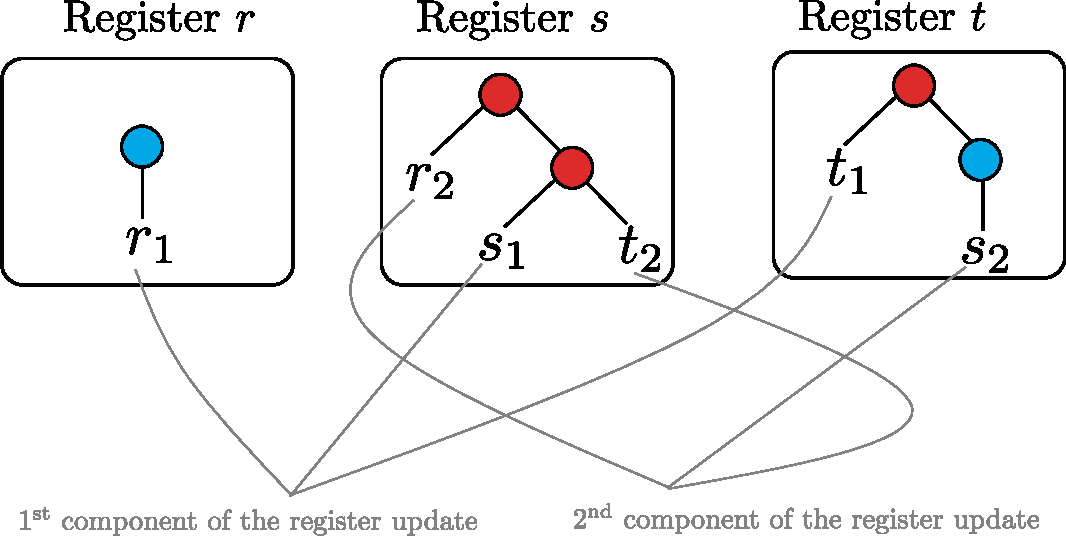
\includegraphics[scale=.3]{register-update-matrix-power.pdf}
   \end{center}
When we run a STT on an input tree, we decorate it with register updates following the transition function. In order to evaluate this tree, the first thing to do is to determine, for each register update of the root, its "dependency tree" that is to say the register updates they call, inductively. When register updates are abstracted by matrix powers, this operation of determining the dependency tree is what we call \emph{unfolding}. We illustrate it by the following example 
\begin{center}
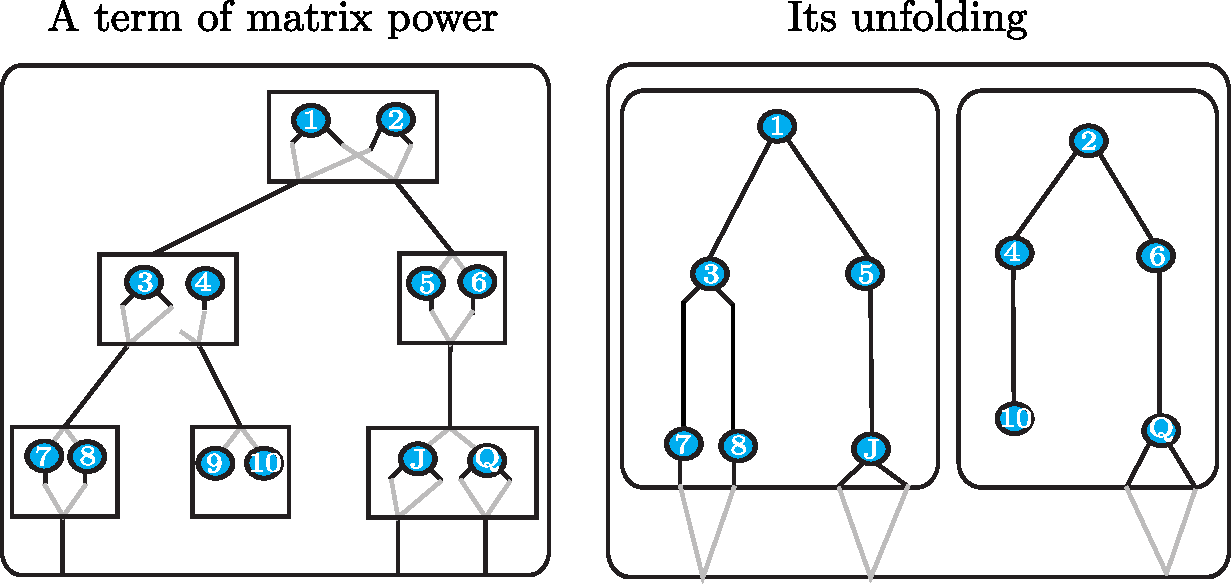
\includegraphics[scale=.38]{unfold-matrix-power}
\end{center}
Formally, \emph{unfolding} is a function of type
\begin{align*}
    \ranked{\unfold : \tmonad \mati k \rSigma \to \mati k {(\tmonad \Sigma)} }
    \end{align*}
 which is defined as follows by induction on the size of the input term. If the input is an empty term, then the output is this term:
\begin{center}
\includegraphics[scale=.3, page=83]{pics.pdf}
\end{center}
Otherwise, if the input is a nonempty term $a(t_1,\ldots,t_n)$ then the output is obtained by first applying unfolding to to the smaller terms $t_1,\ldots,t_n$, and then applying the following derivable function, which we call \emph{shallow unfold}. 
\begin{align*}
    \ranked{
        \xymatrix{
            \shallowterm{\mati k \rSigma} {\mati k \rGamma}  \ar[r] & \mati k {(\shallowterm \Sigma \Gamma)}.
        }
    }
\end{align*}
Here is a picture of unfolding for shallow terms:
\begin{center}
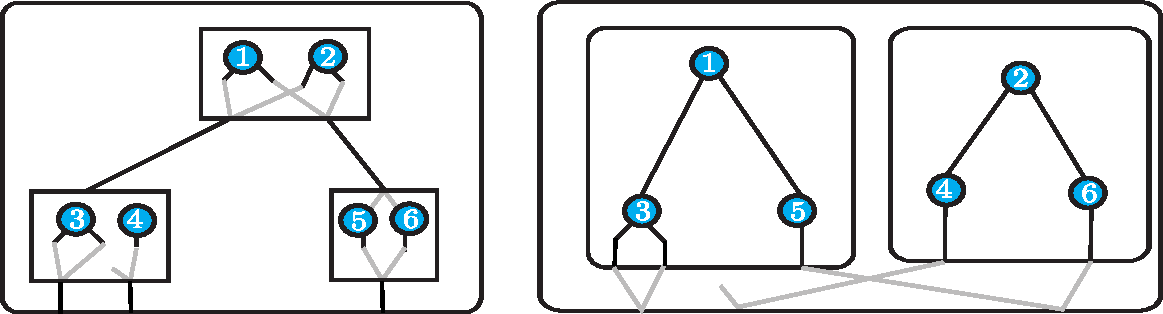
\includegraphics[scale=.4]{unfold-shallow}
\end{center}
More formally, unfolding for shallow terms is defined to be   the composition of the following functions
    \begin{align*}
        \xymatrix@R-1pc@C=3.2cm{
          {\begin{array}{c}
          \shallowterm{\mati k \rSigma} {\mati k \rGamma} \\{=\shallowterm{\reduce k {\Sigma^k}}{\reduce k {\Gamma^k}}}
          \end{array}}  \ar[d]_{{\mathrm{Commutativity}}}\ar[r]^{\mathrm{Shallow\  unfold}} &  {\begin{array}{c}
         \ranked{\mati k {(\shallowterm \Sigma \Gamma)}} \\=  \ranked{ \reduce k(\shallowterm{\Sigma}{ {\Gamma}})^k}
          \end{array}} \\
             \reduce k(\shallowterm{\reduce k {\Sigma^k}}{ {\Gamma^k}})  \ar[r]_{{\mathrm{Matching}}} &  \ranked{ \reduce k(\shallowterm{\Sigma^k}{ {\Gamma}}) } \ar[u]_{\mathrm{Commutativity}} 
        } 
    \end{align*}
Since our prime functions and combinators do not have any general mechanisms for induction, it is not clear how to derive the unfolding operation. In fact, it is not derivable in general, but it will become derivable after imposing a monotonicity requirement. The need for this condition is shown in Example~\ref{eq:twist}.  Let us define it in the following.

For a port $i$ in an element of the matrix power $a/f \in \mati k \rSigma$ define its \emph{twist} to be the partial function from $\set{1,\ldots,k}$ to itself 
which is the composition of 
\begin{align*}
\xymatrix{
    [1,k] \ar[r]^-{j \mapsto {(j,i)}} & [1,k] \times [1,n] \ar[r]^-{f^{-1}} & [1,\arity a] \ar[r] & [1,k]
}
\end{align*}
where the last function maps each port of the tuple $a$ to the coordinate of the tuple that created that port. Here is a picture:
\begin{center}
\includegraphics[scale=.3, page=87]{pics.pdf}
\end{center}
 We say that an element of the $k$-matrix power is \emph{monotone} if all of its ports have monotone twist. For instance, the right example above is not monotone.
 We are now ready to state the principal result of this section.

\begin{proposition}\label{prop:monotone-unfold}
    For every finite ranked set $\rSigma$ and every $k \in \set{1,2,\ldots}$ there is a derivable function 
    \begin{align*}
    \ranked{ f : \tmonad \mati k \Sigma \to \mati k {(\tmonad \Sigma)}}
    \end{align*}
    which coincides with term unfolding for monotone inputs.
\end{proposition}
The proof of the  above lemma is one of the main technical contributions of this paper, and it is given in the appendix. One of the ingredients of the proof is a first-order (in fact, derivable) version of the Factorisation Forest Theorem for trees, which is based in Colcombet's splits from~\cite{colcombetCombinatorialTheoremTrees2007}.  

%\begin{corollary}\label{cor:matrix-power}
%    Let $\rSigma$ be a finite set and let $\rDelta \subseteq \mati k \rSigma$ be a finite set which contains only monotone elements. Then one can derive the tree-to-tree function
%    \begin{align*}
%    f : \trees \rDelta \to \trees \rSigma  \qquad t \mapsto \text{first tree in the unfolding of $t$.}
%    \end{align*}
%\end{corollary}
% Let $\alg$ be an algebra and let $k \in \set{1,2,\ldots}$. How should the $k$-th power of the algebra be defined? For the domain, we use  $k$-tuples from the domain of $\alg$.  What about the operations? A natural   approach is to define the $n$-ary operations to be  $k$-tuples of $n$-ary operations from $\alg$, acting coordinate-wise. Because of the coordinate-wise action,  the coordinates in the product are independent of each other. This will be insufficient for our intended application, where the algebra $\alg$ is meant to represent individual register automaton, since the contents of register $r$ in the output of a register update depend on the contents of other registers in the input valuation . To  model this interdependence, we use a more sophisticated notion of power, 
% defined below.
% \begin{definition}
%     For an algebra $\alg$ and $k \in \set{1,2,\ldots}$, the $k$-th matrix power\footnote{
%         The definition of matrix power that we use is a special case of the original definition of matrix power from universal algebra (for the latter, see~\cite{Taylor1975} or~\cite{szendrei1990simple}). Roughly speaking, the restrictions that we place on the original definition correspond to the single-use and monotone conditions from Definition~\ref{def:stt}. 
%     } of $\alg$ is defined as follows. The domain and signature are defined by
%     \begin{align*}
%     \overbrace{(\algdom \alg)^k}^{\text{domain}} \qquad \overbrace{
%         \ranked{\reduce k ((\algops \alg)^k)}}^{\text{signature}}
%         \end{align*}
%         while the  shallow product operation is defined by
%         \begin{align*}
%             \ranked{
%         \xymatrix{
%             \shallowterm {\reduce k (\algops \alg)^{k}} {{(\algdom \alg)}^k} \ar[d] \\
%             \shallowterm {(\algops \alg)^{k}} {{(\algdom \alg)}} \ar[d] \\
%             (\shallowterm {(\algops \alg)} {{(\algdom \alg)}})^k
%          \ar[d]\\
%             (\algdom \alg)^k
%         }
%         }
%         \end{align*}
% \end{definition}

% By definition, if an algebra has a derivable shallow product, then the same is true for its  matrix powers, i.e.~for every $k$ the shallow product in the $k$-th matrix power is derivable. The following proposition -- which is much harder to show -- states a similar implication for  (not necessarily shallow) products.  
% \begin{proposition}\label{prop:matrix-power} If an algebra has a derivable product, then the same is true for its matrix powers.
% \end{proposition}
%



\section{Monadic second-order transductions}
\label{sec:mso-trans}
Our main theorem characterises first-order tree-to-tree transductions. We finish the paper by extending the notion of derivability so that it captures  \mso tree-to-tree transductions. 
Our solution is not particularly subtle. We simply add, as prime functions, all \mso relabellings, which are defined the  same way as the first-order relabellings from Definition~\ref{def:forat}, except that the unary queries can use \mso logic instead of first-order logic. 

\begin{theorem}\label{thm:mso-transductions}
    A tree-to-tree function is an \mso  transduction if and only if it can be using  Definition~\ref{def:derivable-function}  extended by  adding  all \mso relabellings as prime functions. 
\end{theorem}
\begin{proof}
    In~\cite[Corollary 1]{colcombetCombinatorialTheoremTrees2007}, Colcombet shows that every \mso formula on trees can be replaced by a first-order formula that runs on an \mso relabelling of the input tree. Applying that result to transductions, we see that every \mso tree-to-tree transduction can be decomposed as: (a) an \mso relabelling; followed by (b) a first-order tree-to-tree transduction.  The theorem follows.
\end{proof}
Unlike for the  above result,   in the first-order case from our main theorem, we took care to have a small number of primitives. This  was possible thanks in part to the decomposition of first-order queries into simpler ones, see Section~\ref{sec:fo-translation}.  In principle, such a decomposition might be possible also for the \mso case, but proving it  would likely require developing a new decomposition  theory for regular tree languages, in the style of the Krohn-Rhodes theorem, which we feel is beyond the scope of this paper. 






% % \subsubsection{Unfolding of the matrix power}
\label{sec:unfolding}
The final prime function is called monotone unfolding. The general idea is that this function unpacks a representation of several trees inside a single tree.  Before describing this function in more detail,  we introduce some notation.
\begin{definition}
    [Matrix power] For $k \in \set{1,2,\ldots}$ define the $k$-th matrix power\footnote{
        The name  matrix power is based the matrix power in  universal algebra (for the latter, see~\cite{Taylor1975} or~\cite{szendrei1990simple}). Roughly speaking, the restrictions that we place on the original definition correspond to the single-use and monotone conditions from Definition~\ref{def:stt}. 
     } of a ranked set $\rSigma$ 
to be 
\begin{align*}
 \mati k \rSigma \quad \eqdef \quad \ranked{\reduce k \rSigma^k}.
\end{align*}
\end{definition}
Here is a picture of elements in the third matrix power:
\mypic{102}
We use the name \emph{registers} for the coordinates $1,\ldots,k$ in the $k$-th matrix power. This terminology will be motivated later on in the paper, where the coordinates of the matrix power will correspond to registers in transducer. 


\begin{figure}[]
    \mypic{101}    
    \caption{Unfolding the matrix power}
    \label{fig:unfold}
\end{figure}

An element of the $k$-th matrix power  can be seen as having a group of $k$ incoming edges, and each of its ports  can be seen as a group of $k$ outgoing edges. The idea behind  unfolding  is that it matches the $k$ incoming edges in a node with the $k$ outgoing edges in the parent port; it also removes the unreachable nodes. This is illustrated in Figure~\ref{fig:unfold}. A formal definition of the  unfolding operation  is given in the appendix.

There are two variants of the unfolding operation:
\begin{align*}
    \underbrace{\ranked{\tmonad \mati k{\Sigma} \to \mati k{( \tmonad \Sigma)}}}_{\text{general unfolding}} \qquad 
    \underbrace{\ranked{\tmonad \mati k{\Sigma} \to \termset + \mati k{( \tmonad \Sigma)}}}_{\text{monotone unfolding}} 
    \end{align*}    
The general variant is the one that we have just described. The monotone variant -- which is the one that is included in the prime functions from Figure~\ref{fig:not-explained} -- is explained below.



% For an element of the matrix power
% \begin{align*}
% a =    \tensorpair{a_1,\ldots,a_k}/f \in \mati k \rSigma,
%     \end{align*}
% define its \emph{rewiring function} to be  the function
%     \begin{align*}
%     \coprod_{i \in \set{1,\ldots,k}} \text{ports of $a_i$} \quad \to \quad  \underbrace{\text{(ports of $a$)} \times \set{1,\ldots,k}}_{\text{sub-ports of $a$}}
%     \end{align*}
% which is obtained by first interpreting of $a_i$ as one of the ports in the tensor tuple $\tensorpair{a_1,\ldots,a_k}$, and then applying the grouping function $f$. Here is a picture:
% \begin{center}
%     (todo picture)
% \end{center}
% For a node $v$ of the term $t$ and $i \in \set{1,\ldots,k}$, define the $i$-th sub-node of $v$ to be the pair  $(v,i)$. We define a tree structure on sub-nodes as follows. Let   $(v,i)$ be a sub-node, and let $a_i \in \rSigma$ be the $i$-th component in the label of node $v$.  The arity of the sub-node $(v,i)$ is inherited from $a_i$, and its children are defined as follows. Take a port $x \in \set{1,\ldots,\text{arity of $a_i$}}$.  Apply the rewiring function to $(i,x)$, yielding a pair $(j,y)$. Take the $y$-th child of node $v$, call it $w$. The $x$-th child of $(v,i)$ is defined to be $j$-th sub-node of the $y$-th child of $v$.

% The unfolding of $t$ is  defined using the above tree structure. For $j \in \set{1,\ldots,k}$, the root of $t_i$ is the $i$-th sub-node of the root of $t$. The nodes in $t_i$ are all of the sub-nodes of $t$ that can be reached from this root by the child relation defined above, with the corresponding tree structure. Finally, 

\paragraph*{Monotone unfolding.} The general unfolding operation is too powerful to be included in the derivable functions. To see the problem, consider the following example, where two registers are swapped in each node of the input tree:
\mypic{108}
For inputs with an odd number of swaps (as in the above picture), the output of unfolding has a white leaf in the first register, and for inputs with an even number of swaps, the output has a white leaf in the first register. This shows how  general unfold can simulate  a certain amount of modulo counting, and therefore cannot be captured by first-order transductions. In fact, as we will see later in Theorem~\ref{thm:chain-transductions} -- having general unfold would lead to a more general class of transductions, corresponding to a fragment of \mso called \emph{chain logic}.

To avoid the problems with cyclic swaps, we impose a monotonicity restriction.  Let  $a \in \mati k \rSigma$ be an element of the matrix power,  let $p,q \in \set{1,\ldots,k}$ be registers, and let  $i$ be a port of $a$. We write $
     q \to_i p$
if register $q$ in the $i$-th outgoing edge  is connected to  register $p$ in root, as described in the following picture:
\mypic{109}
One can see that $\to_i$ is a partial function from $\set{1,\ldots,k}$ to $\set{1,\ldots,k}$. We call it the  \emph{twist function of the $i$-th port}. For example, the twist function in of the unique port in 
\mypic{110}
swaps registers $1$ and $2$. The idea behind monotone unfolding is to prohibit such swapping. Call  element of the matrix power  \emph{monotone} if for every port, its twist functions is monotone (when restricted to inputs where it is defined). The \emph{monotone unfolding} function is then defined as follows: if the input contains at least one label which is non-monotone, then the output is the error value $\termset$, otherwise the output is the same as for the general unfolding.

\paragraph*{Is unfolding derivable?} The  prime functions in our main theorem  are meant to be simple syntactic rewritings. It is debatable whether the  unfolding operation can be called a simple syntactic rewriting. For example, proving that monotone unfolding is a first-order transductions requires some non-trivial effort, including an invocation of the Sch\"utzenberger-McNaughton-Papert theorem about first-order logic on words being the same as counter-free automata~\cite[Theorem 10.5]{McNaughtonPapert71}. From this perspective, one can naturally ask: is it possible to break down monotone unfolding into simpler primitives?
In the appendix, we devote considerable resources to answering this question. We propose one new  datatype
\begin{align*}
\shallowterm \rSigma \rGamma \quad \eqdef   \quad \ranked{\coprod_{\black{a \in} \rSigma} } \overbrace{\ranked{\Gamma \otimes \cdots \otimes \Gamma},}^{\text{arity of $a$ times}}
\end{align*}
which represents trees of depth two, together with seventeen additional prime functions, which can be called syntactic rewriting without stretching the reader's patience. Then, we show that monotone unfolding can be derived, in the presence of  the new datatype and functions. The proof of this result is one of the main technical contributions of this paper, and takes half of the appendix.

% Suppose that the input is 
% \begin{align*}
% (\tensorpair{a_1,\ldots,a_k}/f)\tensorpair{t_1,\ldots,t_n} \in 
% \end{align*}
% First apply the unfold operation to the smaller trees $t_1,\ldots,t_n$, yielding trees
% \begin{align*}
% \tensorpair{t_{11},\ldots,t_{1k}}/f_1 \quad \cdots \quad  \tensorpair{t_{n1},\ldots,t_{nk}}/f_n
% \end{align*}
% For $i \in \set{1,\ldots,k}$ construct a term $s_i$ as follows. The root label is $a_i$. If the arity of $a_i$ is $n_i$, then let $t_{ij}$ be the tree 
% For two ranked sets $\rSigma$ and $\rGamma$, define 
% \begin{align*}
% \shallowterm \rSigma \rGamma \quad \eqdef   \quad \ranked{\coprod_{\black{a \in} \rSigma} } \overbrace{\ranked{\Gamma \otimes \cdots \otimes \Gamma}}^{\text{arity of $a$ times}}
% \end{align*}
% \begin{align*}
%     \ranked{
%         \xymatrix{
%             \shallowterm{\mati k \rSigma} {\mati k \rGamma}  \ar[r] & \mati k {(\shallowterm \Sigma \Gamma)}.
%         }
%     }
% \end{align*}
% \begin{align*}
% \tmonad \rSigma = \redset{ \portletter} + \shallowterm \rSigma {\tmonad \rSigma}
% \end{align*}


% to be the set of terms over alphabet $\rSigma + \rGamma$, where the 
% % , this operation of determining the dependency tree is what we call \emph{unfolding}. We illustrate it by the following example 
% % \begin{center}
% % 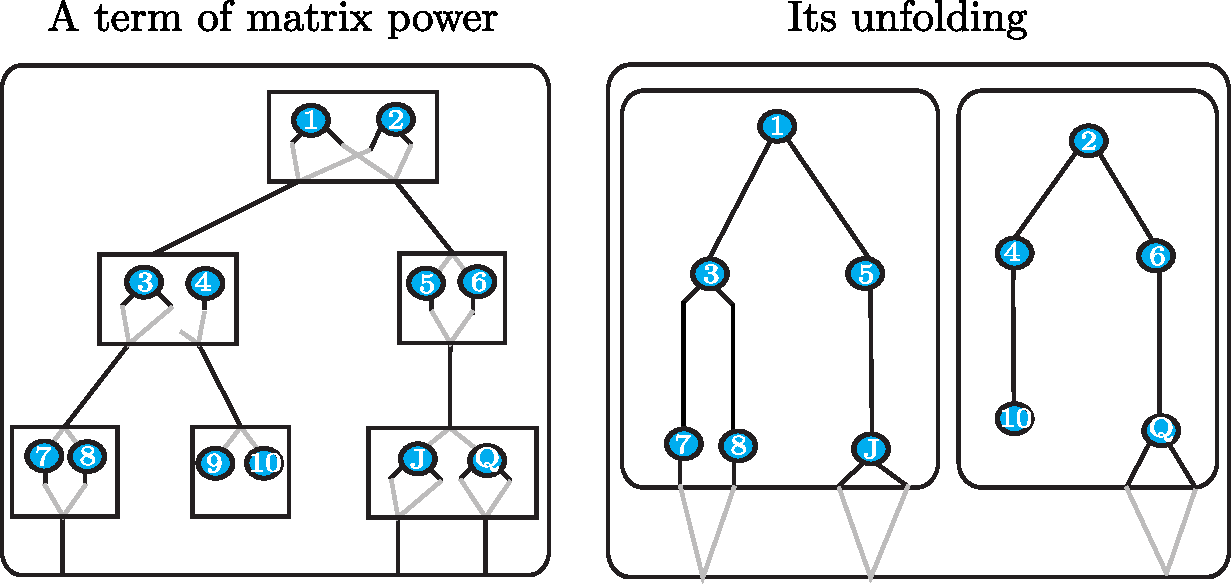
\includegraphics[scale=.38]{unfold-matrix-power}
% % \end{center}
% %  which is defined as follows by induction on the size of the input term. 
% If the input is an empty term, then the output is this term:
% \begin{center}
% \includegraphics[scale=.3, page=83]{pics.pdf}
% \end{center}
% % Otherwise, if the input is a nonempty term $(a_1,\ldots,a_k)/f)(t_1,\ldots,t_n)$. 
% Apply unfolding inductively, yielding 
% For $i \in \set{1,\ldots,k}$ define $s_i$ to be the tree where the root label is $a_i$, and the children are obtained ... 

% Consider an edge in the tree $t$, which connects either a node with one of its children, or a node with one of the ports. For $i \in \set{1,\ldots,k}$, define the $i$-th source of the edge to be the node ; likewise define the $i$-th target of the edge to be the $i$-th subnode of $s$.  For a node $x$ in $t$ and $i \in \set{1,\ldots,k}$, define the $i$-th subnode of $x$ to be the label (from $\rSigma$) in the $i$-th coordinate of the label of $x$.  For a subnode, define its \emph{outgoing edge} to be the edge of the tree 

% Define a \emph{inport} of $s$ to be a pair (node of $s$, number in $\set{1,\ldots,k$}). Define an \emph{outport} to be a pair (node $s$, number in $\set{1,\ldots,k}$, number in $\set{1,\ldots,\text{arity of $s$}$}). 

% \begin{align*}
% \underbrace{\text{(nodes in $s$)} \times \set{1,\ldots,k}}_{\text{sub-nodes}} 
% \qquad
% \underbrace{\text{(edges in $s$)} \times \set{1,\ldots,k}}_{\text{sub-edges}}
% \end{align*}
% For a sub-node $(v,i)$, define its label to be the label in $\rSigma$ of the $i$-th coordinate in the label of $v$. Define the arity of the sub-node to be the arity of its label. If a sub-node has arity $n$, and $j \in \set{1,\ldots,n}$, then the $j$-th out-going sub-edge of the sub-node is defined in the natural way. 


% Consider an  element
% \begin{align*}
% (a_1,\ldots,a_k)/f  
% \end{align*}

% \begin{align*}
% \coprod_{i \in \set{1,\ldots,k}} \set{1,\ldots,\text{arity of $a_i$}} \qquad \to \qquad \set{1,\ldots,n} \times \set{1,\ldots,k}
% \end{align*}
% For $i \in \set{1,\ldots,k}$ and a node node $v$ in the tree $s$ which has label $(a_1,\ldots,a_k)/f$. For $j \in \set{1,\ldots,\text{arity of $a_i$}}$. Let define the $j$-th child of to be the 

% Define a \emph{sub-edge} to be a pair (edge in $s$, number in $\set{1,\ldots,k}$). Define a \emph{sub-node} to be a pair (node in $s$, number in )

% then the output is obtained by first applying unfolding to to the smaller terms $t_1,\ldots,t_n$, and then applying the following derivable function, which we call \emph{shallow unfold}. 
% \begin{align*}
%     \ranked{
%         \xymatrix{
%             \shallowterm{\mati k \rSigma} {\mati k \rGamma}  \ar[r] & \mati k {(\shallowterm \Sigma \Gamma)}.
%         }
%     }
% \end{align*}
% Here is a picture of unfolding for shallow terms:
% \begin{center}
% 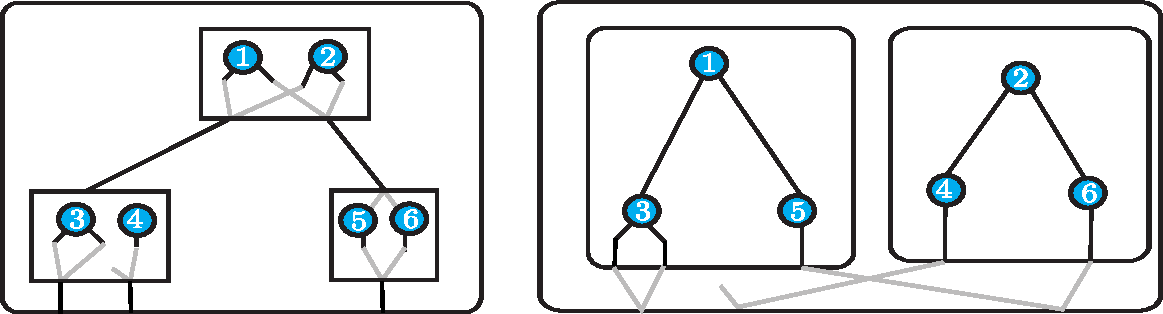
\includegraphics[scale=.4]{unfold-shallow}
% \end{center}
\bibliographystyle{plain}
\bibliography{bib}

\appendix
\section{Examples of derivable functions}\label{sec:AppendixExamples}
To illustrate derivable functions, we present a series of examples, some of them will be useful later.


\noindent \begin{example}[Tree homomorphisms]\label{ex:morphism} 
Given two types $\rSigma, \rGamma$ and an arity preserving  function $\ranked{f:\Sigma\to\tmonad\Gamma}$, we can lift $\ranked{f}$ to the tree homomophism  $\ranked{\mathsf{Hom}_f:\tmonad\Sigma\to \tmonad\Gamma}$ which replaces every node by the term corresponding to its label. If $\ranked{f}$ is derivable, then so is  $\ranked{\mathsf{Hom}_f}$. To see this, we use the composition of the two basic functions
\begin{align*}
\ranked{\tmonad\Sigma\xrightarrow{\tmonad f}\tmonad\tmonad\Gamma \xrightarrow{\flatt_\Gamma} \tmonad \Gamma}
\end{align*}
\end{example}

\noindent\begin{example}[Filter]\label{ex:filter} Consider the types $\rGamma, \rSigma$  where $\rGamma$ is a finite type of unary symbols. Consider the function:
$$ \ranked{f:\tmonad (\rSigma+\rGamma)\to\tmonad \rSigma}$$
which erases the elements of $\rGamma$ from the input term. This function is well defined since erasing unary symbols does not break the tree structure of the input.
Let us explain why this is a derivable function.
Consider the basic functions $\ranked{\unit_\rSigma:\rSigma\to\tmonad\rSigma}$ and the constant function $\ranked{\mathsf{empty}:\rGamma\to\tmonad\rSigma}$ which associates to every element of $\rGamma$ the empty term. We compose the following two functions 
\begin{align*}
\xymatrix{
    \ranked{\rSigma+\rGamma}\quad \ar[r]^-{\ranked{\unit_\Sigma+\mathsf{empty}}} & \quad \ranked{\tmonad\rSigma+\tmonad\rSigma}\ar[r]^-{\ranked{\mathrm{forget}}} &\tmonad\rSigma
},
\end{align*}
Then we lift the obtained function to terms, and compose the result with the $\flatt$ function to obtain our function $\ranked{f}$.  
\end{example}

\noindent \begin{example}[Parent and children]\label{ex:sibling}  Let $\rGamma$ be a finite type. We define $\ranked{\rGamma_0}$  to be the ranked set obtained from $\rGamma$ by setting the arity of every element to $0$.  
\medskip
Consider the function:
$$\ranked{ \mathsf{Parent}: \tmonad \rGamma \to \tmonad (\rGamma\otimes (\rGamma_0+0))}$$
which adds to every node of a term in $\tmonad \rSigma$ the label  of its parent if it has one, and $0$ if it is the root.

% from  $(\rGamma\cup\bot)^{\leq n}$, whose lenght is the arity of the node, and such that the $i^{th}$ element of the  list is the symbol of its $i^{th}$ sibling if it has one, otherwise it is $\bot$.
Let us explain how $\ranked{\mathsf{Parent}}$ can be derived. To illustrate this construction, we use the following term over the alphabet $\ranked{\set{1+2+3}}$ as a running example.
\begin{center}
		 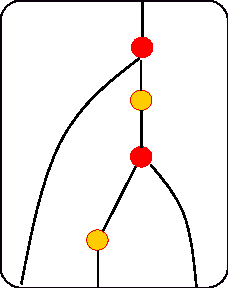
\includegraphics[scale=.6]{parent-1.pdf}
		\end{center}
We denote by $\ranked{\Gamma_1}$ the ranked set obtained from $\rGamma$ by setting the arity of every element to $1$. If $a$ is a element of $\rGamma$, we denote by $a_1$ the corresponding element of $\ranked{\Gamma_1}$. In our example, the alphabet $\ranked{\Gamma_1}$ is
\begin{center}
		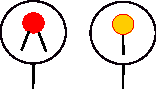
\includegraphics[scale=.5]{parent-2.pdf}
		\end{center}
\begin{enumerate}
\item  First, we apply the homomorphism 
\begin{align*}
\ranked{\mathsf{Hom}_g:\tmonad\Gamma\to \tmonad(\Gamma+\Gamma_1+1)}
\end{align*}
where $\ranked{g}$ is defined on the elements of $\rGamma$ as follows
\begin{align*}
\ranked{g: \Gamma} & \ranked{\to  \tmonad(\Gamma+\Gamma_1+1 )}\\
      a & \mapsto a\tensorpair{1\tensorpair{a_1\tensorpair{0}},\dots, 1\tensorpair{a_1\tensorpair{0}}}
\end{align*}
In our example, the action of $\ranked{g}$ on the elements of $\rGamma$ looks like this
\begin{center}
		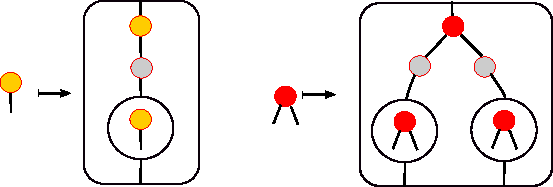
\includegraphics[scale=.5]{parent-3.pdf}
				\end{center}
Hence, after the application of the homomorphism $\ranked{\mathsf{Hom}_g}$, our initial term becomes
\begin{center}
		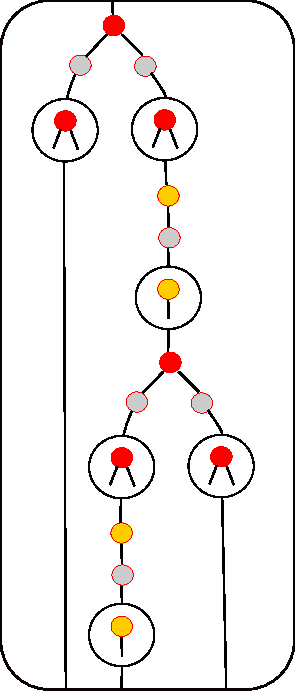
\includegraphics[scale=.5]{parent-4.pdf}
		\end{center}
\item We apply the factorization 
\begin{align*}
\ranked{\ancfact: \tmonad(\Gamma+\Gamma_1+1) \to \tmonad(\tmonad(\Gamma+\Gamma_1)+\tmonad 1)}
\end{align*}
 to separate the symbol $1$ form the other symbols. After this operation, each node lies in the same factor as (the element of $\ranked{\Gamma_1}$ representing) its parent. In our example, the obtained term is the following
\begin{center}
		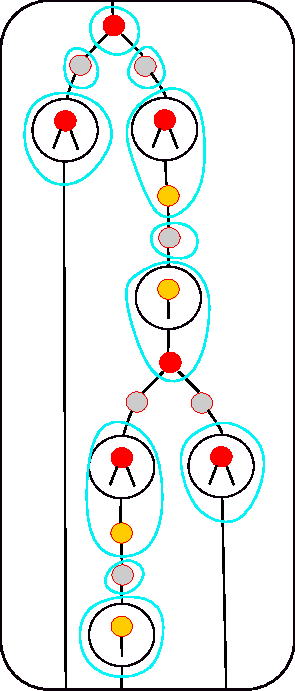
\includegraphics[scale=.5]{parent-5.pdf}
		\end{center}
\item Consider the function 
\begin{align*}
\ranked{h: \tmonad 1 \to \tmonad((\Gamma+\Gamma_1)\otimes(\Gamma_0+0))}
\end{align*}
which is the empty term constant function. It is derivable by lifting the empty term constant function over $1$ to terms.
And let $k$ be the function
\begin{align*}
\ranked{k: \tmonad(\Gamma+\Gamma_1) \to \tmonad((\Gamma+\Gamma_1)\otimes(\Gamma_0+0))}
\end{align*}
which is the identity function, except for the following terms in which it is defined as follows
$$\begin{array}{rll}
a\tensorpair{0,\dots, 0}& \mapsto & \tensorpair{a,0}\tensorpair{0,\dots,0}\\
b_1\tensorpair{a\tensorpair{0,\dots,0}}&\mapsto& \tensorpair{a,b_0}\tensorpair{0,\dots,0}\\
b_1\tensorpair{0} &\mapsto& 0
\end{array}$$
\end{enumerate}
We apply the function $\ranked{h}$ to the factors $\ranked{\tmonad 1}$ and the function $\ranked{k}$ to the factors $\ranked{\tmonad(\rGamma+\rGamma_1)}$. Doing so, we obtain a term in $\ranked{\tmonad\tmonad((\Gamma+\Gamma_1)\otimes(\Gamma_0+0))}$, which we flatten, then we erase the symbols $\ranked{\Gamma_1}$ using the function $\mathsf{Filter}$ of Example~\ref{ex:filter} to obtain the desired term. 
	

\smallskip
If $\rGamma$ is a finite ranked set, we define $\ranked{\Gamma^*}$ as
$$\coprod_{i \leq \text{ maximal arity in } \rGamma} \underbrace{\ranked{\rGamma\otimes \cdots \otimes \rGamma}}_{i\text{ times}}$$
Now consider the function $$\ranked{\mathsf{Children}:\tmonad\rGamma\to \tmonad (\rGamma\otimes (\rGamma_0+0)^*)}$$ which tags every node of a term in $\tmonad \rGamma$ by the list  of its children symbols. When a child is a port, it is marked by $0$ in the list.
The function $\ranked{\mathsf{Children}}$ can be derived using a similar construction as above.
\end{example}



\noindent  \begin{example}[Root and leaves] Let $\rSigma$ be a finite type and $\ranked{f:\rSigma \to \rGamma}$, $\ranked{g: \rSigma \to \rGamma}$ be derivable functions. The function $$\ranked{\mathsf{Root}_{f,g} : \tmonad\rSigma \to \tmonad\rGamma}$$
which applies $\ranked{f}$ to the root and $\ranked{g}$ to the rest of the tree is a derivable function.
To show this, we first start by applying the function $\ranked{\mathsf{Parent}}$. Doing so, the root can be distinguished from the other nodes since it will be tagged by $0$.  

The function $\ranked{h}$ defined below is derivable since its domain is finite. 
\begin{align*}
\ranked{h:\rSigma\otimes(\rSigma_0+0)}&\ranked{\to \rGamma}\\
  \tensorpair{a,0} &\mapsto f(a) \\
  \tensorpair{a,b} &\mapsto g(a) \text{ if } b\neq 0.
\end{align*}
We lift $\ranked{h}$ to terms to conclude.

\smallskip
Similarly, the function $$\ranked{\mathsf{Leaves}_{f,g} : \tmonad\rSigma \to \tmonad\rGamma}$$
 which applies $\ranked{f}$ to the leaves and $\ranked{g}$ to the rest of the tree is derivable. This is done using the same ideas as before, but invoking the function $\ranked{\mathsf{Children}}$ instead of the function $\ranked{\mathsf{Parent}}$: leaves can be distinguished from the other nodes since they are tagged either by a list of $0$ or the empty list.
\end{example}


\noindent\begin{example}[Descendants and ancestors]\label{ex:descendant} If $\rSigma$ is a finite type and $\rGamma\subseteq \rSigma$, then the functions 
\begin{itemize}
\item $\ranked{\mathsf{Descendant}_\rGamma: \tmonad \rSigma \to \tmonad (\rSigma+\rSigma)}$ which replaces the label of each node by its first or second copy, depending on whether it has a descendant in $\rGamma$,
\item $\ranked{\mathsf{Ancestor}_\rGamma: \tmonad \rSigma \to \tmonad (\rSigma+\rSigma)}$ which replaces the label of each node by its first or second copy, depending on whether it has a descendant in $\rGamma$,
\end{itemize}
are derivable.

To derive $\ranked{\mathsf{Descendant}_\rGamma}$, we start by applying the factorization $$\ranked{\decfact: \tmonad\rSigma\to \tmonad(\tmonad\rGamma+\tmonad(\rSigma\setminus\rGamma))}$$ which regroups the elements of $\rSigma$ and the elements of $\ranked{\rSigma\setminus\rGamma}$ into factors depending on whether they have the same ancestors of the same type.

% as in the following figure, where $\rGamma$ is represented by the blue nodes and $\ranked{\rSigma\setminus \rGamma}$ by the yellow ones:
%\begin{center}
%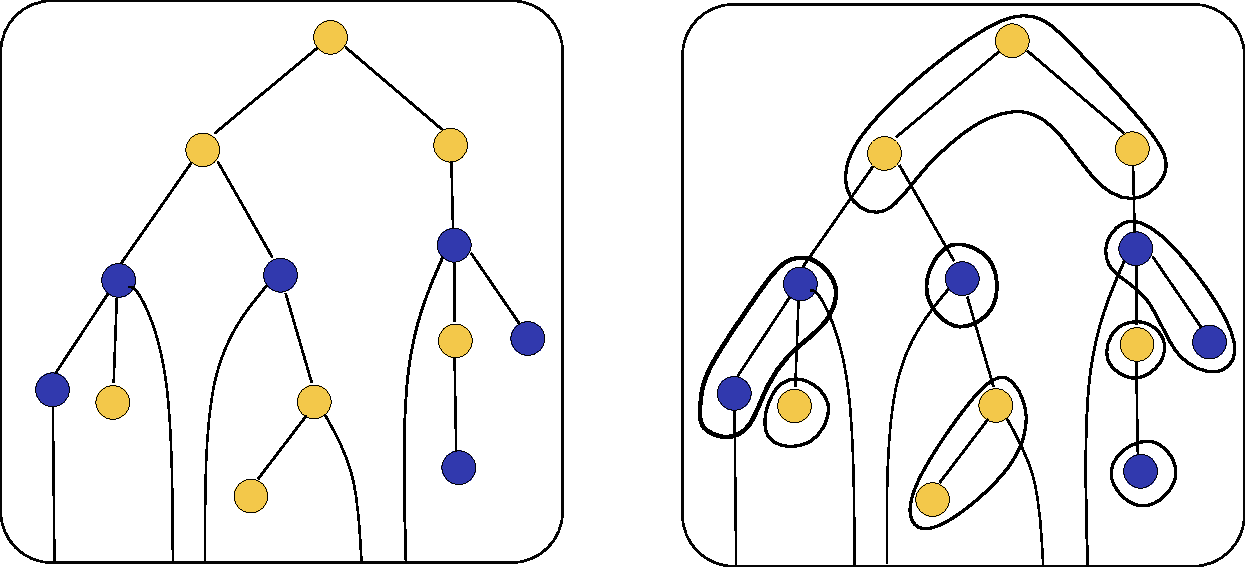
\includegraphics[scale=.3]{descendant.pdf}
%\end{center}
Obviously, all the nodes of the $\rGamma$ factors have a descendant in $\rGamma$. 
In the $\ranked{\rSigma\setminus\rGamma}$ factors which are not leaves in the factorized term, all the nodes have a $\rGamma$ descendant in the original term. To show this, take $f$ to be one of these factors, and suppose by contradiction that one of its nodes does not have a descendant in $\rGamma$. By definition of $\ancfact$, all the elements of $f$ do not have a descendant in $\rGamma$ as well. Since $f$ is not a leaf, it has a child $g$. The factor $g$ cannot be a $\rGamma$
factor as the nodes of $f$ would have a descendant in $\rGamma$. The factor $g$ is then necessarily  a $\ranked{\rSigma\setminus \rGamma}$ factor. If a node of $g$ has a descendant in $\rGamma$, this would give a $\rGamma$ descendant to one of the node of $f$. Thus all the nodes of $g$ are in $\ranked{\rSigma\setminus \rGamma}$ and do not have a descendant in $\rGamma$, meaning that $f$ and $g$ are actually the same factor, which gives a contradiction. Finally, the $\ranked{\rSigma\setminus\rGamma}$ factors which are leaves do not have a descendant in $\rGamma$. With these observations, we can now implement $\mathsf{Descendant}_\rGamma$. 

Let us consider the functions 
$$\begin{array}{llll}
\ranked{\mathsf{Yes}_\rGamma :} & \rGamma &\ranked{\to} &\ranked{ \rSigma+\rSigma}\\
 \ranked{\mathsf{Yes}_{\ranked{\rSigma\setminus\rGamma}:}}& \ranked{\rSigma\setminus\rGamma}&\ranked{\to} &\ranked{ \rSigma+\rSigma}\\
\ranked{\mathsf{No}_{\ranked{\rSigma\setminus\rGamma}: }}&\ranked{\rSigma\setminus\rGamma} &\ranked{\to}& \ranked{ \rSigma+\rSigma}
\end{array}$$
which replaces the label of each node by its first copy for $\ranked{\mathsf{Yes}_\Gamma}$ and $\ranked{\mathsf{Yes}_{\rSigma\setminus\rGamma}}$, and by its second copy for $\ranked{\mathsf{No}_{\rSigma\setminus\rGamma}}$. The three functions are derivable as their domains are finite. 
Consider the functions 
\begin{align*}
\ranked{f:=} &\ranked{ \tmonad\mathsf{Yes}_\rGamma +\tmonad\mathsf{No}_{\rSigma\setminus \rGamma}}\ranked{: \tmonad\rGamma+\tmonad(\rSigma\setminus\rGamma) \to \tmonad (\rSigma+\rSigma)}
\\
\ranked{g:=} & \ranked{ \tmonad\mathsf{Yes}_\rGamma
+\tmonad\mathsf{Yes}_{\rSigma\setminus \rGamma}}\ranked{: \tmonad\rGamma+\tmonad(\rSigma\setminus\rGamma) \to \tmonad (\rSigma+\rSigma)} 
\end{align*}
The descendant function is obtained by applying $\ranked{\mathsf{leaves}_{f,g}}$ followed by a flattening.

\smallskip
To derive the function $\ranked{\mathsf{Ancestor}_\Gamma}$, we apply first a the factorization
\begin{align*}
\ranked{\ancfact: \tmonad\rSigma\to \tmonad(\tmonad\rGamma+\tmonad(\rSigma\setminus\rGamma))}
\end{align*} which regroups the elements of $\rSigma$ and the elements of $\ranked{\rSigma\setminus\rGamma}$ into factors depending on whether they have the same descendants of the same type. 
Using similar arguments as before, we can conclude that:
\begin{itemize}
\item The nodes inside $\rGamma$ factors have $\rGamma$ ancestors.  
\item If a $\ranked{\rSigma\setminus\rGamma}$ factor is the root of the factorized term, then its nodes do not have a $\rGamma$ ancestor.
\item   If a $\ranked{\rSigma\setminus\rGamma}$ factor is not the root of the factorized term, then its nodes do have a $\rGamma$ ancestor.
\end{itemize}
The ancestor function is obtained by applying $\ranked{\mathsf{root}_{f,g}}$ followed by a flattening.
\end{example}




\section{Derivable functions can be described in first-order logic}
\label{sec:to-logic}
We show in this section that derivable functions can be implemented by first-order transductions. 
Let us start be defining the function 
\begin{definition}[Associated models for terms, pairs, co-pairs and tensors.] \label{def:type-model} To each type  $\rSigma$ we associate a vocabulary, called the \emph{vocabulary of $\rSigma$}, and a map 
    \begin{align*}
        a \in \rSigma \qquad \mapsto \qquad \underbrace{\underline a \in \text{models over the  vocabulary of  $\rSigma$}}_{\text{associated model of $a$}}.
    \end{align*}
    Furthermore, for each $a \in \rSigma$ we  distinguish a  sequence (whose length is the arity of $a$) of elements in $\underline a$, which are called the ports of $\underline a$.   The definitions are by induction on the structure of $\rSigma$, as given below.
    \begin{itemize}
        \item \emph{Finite ranked sets.} Elements of a ranked set   \begin{align*}
        \rSigma =  \set{a_1,\ldots,a_k}
        \end{align*} are modeled  using a vocabulary which has unary relations $a_1,\ldots,a_k$ and $P_1,\ldots,P_m$ where $m$ is the maximal arity of elements in $\rSigma$. 
        For $a \in \rSigma$ of arity $n$, the  universe of $\underline a$ is $\set{0,1,\ldots,n}$, with the ports being $1,\ldots,n$. 
            The  relation $P_i$  is interpreted as $\set i$ when $i \in \set{1,\ldots,n}$ and as the empty set otherwise. The relation $a_i$ is interpreted as $\set 0$ when $a = a_i$ and as the empty set otherwise. 
        \item \emph{Coproduct.}  Elements of the coproduct $\ranked{\Sigma_1 + \Sigma_2}$ are modeled using the disjoint union of the vocabularies of $\ranked{\Sigma_1}$ and $\ranked{\Sigma_2}$. 
            If an element of the coproduct comes from $\ranked{\Sigma_1}$, then its associated model is defined as for the type $\ranked{\Sigma_1}$, with  the remaining relations from the vocabulary of   $\ranked{\Sigma_2}$ interpreted   as empty sets. The definition is analogous for  elements from $\ranked{\Sigma_2}$. 
        \item \emph{Tensor product.}   Tensor pairs in   $\ranked{\Sigma_1 \otimes \Sigma_2}$ are modeled
        using the disjoint union of the vocabularies of $\ranked{\Sigma_1}$ and $\ranked{\Sigma_2}$. 
            For  $\tensorpair{a_1,a_2}$, the associated model is    the disjoint union $\underline{a_1} + \underline {a_2}$, with the relations of $\underline {a_1}$ using the  vocabulary of ${\ranked{\Sigma_1}}$, and the relations of $\underline {a_2}$ using the vocabulary  ${\ranked{\Sigma_1}}$. 
            If $n_1$ is the arity of $a_1$, then the first $n_1$ ports are inherited from  $\underline {a_1}$ and the remaining ports are inherited from  $\underline {a_2}$.
        \item \emph{Cartesian product.}   Cartesian pairs in  $\ranked{\Sigma_1 \otimes \Sigma_2}$ are modeled  using the disjoint union of the vocabularies of $\ranked{\Sigma_1}$ and $\ranked{\Sigma_2}$, plus an extra binary relation $R$.  
            The model associated to a Cartesian pair   $ (a_1,a_2)$,  is      the disjoint union $\underline{a_1} +  \underline {a_2}$, in the same sense as in the previous item for $\otimes$,  with the binary relation $R$ interpreted as 
                \begin{align*}
                   \quad \set{(\text{$i$-th port of $\underline {a_1}$}, \text{$i$-th port of $\underline a_2$}): i \in [1,\text{arity of $(a_1,a_2)$}]} 
                \end{align*}
                The ports are inherited from   $\underline {a_1}$.
        \item \emph{Folding.}   For $k \in \set{1,2,\ldots}$, elements of   $\reduce k \rSigma$ are modeled using the  vocabulary of $\rSigma$ plus two extra binary relations $\portord$ and $R$. If $a \in \rSigma$ has arity $nk$, then the model associated to $a/f$ -- which has arity $n$ --   is obtained from  $\underline{a}$ by adding a copy of the model below, where $\sqsubset$ is the natural ordering on integers
                \begin{align*}
                (\set{1,\ldots,n}, \portord),
                \end{align*}
whose elements are used as the ports, and interpreting the binary relation $R$ as
        \begin{align*}
        \set{(\text{$i$-th port of $\underline a$},f(i)) : i \in \set{1,\ldots,nk}}
        \end{align*}
                
                
        \item \emph{Terms.}   Terms in $\tmonad \rSigma$ are modeled using vocabulary of $\rSigma$ extended with two fresh binary relations $\anceord$ and $\portord$. 
          Let $t \in \tmonad \rSigma$. Consider the disjoint union of models
            \begin{align}\label{eq:non-port}
                 \coprod_{x \in \text{non-port nodes in $t$}} \underline{a(x)},
            \end{align}
         where  $\underline a(x)$ is the model over vocabulary of $\rSigma$ that  is defined by induction assumption.   In the above  disjoint union, the same vocabulary, namely the vocabulary of $\rSigma$,  is used  for all parts of the disjoint union. Next, consider  the model
            \begin{align}\label{eq:ports}
            (\set{1,\ldots,n}, \portord)
            \end{align}
            where $\portord$ is the natural ordering on $\set{1,\ldots,n}$. 
            The model of $t$ is defined by taking the disjoint union of the models in~\eqref{eq:non-port} and~\eqref{eq:ports}, and defining the descendent relation $\anceord$ as the set of pairs $(u,v)$ such that:
            \begin{itemize}
            \item either $u$ is the $i$-th port of $\underline{a(x)}$ for some node $x$ of $a$, $v$ is a port of $\underline{a(y)}$ for some node $y$ which is a descendent of the $i$-th child of $x$.
            \item or $u$ is the $i$-th port of $\underline{a(x)}$ for some node $x$ of $a$, $v=j\in\{1,\dots,n\}$ and the $j$-th port of $a$ is a descendent of the $i$-th child of $x$.
            \end{itemize} 

            % It  consists of all pairs $(u,v)$ such that $u$ is the $i$-th port of $\underline{a(x)}$  some non-port node $x$, and $v$ belongs to $\underline{a(y)}$ for some node (possibly a port) $y$ which is a descendant (not necessarily proper) of the $i$-th child of $x$. The binary relation $\portletter$ is the total order 
           % The ports are taken from the structure~\eqref{eq:ports}.
    \end{itemize}
\end{definition}

The above  definition creates a certain ambiguity for trees, because if $t$ is a tree over a finite ranked set $\rSigma$, then $\underline t$ can be understood in two ways: as per  Definition~\ref{def:tree-model} for trees, or as per Definition~\ref{def:type-model} when $t$ is viewed as a special case of a term $t \in \tmonad \rSigma$. Since we only use first-order transductions to transform relational structures,  this ambiguity is not a problem, because one can easily define first-order transductions which map one definition of $\underline t$ to the other.



The proof proceeds by induction, following the definition of derivable functions. All the cases are easy, and consist mainly on unfolding the definitions. We will treat only the cases of the basic function $\unit_\rSigma$  to illustrate this process.
    
    In the following, it will be convenient to use, as part of the vocabulary of $\rSigma$, the unary relation  $\mathsf{Port}_\rSigma$ which selects the ports of the structures over the vocabulary of $\rSigma$; and the binary relation $\sqsubset_\rSigma$ which orders these ports. By induction on $\rSigma$, we can show that both relations are definable by first-order formulas over  the vocabulary of $\rSigma$.
    
    
   Given an element $x$ of $\rSigma$, let us show how  $\unit_\rSigma(x)$ can be implemented using a FO transduction.  The copying constant is 2,
    the first copy will contain the whole structure $\underline{x}$ and the second copy will select only the ports of $\underline{x}$ which will serve as the ports of the structure $\underline{\unit_\rSigma(x)}$, as illustrated by the following picture 
\begin{center}
    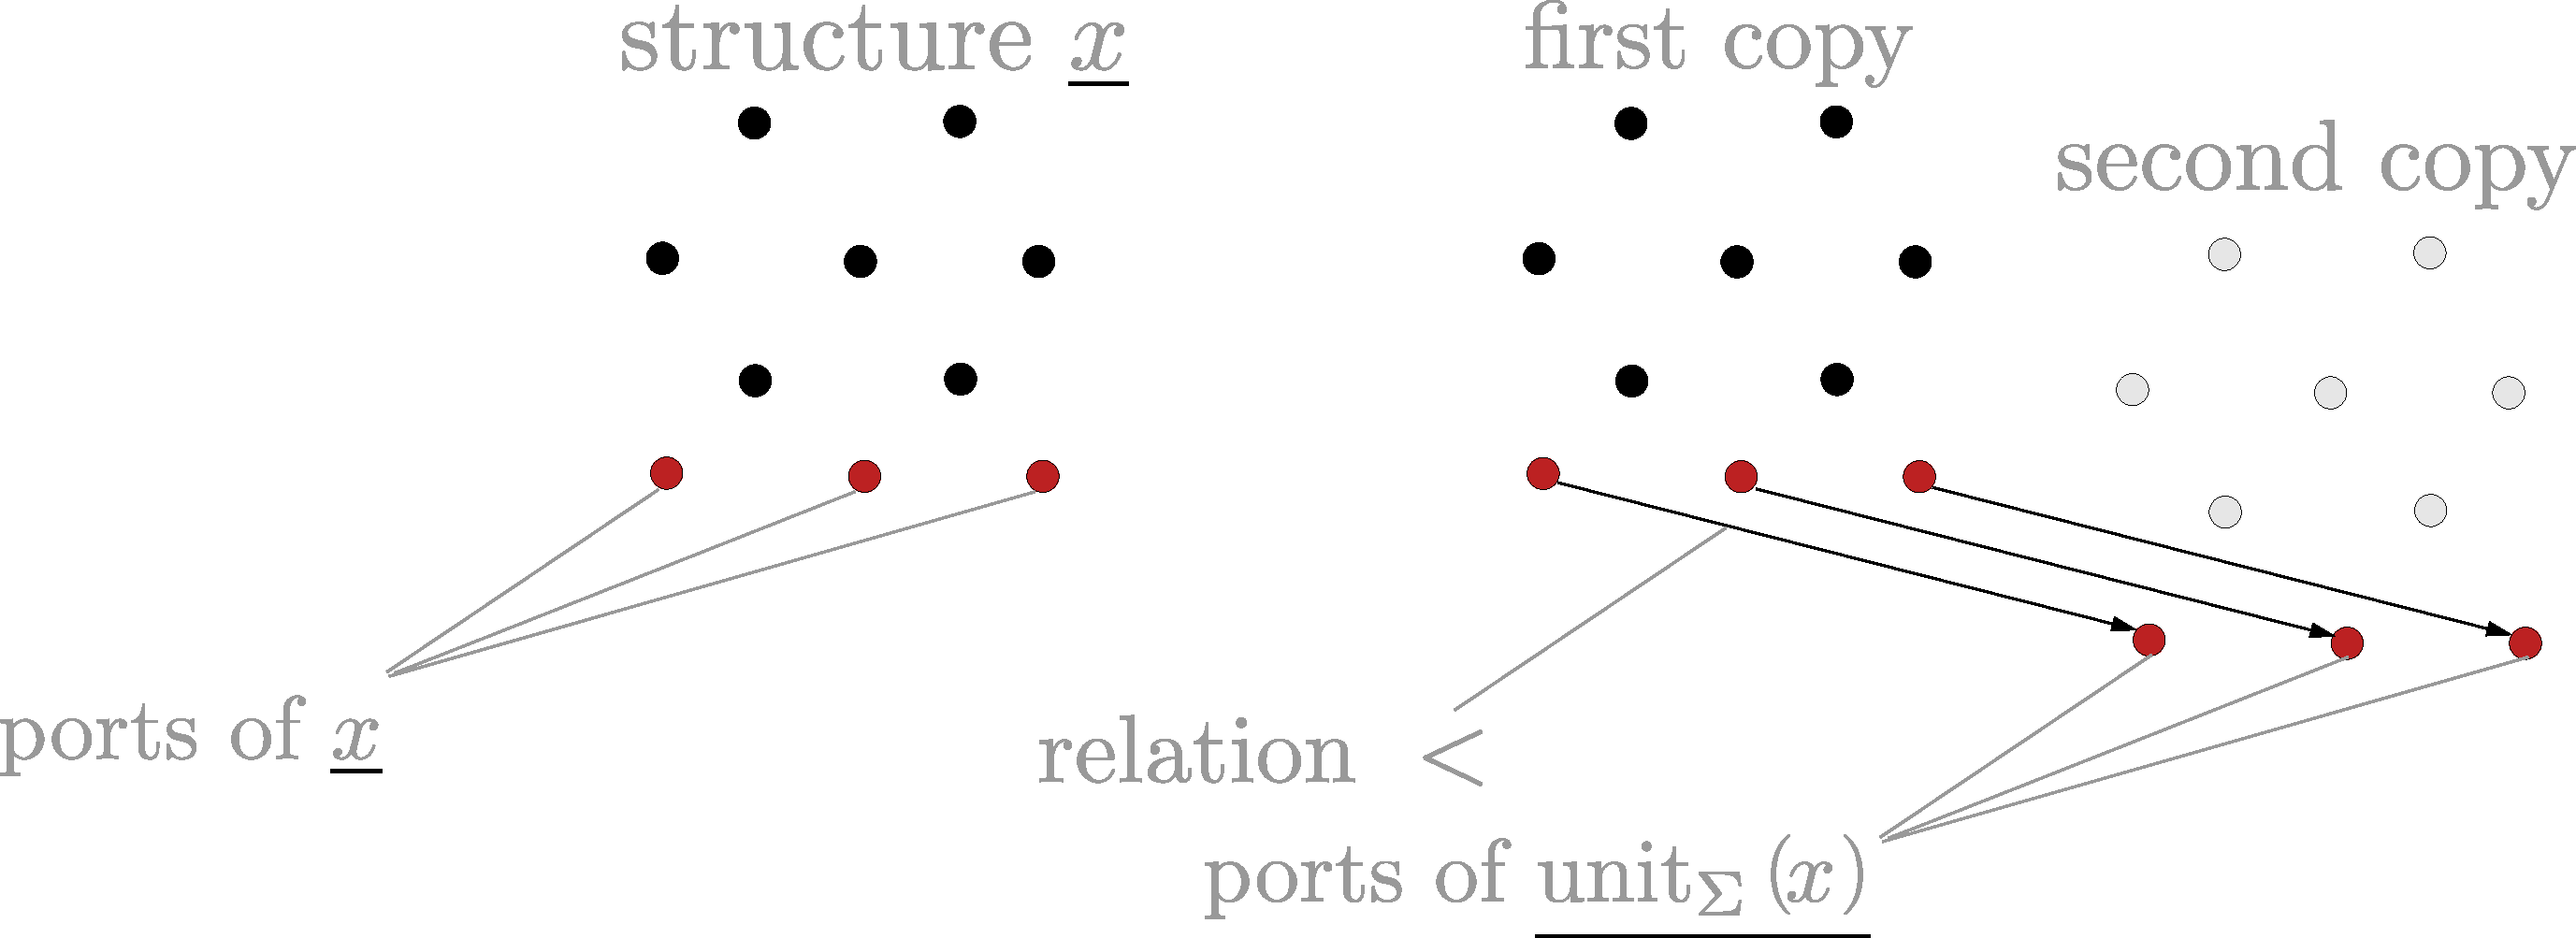
\includegraphics[scale=.18]{pictures/to-logic-unit.pdf}
    \end{center}    
      The universe formulas are then:
    \begin{align*}
    \varphi_1(x)=\mathsf{True} \qquad \varphi_2(x)=\mathsf{Port}_\rSigma(x)
    \end{align*}
    In the first copy, the vocabulary of $\rSigma$ will be interpreted as in the original structure, and as the empty set in the second copy. That is, for every unary relation $R$ and for every binary relation $S$ in the vocabulary of  $\rSigma$, we set:
    \begin{align*}
   \varphi_R^{1}(x)=R(x) \quad&\quad \varphi_S^{1,1}(x,y)=S(x,y)\\
   \varphi_R^{2}(x)=\mathsf{False} \quad&\quad \varphi_S^{2,2}(x,y)=\mathsf{False}
\end{align*}      
Let us interpret the relations $<$ and $\sqsubset$ of the vocabulary of $\tmonad\rSigma$. The  ports of $\underline{\unit_\rSigma(x)}$ inherit the order of the ports of $\underline{x}$, this is why we set:
\begin{align*}
\varphi_\sqsubset^{2,2}(x,y)=x\sqsubset_\rSigma y
\end{align*}
The descendant relation $<$ connects the $i^{th}$ port of $\underline{x}$ to the $i^{th}$ port of $\underline{\unit_\rSigma(x)}$. Since these nodes come from the same node in the original structure, we set:
\begin{align*}
\varphi_<^{1,2}(x,y)=x=y
\end{align*}
\section{Appendix on first-order relabelling}~\label{sec:AppendixForat}


\subsection{Reduction to Schilgloff's theorem}

In this section, we provide more details about the proof of Lemma~\ref{lem:schlingloff}. We recall its statement below.

\begin{lemma} \label{restatelem:Schlingloff}The first-order tree relabeling are equal to the smallest class of functions which is closed under composition and which  contains the following functions:
    \begin{enumerate}
        \item \label{it:relabeling} \emph{Relabeling}. To every finite $\rGamma,\rSigma$ and $\ranked {f : \rSigma \to \rGamma}$, the tree lifting $\trees \ranked f : \trees \rSigma \to \trees \rGamma$.
        \item \label{it:child} \emph{Child.} For every $\rSigma$ and  $i \in \set{1,2,\ldots}$, the characteristic function of the  unary query 
        \begin{align*}
            \underbrace{\child i (x).}_{\text{$x$ is an $i$-th child}}
        \end{align*}
         \item \label{it:until} \emph{Until.} For every finite $\rGamma, \rDelta \subseteq \rSigma$,  the characteristic function of the unary query
         \begin{align*}
              \underbrace{\exists y\ y > x \land \rDelta(y) \land  \forall z \ (x < z < y \Rightarrow \rGamma(z)).}_{\substack{\text{$x$ has a descendant $y$ with label in $\rDelta$, such that}\\ \text{all nodes strictly between $x$ and $y$ have label in $\rGamma$}}} 
         \end{align*} 
         \item \label{it:since}\emph{Since.} For every $\rGamma, \rDelta \subseteq \rSigma$,    the characteristic function of the unary query
         \begin{align*}
              \underbrace{\exists y\ y < x \land \rDelta(y) \land  \forall z \ (y < z < x \Rightarrow \rGamma(z)).}_{\substack{\text{$x$ has a descendant $y$ with label in $\rDelta$, such that}\\ \text{all nodes strictly between $x$ and $y$ have label in $\rGamma$}}}  
         \end{align*} 
    \end{enumerate}
    In items \ref{it:child} -- \ref{it:since}, the alphabet is $\rSigma$, so the characteristic functions have type $\trees \rSigma \to \trees(\rSigma + \rSigma)$. 
\end{lemma}
Clearly the functions in the lemma are first-order tree relabelings, and first-order tree relabelings are easily seen to be closed under composition, which gives the right-to-left inclusion in the lemma. The hard part is the left-to-right inclusion, which says that every first-order tree relabeling can be decomposed into functions as in items~\ref{it:relabeling} -- \ref{it:since}. 
The first  step in the proof of  the right-to-left inclusion is the observation that  every first-order tree relabeling can be decomposed as 
\begin{align*}
    g \circ f_1 \circ \cdots \circ f_n
\end{align*}
where $g$ is a relabeling as in item~\ref{it:relabeling} of the lemma and each $f_i$ is a  characteristic function of some unary query (not necessarily of the simple form indicated in items~\ref{it:child} -- \ref{it:since} in the lemma). This is a simple observation: the functions $f_1,\ldots,f_n$ annotate the tree with the truth values of the unary queries used in the definition of the  first-order relabeling, and $g$ uses these truth values to select the appropriate output label. The hard part of the lemma is showing that each $f_i$  can be further decomposed into functions as indicated in the lemma. This is where we us the result of Schlingloff~\cite[Theorem 2.6]{schlingloff1992expressive}, which says that all first-order definable tree properties can be defined using a temporal logic that has operators similar to the ones used in items~\ref{it:child} -- \ref{it:since} of the lemma. 

The following table summeraizes our framework (first column) and Shcligloff's one (second column). The first row describes the model of trees under consideration, the second row the correponding version of first-order logic, and the third row the correponding temporal logic. 
\begin{center}
\begin{tabular}{C{1.8cm}|C{2.8cm}|C{2.8cm}|}
\cline{2-3}
& {Trees over a ranked alphabet $\rGamma$} & {Models over a set of propositions $P$}\\
\hline 
Description of the model & Finitely branching \footnote{Because $\rGamma$ is finite.} ranked trees, labeled from $\rGamma$. & Finitely branching, unranked trees, labeled from $2^P$. \\
\hline
    \multirow{3}{1.8cm}{First-order logic}&\multicolumn{2}{C{5.6cm}|}{Usual first-order connectives ($\exists, \vee, \neg$) with the descendant predicate $x\leq y$ and the following predicates:}\\
    \cline{2-3} 
                                 & $a(x)$:  $x$ is labeled $a$  $(a \in \rGamma)$.  & $p(x)$: label of $x$ contains $p$
                                  ($p\in P$). \\
                                  &\hspace{-.14cm}$\child i(x)$: $x$ is an $i$-th child. &\\
   &       We call it $\rGamma$-FO.    & We call it $P$-FO.             \\
    \hline
    \multirow{4}{1.8cm}{Temporal logic}& \multicolumn{2}{C{5.6cm}|}{Usual CTL connectives ($S$ (Since), $U$ (Until), $\vee$, $\neg$) together with:}\\
    \cline{2-3} 
    
     & $a \in \rGamma$, & $p \in P$, \\
    & $\odot_i \phi$: the $i$-th child satisfies $\phi$. & $X_i \phi$: at least $i$ children satisfy $\phi$.\\ 
    &       We call it 2-CTL.    & We call it 4-CTL.             \\
    \hline
\end{tabular}
\end{center}

Schlingloff's theorem says that P-FO formulas are equivalent to 4-CTL formulas. To prove Lemma~\ref{restatelem:Schlingloff}, we need to prove that $\rGamma$-FO formulas are equivalent to 2-CTL ones. 
For this purpose, we will show how to translate every ranked tree $t$ over $\rGamma$ into a model $[t]$ over a well chosen set of propositions $P$. Then we will apply the following scheme

 
    $$\xymatrix@C=2cm{
        \varphi \in \rGamma\text{-FO} 
        \ar[r]^{\forall t, \ t\models \varphi \ \leftrightarrow \ [t] \models \psi}_{\text{Lemma}~\ref{lem:from-Gamma-to-P-FO}}
        &
        \psi \in P \text{-FO}
        \ar[d]^{\substack{\text{Schlingloff}\\\text{theorem}}} \\
       \theta \in \text{2-CTL}
        \ar[r]^{\forall t, \ t\models \theta \ \leftrightarrow \ [t] \models \delta}_{\text{Lemma}~\ref{lem:from-4-CTL-to-2CTL}}
        &
        \delta \in \text{4-CTL}
    }$$    

 Let us show the translation $[\_]$ and Lemmas~\ref{lem:from-Gamma-to-P-FO} and \ref{lem:from-4-CTL-to-2CTL}.

\paragraph{From ranked trees to Schlingloff's models.} Let us fix a ranked alphabet $\rGamma$. Let $P$ be the following set of propositions
\begin{align*}
P\eqdef \rGamma\cup\set{i\text{-th-child}\ |\ i\in[1, \text{max arity of }\rGamma]}
\end{align*}
 Let $t$ be a ranked tree over $\rGamma$. The translation $[t]$ of $t$ is the model defined as follows. It has the same set of nodes and the same descendant relation as $t$. The label of a node contains $a$ if its label in $t$ is $a$. It contains the proposition $i\text{-th-child}$ if it is an $i$-th child in $t$.

\paragraph{From $\rGamma$-FO to $P$-FO.} Let $\rGamma$ and $P$ as before. We show that
\begin{lemma}\label{lem:from-Gamma-to-P-FO}
For every $\rGamma$-FO formula $\phi$, there is a $P$-FO formula $\psi$ such that
$$ \forall t\in \trees\rGamma, \qquad t\models \phi \leftrightarrow [t]\models \psi$$
and conversely.
\end{lemma}
\begin{proof}

\end{proof}

\paragraph{From 4-CTL to 2-CTL}
Let $\rGamma$ and $P$ as before. We show that
\begin{lemma}\label{lem:from-4-CTL-to-2CTL}
For every $\rGamma$-FO formula $\phi$, there is a $P$-FO formula $\psi$ such that
$$ \forall t\in \trees\rGamma, \qquad t\models \phi \leftrightarrow [t]\models \psi$$
and conversely. \end{lemma}
\begin{proof}

\end{proof}
%Let $\rGamma$ be a ranked alphabet. The formulas of 2-$\mathsf{CTL}$ are generated by the following syntax:
%\begin{align*}
%\varphi, \psi:= \ a\in \rGamma \ | \ \odot_i \phi \ | \ \varphi\untilmod \psi \ | \ \varphi\sincemod\psi  
%\end{align*}
%The semantics of these formulas are defined for the ranked trees of $\trees \rGamma$ as follows.
%\begin{enumerate}
%\item A tree of $\trees \rGamma$ satisfies the formula $a\in\rGamma$ at the node $x$ if the label of $x$ is $a$.
%\item $t, x\models \odot_i \varphi$ if the $i$-th child of $x$ satisfies $\varphi$.
%\item  The formula $\varphi\untilmod \psi$  is valid  in the node $x$ if $x$ has a descendant $y$ with label in $\rDelta$, such that all nodes between $x$ and $y$ have label in $\rGamma$. 
%\item $x$ has a descendant $y$ with label in $\rDelta$, such tha all nodes between $x$ and $y$ have label in $\rGamma$.
%\end{enumerate}
%
%\begin{lemma}%[Decomposition lemma]
%For every first-ordre formula $\phi$, there is a $2$-$\mathsf{CTL}$ formula $T$ such that
%$$ \forall t\in \trees \rGamma \qquad t,x\models \varphi \Leftrightarrow t,x\models T.$$
%\end{lemma}
%
%Shclingloff considers node labeled, branching bounded and   unordered (there is no order between the children of a node) trees. If $\Gamma$ is an (unranked) alphabet, we denote by $\trees_b\Gamma$ the set of unordered trees, labelled from $\Gamma$ and whose branching is at most $b$.   
%
%
%The formulas of $4$-$\mathsf{CTL}$ are generated by the following syntax:
%\begin{align*}
%\varphi, \psi:= \ a\in \Gamma \ | \ \nextmod_i \phi \ | \ \varphi\untilmod \psi \ | \ \varphi\sincemod\psi  
%\end{align*}
%The semantics of $4$-$\mathsf{CTL}$ formulas is as before. The connective $\nextmod_i$ have the following semantics:
%%
%%\begin{theorem}\cite{}%[Decomposition lemma]
%%For every first-ordre formula $\phi$, there is a $4$-$\mathsf{CTL}$ formula $T$ such that
%%$$ \forall t\in \trees_b \Gamma \qquad t,x\models \varphi \Leftrightarrow t,x\models T.$$
%%\end{theorem} 
%% Let us explain how Lemma~\ref{} can be derived from Theorem~\ref{}. First Comment plonger les arbres de $\trees \rGamma$ dans le framework de Schlingloff. Soit $b$ l'arite maximale des elements de $\rGamma$. On denote par $\overline{\rGamma}$ le (unranked) set underlying $\rGamma$. 
%%Il y a un plongement naturel 
%%$$ \overline{\bullet}: \trees\rGamma \to \trees_b\Gamma$$
%
%\paragraph*{Encoding our trees by Schlingloff's trees}
%\paragraph*{Translating first-order formulas}
%\begin{lemma} Let $\rGamma$ be a ranked set and $\phi$ be a first-order formula.
%\begin{align*}
%\forall t\in \trees \rGamma, \qquad t\models \phi \leftrightarrow t \models [\phi]
%\end{align*} 
%\end{lemma}
%
%\paragraph*{From 4-CLT to 2-CTL}
% \begin{lemma} Let $\rGamma$ be a ranked set and $\phi$ be a first-order formula.
%\begin{align*}
%\forall t\in \trees \rGamma, \qquad t\models \overline{\phi} \leftrightarrow [t] \models \phi
%\end{align*} 
%\end{lemma}
%
\subsection{First-order relabelling are derivable}\label{sec:relabeling}

\begin{lemma}\label{lem:nextmod}
  For every finite $\rSigma$, $\rGamma\subseteq \rSigma$ and $i \in \set{1,2,\ldots}$, the characteristic function $\ranked{f:\tmonad \rSigma\to\tmonad(\rSigma+\rSigma)}$ of the  unary query 
        \begin{align*}
\text{``The }i\text{-th child of }x\text{ is in }\rGamma\text{''}
        \end{align*}
        is derivable.
\end{lemma}
\begin{proof}
To show that $\ranked{f}$ is derivable, we start applying the children function \begin{align*}
\ranked{\mathsf{Children}:\tmonad\rSigma\to \tmonad (\rSigma\otimes (\rSigma_0+0)^*)}
\end{align*} from Example~\ref{ex:sibling} which tags every nodes by the list of its children. Consider the function $g$
$$\begin{array}{rlll}
\ranked{g:}  \ranked{\rSigma\otimes (\rSigma_0+0)^*} &\ranked{\to}& \ranked{\Sigma +\Sigma}&\\
            \tensorpair{a,l}                           &
     \mapsto& \tensorpair{a,1}              &\text{if } l[i]\in\ranked{\rGamma_0}, \\
                    &   \mapsto& \tensorpair{a,2} &\text{otherwise.}   
\end{array}$$
which maps an element of $\rSigma$ tagged by a list to the first copy of $\rSigma$ if the $i$-th element of the list is in $\rGamma$ and to the second copy otherwise. The function $g$ is derivable since its domain is finite.
We finally get $\ranked{f}$ by lifting $\ranked{g}$ to terms.
\end{proof}

\medskip
\begin{lemma}\label{lem:untilmod}
For every finite $\rGamma, \rDelta \subseteq \rSigma$,  the characteristic function $\ranked{f:\tmonad\rSigma\to\tmonad(\rSigma+\rSigma)}$ of the unary query
         \begin{align*}
              \underbrace{\exists y\ y \geq x \land \rDelta(y) \land  \forall z \ (x < z < y \Rightarrow \rGamma(z)).}_{\substack{\text{$x$ has a descendant $y$ with label in $\rDelta$, such that}\\ \text{all nodes between $x$ and $y$ have label in $\rGamma$}}} 
              \end{align*}
is derivable.
\end{lemma}
\begin{proof}
We start by applying the factorization
\begin{align*}
\ranked{\ancfact : \tmonad \Sigma \to \tmonad(\tmonad(\Sigma\setminus(\Gamma\cup\Delta)) +\tmonad(\Gamma\cup\Delta))}
\end{align*}
which decomposes our terms into factors, depending on whether their node labels are in $\ranked{\Gamma\cup\Delta}$ or not. 
Note that the value of a node w.r.t. the until query depends only on the node labels of its factor. %(it is constant equal to $0$ in the case of $\Sigma\setminus(\Gamma\cup\Delta)$ blocks).

The nodes of the $\ranked{\tmonad(\rSigma\setminus(\rGamma\cup\rDelta))}$ factors do not satisfy the query, thus we will apply to them the function $\ranked{\tmonad g}$ obtained by lifting the function 
$$\begin{array}{rrll}
 \ranked{g:}& \ranked{\rSigma\setminus(\rGamma\cup\rDelta)}& \ranked{\to} &\ranked{\rSigma+\rSigma}\\
&a&\mapsto& \tensorpair{a,2}.
\end{array}$$
 
  
Nodes of the $\ranked{\tmonad(\Gamma\cup\Delta)}$  factors satisfy the query if and only if they have a descendant in  $\rDelta$.
Consider the function $\ranked{h}$ obtained by composing the descendant function $\ranked{\mathsf{Descendant}_\Delta}$ from Example~\ref{ex:descendant} with an injection $\ranked{\tmonad(\iota+\iota)}$
\begin{align*}
\underbrace{\ranked{\tmonad(\Gamma\cup\Delta) \xrightarrow{\ranked{\mathsf{Descendant}_\Delta}} \tmonad(\Gamma\cup\Delta+\Gamma\cup\Delta) \xrightarrow{\ranked{\tmonad(\iota+\iota)}}\tmonad(\Sigma+\Sigma)}}_{\ranked{h}}
\end{align*}
Finally, to get the characteristic function $\ranked{f}$, we apply $\ranked{\tmonad{g}}$ to the $\ranked{\tmonad(\Sigma\setminus(\Gamma\cup\Delta))}$ factors and $\ranked{h}$ to the other factors using the co-pairing combinator, then we flat the obtained term. 
\end{proof}


\begin{lemma}\label{lem:sincemod}
For every finite $\rGamma, \rDelta \subseteq \rSigma$,    the characteristic function of the unary query
         \begin{align*}
              \underbrace{\exists y\ y \leq x \land \rDelta(y) \land  \forall z \ (y < z < x \Rightarrow \rGamma(z)).}_{\substack{\text{$x$ has a descendant $y$ with label in $\rDelta$, such that}\\ \text{all nodes strictly between $x$ and $y$ have label in $\rGamma$}}}  
         \end{align*} 
         is derivable.
\end{lemma}
\begin{proof}
The same proof as above, one only needs to replace the use of the function $\ranked{\mathsf{Descendant}_\Delta}$ by that of $\ranked{\mathsf{Ancestor}_\Delta}$, introduced in Example~\ref{ex:descendant}.
\end{proof}

\section{Proof of Theorem~\ref{thm:stt}}
\label{sec:stt-appendix}
In this part of the appendix, we prove Theorem~\ref{thm:stt}, which says that every first-order tree-to-tree transduction is recognised by a register transducer. 

According to Definition~\ref{def:fo-transduction}, a first-order transductions is a composition of any number of functions each of which is either  copying (item 1) or a non-copying first-order transduction (item 2). In other words:
$$\begin{array}{c}
\text{first-order transductions} \\ \eqdef (\text{copying} \cup \text{(non-copying first-order transductions)})^*
\end{array}$$
where the star denotes closure under composition. Although register transducers are closed under composition, this is not very   easy to show directly, and therefore we begin by simplifying the function composition in the definition of first-order transductions.  It is not hard to see that copying commutes with non-copying first-order transductions in the following sense:
\begin{align*}
    \text{copying} \circ  \text{(non-copying first-order transductions)}  \\ \subseteq   \text{(non-copying first-order transductions)} \circ \text{copying}.
    \end{align*}
Furthermore, since the class of copying functions is closed under composition, and the same is true for non-copying first-order transductions, we get the following normal form of first-order transductions:
$$\begin{array}{c}
    \text{first-order transductions} \\=  \text{(non-copying first-order transductions)} \circ \text{copying}.
    \end{array}$$
Therefore, in order to prove Theorem~\ref{thm:stt}, it suffices to show that a register transducer can compute any function which first copies the nodes of the input tree a fixed number of times, and then applies a non-copying first-order transduction. 
% To make notation lighter, we ignore the copying, and only show that register transducers can simulate non copying first-order transductions. The proof with copying follows the same lines. 

For the rest of this section, fix  a tree-to-tree function
\begin{align*}
f : \trees \rSigma \to \trees \rGamma
\end{align*}
which is a composition of first copying (some fixed number of times), followed by a non-copying first-order transduction. We will show that $f$ is computed by some register transducer.  

\newcommand{\origin}[1]{\mathrm{origin}_{#1}}
\newcommand{\orcol}[2]{\mathrm{orcol}_{#1}^{#2}}
In the proof, we use the origin information associated to $f$, i.e.~how nodes of the output tree can be traced back to nodes in the input tree. For an input tree $t \in \trees \rSigma$, define its origin map
to be the function of type
\begin{align*}
    \text{nodes in $f(t)$} \to \text{nodes in $t$}
   \end{align*}
which maps a node $x$ of the output tree to the node of the input tree that was used to define it. (The origin in a copying function is the node that is being copied, while the node in a non-copying transduction is the node of the input structure that represents the node of the output structure.) For a node $x$ in an input tree $t$, define the origin colouring of $x$ to be the function 
\begin{align*}
 y \in \text{nodes in $f(t)$} \ \ \mapsto \  \begin{cases}
    \text{below} & \begin{array}{l}
    \text{if the origin of $y$ is $x$}\\ \text{or a descendant of $x$}
\end{array}     \\
    \text{not below} & \text{otherwise.}
\end{cases}
\end{align*}
Define  the name \emph{origin factorisation of $x$ in $t$}, which is an element of $\trees \tmonad \rGamma$, to be the factorisation of  the output tree where the factors are connected parts of same type (``below '' or ``not below''). The origin factorisation is obtained by applying the ancestor factorisation $\ancfact$ to the output tree extended with its  origin colouring. 

The general idea behind the register transducer is that, after processing the subtree of a node $x$ in the input tree, its registers will store the ``below'' factors in the origin factorisation of $x$. We only store the ``below'' factors, and not the ``not below'' factors, because only the ``below'' factors can be computed using register updates based on the subtree of the node $x$ in the input tree. The key observation is the following lemma, which shows that the a constant number of registers will be enough. 




\begin{lemma}\label{lem:composition-method}
    For every input tree $t$ and node $x$ in $t$, the origin factorisation of $x$ in $t$ has at most a constant (i.e.~depending only on the fixed transduction) number of  factors. 
\end{lemma}
\begin{proof}
    For an input tree $t$ and a node $x$ in it, we say that an edge in the output tree $f(t)$ is \emph{$x$-sensitive} if its  the two endpoints are in  different factors of  the origin colouring of $x$ in $t$.  The number of factors in the origin factorisation is one plus the  number of sensitive edges, and therefore to prove the lemma, it is enough to show that:
    \begin{itemize}
        \item[(*)] for every input tree $t$ and node $x$ in $t$,  there is at most a constant  number of $x$-sensitive edges.
    \end{itemize}
    
    Let us write  $\to$ for the image -- along the origin mapping -- of the  child relation in the output tree. In other words,  nodes $y,z$ in the input tree satisfy $y \to z$ if some node in the output tree with origin $z$ is a child of some node in the output tree with origin $y$.   
     It is not hard to  see that $\to$ can be defined in first-order logic, using the formulas from the transduction. Let $r$ be the quantifier rank of the first-order formula used to define $\to$. Using Ehrenfeucht-Fraisse argument, one can show that  if $x,y,z$ are nodes in the input tree such that $y$ and $z$ are on different sides of $x$ (i.e.~any path connecting $y$ and $z$ must necessarily pass through $x$),
    then the truth value of any rank $r$ first-order formula $\varphi(y,z)$   depends only on the following information:
    \begin{itemize}
        \item the $r$-type of  $(y,x)$ in the input tree, i.e.~the rank $r$ first-order formulas satisfied by $(y,x)$; and
         \item the $r$-type of  $(z,x)$ in the input tree, i.e.~the rank $r$ first-order formulas satisfied by $(y,x)$.
        \end{itemize}
    Since the relation $\to$ has constant outdegree and indegree, and it can be defined using quantifier rank $r$,  follows that if $y\to z$ are on different sides of $x$ then there can only be a constant number of nodes $y'$ such that $(y,x)$ and $(y',x)$ have the same $r$-type in the input tree. Since the number of $r$-types is constant, it follows that number of pairs $y \to z$ which are on different sides of $x$ is constant; these pairs are the sensitive edges. 
\end{proof}

Apply the above lemma, yielding an upper bound  $k \in \set{1,2,\ldots}$ on the number of factors in the origin factorisations.
Note that each of the factors in the origin factorisation has arity  $<k$, since the ports of the factors must lead to the other factors. It follows that, in order to store the ``below'' factors in registers, it is enough to have  $k$ groups of registers, with each group having one registers for every arity in $\set{0,\ldots,k-1}$:
\newcommand{\sttregval}[2]{\text{{(register valuation of $#1$ in $#2$)}}}
\newcommand{\rootnode}[1]{\mathrm{root}(#1)}
\begin{align*}
\regnames \quad \eqdef \quad \set{r_i^j \text{ of arity $j$} : i \in \set{1,\ldots,k}, j \in \set{0,\ldots,k-1}} 
\end{align*}

We now define the invariant that will be satisfied by the register transducer. (We use a slightly extended model of register transducers, where some register contents can be undefined; this model is easily seen to reduce to the original one, by filling the undefined registers with  some fixed nonces. 
\begin{itemize}
    \item {\bf Invariant.} Let $t$ be an input tree,  let $x$ be a node in $t$, and let $s_1,\ldots,s_n$ be the ``below'' factors of $x$, viewed as subsets of nodes in the output tree, ordered so that 
    \begin{align*}
       \rootnode{s_1} \preceq  \cdots \preceq \rootnode{s_n} 
    \end{align*}
    where $\preceq$ is the pre-order on nodes in the output tree and $\rootnode{s_i}$ denotes the  unique node in $s_i$ which is an ancestor of all other nodes in $s_i$. After processing the subtree of $x$ in the input tree, the register valuation of the register transducer is 
    \begin{align*}
        r_i^j  \mapsto \begin{cases}
            \begin{array}{l}
            \text{$s_i$ viewed as a term} \\[-2pt] \text{over the output alphabet}
            \end{array} & \text{if $s_i$ has arity $j$}\\[10pt]
            \text{undefined} & \text{otherwise}.
        \end{cases}
    \end{align*}
\end{itemize}


The output register of the transducer is $r_1^0$. When $x$ is the root of the input tree, then there is only one ``below'' factor, namely the entire output tree (which has arity $0$) and therefore -- thanks to the invariant -- the output tree will be found in the output register. 

The following lemma gives the  register updates of the transducer. 

% Let $x$ be a node in an input tree $t$, and let $s$ be a ````below'''' factor in the origin factorisation of $x$. It is not hard to see that if $x'$ is some ancestor of $x$, then there is a unique factor $s'$ of the origin factorisation of $x'$ which contains $x$. Also the mapping $s \to s'$ is respects pre-order in the following sense: if a $s_1,s_2$ are factors in the origin factorisation of a node $x$ in the input tree, while  $s'_1,s'_2$ are factors in the origin factorisation of an ancestor $x'$ of $x$, then
% \begin{align}\label{eq:root-monotone}
% \rootnode{s_1} \preceq \rootnode{s_2} \quad \text{implies} \quad \rootnode{s'_1} \preceq \rootnode{s'2}
% \end{align}
% where $\rootnode{s}$ denotes the root of a factor (the unique node of the factor which is an ancestor of all other nodes), while $\preceq$ denotes the pre-order on nodes in the output tree.
% Let $x$ be a node in the input tree. 
% \begin{align*}
% t_1,\ldots,t_l \in \tmonad \rGamma
% \end{align*}
% be the ``below'' factors in its origin factorisation, listed according to the pre-order with respect to their origins. 

% For an input tree $t$ and a node $x$ in it, define 
% \begin{align*}
% \sttregval t x : \regnames \rto  \tmonad \rGamma
% \end{align*}

\begin{lemma}\label{lem:register-updates-in-stt}
    There is a finite set $\rDelta$ of register updates with the following property. For every  input tree $t$ and every node $x$ in $t$,   there is some $u \in \rDelta$ such that the register valuation of $x$ (as defined in the invariant) is obtained by applying $u$ to the register valuations of the children $x_1,\ldots,x_n$ of $x$, in listed in left-to-right order. 
Furthermore, there is a family
$\set{\varphi_u(x)}_{u \in \rDelta}$  of unary queries over the input alphabet such that the update associated to a node $x$ is $u$ if and only if the node satisfies $\varphi_u(x)$ in the input tree. 
\end{lemma}
\begin{proof}
    The crucial observation is that each of the ``below'' factors in the origin factorisation for $x$  -- seen as subsets of nodes in the output tree -- is a (disjoint) set union of the   the ``below'' factors in the origin factorisations for the children of $x$, plus the nodes in the output tree which have origin in $x$. Since there is at most a constant number of children and nodes with origin $x$, there is a finite number -- depending only on the transduction -- of ways in which these factors can be combined; this finite set of possible combinations is the set $\rDelta$. The ``furthermore'' part of the lemma, about computing the update using first-order queries, follows from a simple inspection of the first-order formulas used in defining the  transduction. 
\end{proof}

The above lemma completes the definition of the register transducer. Its register updates are $\rDelta$ as in the lemma, and its transition function assigns label $u \in \rDelta$ to each node that satisfies $\varphi_u(x)$. The final part of the proof is showing that the register updates are monotone. We use the  following order on the registers:
\begin{align*}
\underbrace{r_1^0 < r_1^1 < \cdots < r_1^{k-1} < r_2^0 < r_2^1 < \cdots < r_k^{k-2} < r_k^{k-1}}_{\text{lexicographic, with the lower index having priority}}.
\end{align*}

Let $x$ be a node in an input tree $t$, and let $s_1,s_2$ be a ``below'' factor in the origin factorisation of $x$, which are register contents in register valuation of $x$. The registers storing $s_1$ and $s_2$ will be ordered -- according to the invariant -- with respect to the pre-order on the root nodes of $s_1$ and $s_2$. Let $x'$ be the parent of $x$. By the reasoning in the proof of Lemma~\ref{lem:register-updates-in-stt}, there are ``below'' factors in the origin factorisation of $x'$ which contain the factors $s_1$ and $s_2$; call these factors  $s'_1$ and $s'_2$ (possibly $s'_1=s'_2$). Since $s'_1$ contains $s_1$ (as a set of nodes in the output tree), and the same is true for $s'_2$ and $s_2$, we have 
\begin{align*}
\rootnode{s_1} \preceq \rootnode{s_2} \quad \text{implies} \quad \rootnode{s'_1} \preceq \rootnode{s'2}
\end{align*}
which establishes monotonicity of the register updates. 

This completes the proof of Theorem~\ref{thm:stt}.
\section{Well-typedeness and normalisation of $\lambda$-terms in first-order logic}
\label{sec:eval}


\newcommand{\NonLinTerms}[2]{\Lambda_{#1} #2}
 \newcommand{\rlambda}{\ranked{\Lambda}}
 \newcommand{\rlambdalin}{\ranked{\Lambda^{\sf{lin}}}}
 \newcommand{\rlambdathin}{\ranked{\Lambda^{\sf{thin}}}}
\newcommand{\pictureline}[2]{\\   \begin{minipage}{0,6\textwidth}
    #1 
\end{minipage} & \begin{minipage}{0,4\textwidth}#2\end{minipage} \\}


\subsection{Well-typedeness}
A natural question to ask about $\lambda$-terms in our framework is whether their well-typedeness is a first-order property. Without restriction on the terms, the answer is negative as shown by the following example.

\begin{example}
Consider the set of typed variables $X=\{x:o, y:o\rightarrow o, z:o\rightarrow(o\rightarrow o), t:o, u:o\rightarrow o\}$ and the set of $\lambda$-terms $(M_n)_{n\in \mathbb{N}}$ defined by induction as follows: 
\begin{align*}
M_0 &= u(yx)\\
M_{n+1}&= (\lambda y.\lambda x. M_n)(z(yx))
\end{align*}
The type of $M_n$ is $o^n\rightarrow o$ where $o^n\rightarrow o$ is a shortcut for $\underbrace{o\rightarrow\dots\rightarrow o}_{n \text{ times}}\rightarrow o$ when $n>0$ and for $o$ otherwise. 

Consider now the set of $\lambda$-terms $(L_{m,n})_{m,n\in \mathbb{N}}$ defined by induction on $m$ as follows:
\begin{align*}
L_{0,n}&= M_n \\
L_{m+1, n}&=L_{m,n}t
\end{align*}
When $m\leq n$, the $\lambda$-term $L_{m,n}$ is well-typed and its type is $o^{m-n}\rightarrow o$, otherwise it is not well-typed. If well-typedeness was an fo property, we would be able to make such tests on natural numbers which is clearely not the case. 
\end{example}

When we restrict our attention to those $\lambda$-terms whose subterms have types in a fixed finite set of types $S$, well-typedeness becomes a first-order property. Note that contrarily to $\beta$-reduction, well-typedeness does not require linearity to be in fo.

\begin{proposition}\label{prop:WellTypedFo}
    For every typed set $X$ and every finite set $S$ of simple types, the tree language 
    \begin{align*}
    \NonLinTerms S X  := \set{ M \in \trees \lamrank X : \text{$M$ is well-typed and all subterms have type in $S$}}
    \end{align*}
    is first-order definable 
\end{proposition}

To prove this property, we will start by showing that for $\NonLinTerms S X$ terms (that is if we already know that a term is well-typed and that all its sub-terms have types in $S$) checking if their type is $\tau$, where $\tau$ is a type in $S$, is a first order property:
\begin{lemma}\label{lem:IsTypeTauFo}
For every simple type $\tau$ in $S$, there is a first-order query $\varphi_\tau$ such that:
$$ \forall M\in \NonLinTerms S X \qquad M,u \models \varphi_\tau \Longleftrightarrow M|_u:\tau$$
where $M|_u$ is the subterm of $M$ rooted in $u$. 
\end{lemma}
Before establishing this lemma, let us see how property~\ref{prop:WellTypedFo} can be derived from it. Suppose for convenience that the types of the variables of $X$  are in $S$, and that $S$ is downward closed. Let $\varphi$ be the following first-order formula:
\begin{align*}
\forall u \left(\lambda x(u) \Rightarrow \bigvee_{\sigma\rightarrow\tau\in S, x:\sigma}
 \varphi_{\sigma\rightarrow\tau}(u)\wedge\varphi_\tau(\mathrm{child}_1(u))\right) \wedge 
\left(\text{@}(u) \Rightarrow \bigvee_{\sigma\rightarrow\tau\in S} \varphi_{\sigma\rightarrow\tau}(\mathrm{child}_1(u))\wedge\varphi_\sigma(\mathrm{child}_2(u))\right)
\end{align*}
If a $\lambda$-term is in $\NonLinTerms S X$, then it clearly satisfies $\varphi$. Suppose by contradiction that there is a $\lambda$-term $M$ which is not in $\NonLinTerms S X$ and yet satisfies $\varphi$. let $u$  be the deapest node of $M$ which is not in $\NonLinTerms S X$ (we identify in this proof a node $u$ and the subterm $M|_u$). In particular, the descendents of $u$ are all in $\NonLinTerms S X$. The node $u$ cannot be a variable, since we supposed that the types of the variables $X$ are in $S$. If $u$ was labeled by $\lambda x$, where $x$ is of type $\sigma$, then by the first conjunct of $\varphi$ there is a type $\tau$ such that $\sigma\rightarrow\tau\in S$ and the child $v$ of $u$  satisfies $\varphi_\tau$. Since $v$ is in $\NonLinTerms S X$, its type is $\tau$ by Lemma~\ref{lem:IsTypeTauFo}. Hence $u$ is well-typed and its type is $\sigma\rightarrow\tau\in S$. As a consequence $u$ is in $\NonLinTerms S X$ which is a contradiction.  Finally, if $u$ was labeled by @, then by the second conjunct of $\varphi$, its two children $u_1$ and $u_2$
would satisfy respectively $\varphi_{\sigma\rightarrow\tau}$ and  $\varphi_{\sigma}$ and by Lemma~\ref{lem:IsTypeTauFo} they are of type $\sigma\rightarrow\tau$ and $\sigma$ respectively. The node $u$ is then well-typed and its type is $\tau$ (which is a type of $S$ thanks to downward closeness). As a consequence, $u$ is in $\NonLinTerms S X$, wich gives a contradiction and concludes the proof.
 
We can go back now to the proof of Lemma~\ref{lem:IsTypeTauFo}.
\begin{proof}[Proof of Lemma~\ref{lem:IsTypeTauFo}]
Let us show that checking whether the type of a $\NonLinTerms S X$ term is $\tau$ is a first-order query. For that, notice that the type of a well-typed term depends only on its left-most branch. In fact, the type of a term is exactly the type of its left-most branch in the following sens.

Consider the (unranked) alphabet $ X_\lambda:= X\cup \{\text{@}, \lambda x | x\in X\}$. We can equip the words over $X_\lambda$ with the following typing rules:
$$\frac{}{x: \sigma} \qquad \frac{u:\tau}{u\lambda x: \sigma\rightarrow \tau} \qquad \frac{u:\sigma\rightarrow\tau}{u\text{@}:\tau}\qquad\text{(where $x$ is of type $\sigma$ and $\sigma,\tau \in S$)}$$
We say that $w$ is of type $\tau$ and write $w:\tau$ if there is a typing derivation for $w:\tau$.

We can associate to every branch of a $\lambda$-term a word over $X_\lambda$ corresponding to the sequence of its labels read bottom-up. By induction on $\lambda$-terms, we can easily show that the type of a $\lambda$-term is the type of the word corresponding to its leftmost branch. 

By this last observation, we can reduce the query asking if the type of a term is $\tau$, to the same query but on $X_\lambda$ words. To show that the former is a first-order query, it is then sufficient to show that the following word language 
\begin{align*}
W_\tau = \{w\in X.\{\text{@}, \lambda x | x\in X\}^*\ |\ w:\tau \} 
\end{align*}
is first-order definable, or equivalently that  $W_\tau$ is recognized by a counter-free non-deterministic finite automaton. For that we proceed as follows: first, we show that $W_\tau$ is recognized by a pushdown automaton $A_\tau$. Then we will show that the stack height of $A_\tau$ is bounded, thus it can be turned into a non-deterministic finite automaton $N_\tau$. Finally, we show that the obtained automaton $N_\tau$ is actually counter-free.  

For a formal definition of pushdown automata (PDA) and (counter-free) non-deterministic finite automata (NFA) see~\ref{}.

Consider the following PDA $A_\tau$ whose
\begin{itemize}
\item set of states $Q$ is $\{i, p, q\}$, where $q$ is accepting;
\item input alphabet is $X_\lambda$;
\item stack alphabet is $S$, with initial stack alphabet $\bot$;
\item and whose transition function is described by the following figure:
\begin{center}

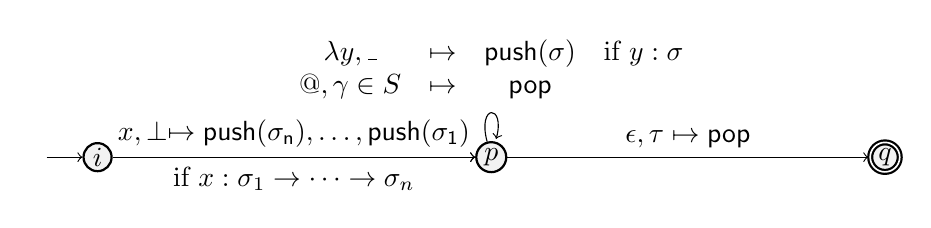
\begin{tikzpicture}[->, % makes the edges directed
%stealth’, % makes the arrow heads bold
node distance=5cm, % specifies the minimum distance between two nodes. Change if necessary.
every state/.style={thick, fill=gray!10, inner sep=1pt,minimum size=0pt}, % sets the properties for each ’state’ node
initial text=$ $,]
\node[state, initial] (q1) {$ i$};
\node[state,  right of=q1] (q2) {$ p$};
\node[state, accepting,right of=q2] (q3) {$ q$};
\draw 
(q1) edge[above] node{$
 x, \perp\mapsto \sf{push}(\sigma_n),\dots,\sf{push}(\sigma_1)$} (q2)
(q1) edge[below] node{$
 \text{if } x: \sigma_1\rightarrow\dots\rightarrow\sigma_n$} (q2)
(q2) edge[loop above] node{ $\begin{array}{cccc}
\lambda y, \_ &\mapsto& \sf{push}(\sigma) &   \text{if } y:\sigma\\
\text{@}, \gamma\in S &\mapsto &\sf{pop}&
\end{array}$} (q2)
(q2) edge[above] node{$
\epsilon, \tau \mapsto \sf{pop}
$} (q3);
\end{tikzpicture}
\end{center}
\end{itemize}
A word $w$ is accepted by $A_\tau$ if there is a run that reaches the end of $w$ in the accepting state $q$ with an empty stack. We write $(r, s)\xrightarrow{w} (r', s')$ if there is a run over the word $w$ which starts in the state $r\in Q$ and with a stack $s$ and ends up in the state $r'$ and with a stack $s'$.


By induction on the lenght of the word $w$, we can easily show that:
\begin{lemma}
For every word $w\in X.\{\text{@},\lambda x | x\in X \}^*$, we have that:
 $$(i, \perp)\xrightarrow{w} (p, \sigma_n\dots\sigma_1) \qquad\text{iff} \qquad 
w:\sigma_1\rightarrow\dots\rightarrow\sigma_n$$ 
\end{lemma}

A direct consequence of this lemma is that $A_\tau$ recognizes $W_\tau$. Another direct consequence is that the stack height of $A_\tau$ is bounded (let us say by a number $m$), since the set $S$ used to type the words is finite. Thus $A_\tau$ can be turned into an NFA $N_\tau$, by encoding the stack information in the states. More precisely, the states of $N_\tau$ are pairs $(r,s)$ where $r\in Q$ and $s$ is a stack of height at most $m$, the initial state is $(i,\perp)$ and there is a transition $(r,s)\xrightarrow{a}(r',s')$ where $a\in X_\lambda\cup\{\epsilon\}$ if there is a corresponding run in $A_\tau$. We show in the following that $N_\tau$ is counter-free. 

Let us start with some observations. In the automaton $A_\tau$, the effect of a word $w$ on a stack $s$, starting from the state $p$ is the following: it erases the first $n$ top level elements of $s$, and replaces them by a word $u$. The number $n$ and the word $u$ do not depend on the stack $s$ but only on the word $w$. This is exactly what the following lemma claims.

\begin{lemma}
For every word $w$ over ${X_\lambda}^*$, there is a natural number $n$ and a word $u\in S^*$ such that if $(p,s)\xrightarrow{w}(p,s')$ then $s$ and $s'$ can be decomposed as follows:
$$s=t.v,\qquad s'=t.u\qquad \text{ and }\qquad |v|=n.$$
\end{lemma}
The proof is an easy induction on the lenght of $w$. As a consequence we have that:
\begin{itemize}
\item If $(p,s_1)\xrightarrow{w}(p,s_2)\xrightarrow{w}(p,s_3)$ and $|s_2|>|s_1|$ then $|s_3|>|s_2|$.
\item If $(p,s_1)\xrightarrow{w}(p,s_2)\xrightarrow{w}(p,s_3)$ and $|s_2|<|s_1|$ then $|s_3|<|s_2|$.
\item If $(p,s_1)\xrightarrow{w}(p,s_2)\xrightarrow{w}(p,s_3)$ and $|s_2|=|s_1|$ then $s_3 =s_2$.
\end{itemize}

Let us show that $N_\tau$ is counter-free. Suppose by contradiction that there is a word $w$ and pairwise distinct stacks $s_1,\dots, s_n$ such that 
$(p,s_1)\xrightarrow{w}(p,s_2)\xrightarrow{w}\dots(p,s_n)\xrightarrow{w}(p,s_1)$. By the first two properties above, we have necessarily that $|s_1|=\dots=|s_n|$. Thus by the third property, we have that $s_1=\dots=s_n$, which concludes the proof.
\end{proof}



\subsection{Evaluation of linear $\lambda$-terms}

In this section we show that computing the normal form of $\linterm S X$ terms (that is well-typed linear $\lambda$-terms whose subterms have all types in $S$) is a derivable function:

 \begin{proposition}\label{prop:one-register} 
    For every typed set $X$ and every finite set $S$ of simple types, the function 
    \begin{align*}
        M \in  \linterm S X \qquad \mapsto \qquad \text{normal form of $M$} \in  \linterm S X
    \end{align*}
    is derivable.
\end{proposition}

The proof proceeds by induction on the set of types $S$. The main observation is that, if the evaluation of a redex of type $\sigma\rightarrow \tau$ creates new redexes, then their types are either $\sigma$ or $\tau$ (see Figure~\ref{}), they are in particular in $S\setminus\{\sigma\rightarrow\tau\}$. Thus, we only need to show that the function that evaluates all the redexes of a fixed type is derivable. As we only create stricty smaller redexes, we need to iterate this process only finitely many times, the bound being the size of $S$. 

  Since we have only finitely many typed variables, it is enough to show that the function that evaluates all the redexes of a fixed type $\sigma$ and a fixed variable $x$ is derivable. This will be our goal in the rest of this section.

\begin{theorem}\label{thm:evalOneType}
The function ${\sf{Eval}_{x,\sigma}}:\linterm S X \to\linterm S X$ which evaluates the redexes of type $\sigma$ and variable $x$ is derivable.
\end{theorem}


\subsubsection{Evaluation of thin $\lambda$-terms}

We start by showing that the evaluation of a restricted class of linear $\lambda$-terms, which we call thin, is an fo tree-to-tree function.   

\begin{definition}[Thin $\lambda$-terms]
A thin $\lambda$-terms is a term from $\rlambdalin$ in which a node is branching (ie a node having at least two sons which are not ports) if and only if it is a $\text{@}$ node, whose left son is a $\lambda x^\sigma$ node. We denote by $\rlambdathin$ the set of thin $\lambda$-terms.
\end{definition}

Since thin $\lambda$-terms branch only on redexes, the result of their evaluation is a word (that is, a term where every node has at most one son).  We will show that this word can actually be obtained by a pre-order traversal of the original $\lambda$-term. 
Since pre-order traversal is a basic fo tree-to-tree function, we can conclude that evaluation of thin $\lambda$-terms is a tree-to-tree function as well. 

\begin{center}
Picture 5
\end{center}

\begin{proposition}\label{prop:EvaluateThin}
There is an fo tree-to-tree function ${\sf{Eval}^{\sf{thin}}_{x^\sigma,\sigma\rightarrow\tau}}:\rlambda\to\rlambda$, whose restriction to $\rlambdathin$ evaluates the $x^\sigma$-redexes of type $\sigma\rightarrow\tau$.
\end{proposition}

\begin{proof}
Let $t$ be a thin $\lambda$-term and let $u$ be its normal form. As noticed before, $u$ has the shape of a word. Moreover, since $t$ is linear, the nodes of $u$ are exactly the nodes of $t$ which are not $x^\sigma$-redexes of type $\sigma\rightarrow\tau$, nor the nodes $x^\sigma$ they bind (ie. there is a label-preserving bijection $f$ between theses two sets of nodes).
We show that:
\noindent \begin{enumerate}
\item The order in which the inner nodes (ie. non ports) of $u$ appear is the tree order of $t$.
\item Let $n$ be a node of $u$ and $m$ be its corresponding node in $t$. The port $x$ of $u$ is the $i^{th}$ son of $n$ if and only if it the port $x$ of $t$ is the $i^{th}$ port of $m$.  
\end{enumerate} 

To establish the second claim, it is enough to show it for one step of $\beta$-reduction. But this last point is clear by a simple analysis of $\beta$-reduction, as far as we consider that the right son of the $\text{@}$ node of every redex is not a port. This is is guaranteed by the definition of thin $\lambda$-terms. 

To establish the first claim, let us consider two inner nodes $n, m$ of $t$ which are also nodes of $u$, and such that $n$ is smaller than $m$ is the tree order of $t$. We show that $n$ is a descendent of $m$ in $u$. There is two cases to consider:

\textbf{Case 1.} Either $n$ is a descendent of $m$ in $t$, in which case we can conclude easily since $\beta$-reduction preserves the descendent relation. Indeed, by a small analysis of $\beta$-reduction, one can notice that a reduction step may extend the descendent relation, but can never change (or break) the order of two comparable nodes in the original $\lambda$-term.    

\textbf{Case 2.} Otherwise, let us consider the lowest common ancestor $p$ of $m$ and $n$. We proceed by induction on the lenght of the path between $m$ and $p$. Notice first that since the only branching nodes of a thin term are $x^\sigma$-redexes, then $p$ is necessarily an $\text{@}$ node, whose left son $q$ is a $\lambda x^\sigma$ node. 
Notice first that $m$ is smaller than the free variable $r$ bound by $q$ w.r.t. the tree order. Indeed, if this was not the case, the free variable $r$ would not be bound by the node $q$, as illustrated by the following figure.
\begin{center}
Picture 6
\end{center}
We are then left with the following two situations:
\begin{center}
Picture 7
\end{center}    

Using these ingredients, let us construct now an fo tree-to-tree transduction which evaluates the $x^\sigma$-redexes of type $\sigma\rightarrow\tau$.
\begin{center}
Picture 8
\end{center}


    \begin{tabular}{ll}
    \pictureline
    {We start by tagging all the redexes of $t$ and their bound variables by $r$. This is an fo rational function, thus it can be performed by a derivable function. The result as a term in $\tmonad (\ranked{\mathcal{A}}+\ranked{\mathcal{A}^r})$, $\ranked{\mathcal{A}^r}$ being a copy of $\ranked{\mathcal{A}}$ where each element is tagged by $r$. Note that the nodes of $u$, the normal form of $t$, are the non-tagged node.}
    { \text{picture a}}
 \pictureline
    {We apply the pre-order traversal function. We get a term in $\tmonad \ranked{\Gamma}$ where $\ranked{\Gamma}:=\ranked{\mathcal{A}}+\ranked{\mathcal{A}^r}+\bullet+\bullet+\bullet$.}
    { \text{picture b}}
 \pictureline
    {Now we need to eliminate the tagged nodes. For that we start by adding the unary symbol $\#$ as a right son of each $\bullet$ node, getting a term in $\tmonad(\ranked{\Gamma+\#})$. This function is clearly derivable. }
    { \text{picture c}}
 \pictureline
    {We apply $\sf{block}^\uparrow$ to separate the symbol $\#$ from the others. We obtain a term in $\ranked{\tmonad(\tmonad \Gamma+\tmonad\#)}$}
    { \text{picture d}}
\pictureline
    {To each kind of blocks,  ($\ranked{\tmonad \Gamma}$ or $\ranked{\tmonad \#}$) we apply the functions $f: \ranked{\tmonad{\Gamma}} \to \ranked{\tmonad(\tmonad \Gamma+\tmonad\#)}$ and $g: \ranked{\tmonad{\#}} \to \ranked{\tmonad(\tmonad \Gamma+\tmonad\#)}$ which are both the identity function, except for the following elements:
    $$
    f(\bullet[\text{@}[\bullet,\bullet],p_1])=f(\bullet[\lambda x^\sigma\bullet],p_1])=f(\bullet[x^\sigma,p_1])=\bullet[p_1]$$
    
    For every n-ary element of $\ranked{\mathcal{A}}$, we have that:
 $$\begin{array}{c}
  f(\bullet[a[p_{i_1},\dots,p_{i_k}, \bullet, p_{i_{k+1}},\dots, p_{i_{n-1}}],p_{i_n}])\\
  =a[p_{i_1},\dots,p_{i_k}, p_{i_n}, p_{i_{k+1}},\dots, p_{i_{n-1}}]\\
f(\bullet[a[p_1,\dots,p_n]])=a[p_1,\dots,p_n]\\
g(\#[p_1])=p_1
\end{array}$$
After that, we apply a flattening, to get a term in $\ranked{\tmonad(\Gamma+\#)}$.
}
{ \text{picture e}}
\pictureline
{We have got the desired term, but not with the desired type. To obtain a term in $\ranked{\tmonad{\mathcal{A}}}$, we transform each tagged element of $\ranked{\mathcal{A}^r}$ into its untagged version, transform $\bullet_2$ into $\text{@}$, and $\bullet_0$ into $x^\sigma$. Finally, we erase the symbols $\#$ and $\bullet_1$.}{}
    \end{tabular}

 
\end{proof}

\subsubsection{$\beta$-reduction commutes with factorization} The second ingredient to show Thm.~\ref{thm:evalOneType} is to notice  that factorizing a term (in the sens of Def.~\ref{}), applying some $\beta$-reduction steps to the factors, then flattening, can be simulated by appliying  $\beta$-reduction steps directly to the original $\lambda$-term.

Let us state this property more formally. For that, we can generalise the lifting of functions to the lifting of relations as follows. 
Let $\Sigma$ be a ranked set. If $R\subseteq \ranked{\Sigma}\times\ranked{\Sigma}$ is an arity preseving relation (that is $\arity{u}=\arity{v}$ whenever $(u,v)\in R$), then $R$ can be lifted to $\tmonad R\subseteq \ranked{\tmonad \Sigma} \times \ranked{\tmonad \Sigma}$ in a natural way. 

Since $\beta$-reduction is an arity preserving relation  over linear $\lambda$-terms, its reflexive transitive closure $\beta^*$ is arity preserving as well.  We can lift then the later to $\tmonad \beta^*\subseteq \rlambdalin\times\rlambdalin$.
The following proposition is a direct consequence from the fact that $\beta$ is a congruence on terms.
  
\begin{proposition}\label{prop:betaCommutesWithFacto}
For every foctorization $f:\rlambda \to \tmonad \rlambda$, the following diagram commutes:
\begin{align*}
        \xymatrix{
     \rlambdalin \ar[d]_{\beta^*}\ar[r]^f& \tmonad \rlambdalin \ar[d]^{\tmonad\beta^*} \\
           \rlambdalin  &\ar[l]_{\sf{flat}} \tmonad \rlambdalin
        }
        \end{align*}
\end{proposition}



\subsubsection{Factorizing $\lambda$-terms into blocks of thin $\lambda$-terms}

\begin{definition}[Full redex]
Let $t$ be a linear $\lambda$-term. A full-redex is a set of nodes  containing an $x^\sigma$-redex of type $\sigma\rightarrow\tau$, the node $x^\sigma$ it binds, together with the set of nodes between the binder of the redex and its bound variable.  
\end{definition}
\begin{center}
Picture 9
\end{center}


\begin{proposition}\label{prop:FactoIntoThin}
There is an fo tree-to-tree factorisation $f:\rlambda \to \tmonad\rlambda$ such that for every $t\in\rlambdalin$
\begin{itemize}
\item any full redex of $t$ is entirely contained in one of the factors of $f(t)$;
\item the factors of $f(t)$ are thin $\lambda$-terms.
\end{itemize}
\end{proposition}

\begin{proof}
Let us constract an fo derivable factorization satisfying the two conditions of the statement.  

 \begin{tabular}{ll}
    \pictureline{We start by tagging all the redexes and their bound variables by $r$. The result as a term in $\tmonad (\ranked{\mathcal{A}}+\ranked{\mathcal{A}^r})$, $\ranked{\mathcal{A}^r}$ being a copy of $\ranked{\mathcal{A}}$ where each element is tagged by $r$. We set $\ranked{\mathcal{A}'}:= \ranked{\mathcal{A}+\mathcal{A}^r}$}{}
    \pictureline{We add the unary symbol $\#$ as a parent of each tagged symbol $\lambda x^\sigma$, then we apply a $\sf{block}^\uparrow:\ranked{\tmonad(\mathcal{A}'+\#)}\to \ranked{\tmonad(\tmonad(\mathcal{A}')+\tmonad\#})$. Doing so, each block $\ranked{\tmonad(\mathcal{A}')}$ contains at most one tagged binder $\lambda x^\sigma$ and the (tagged) variable $x^\sigma$ it binds.}{}
	\pictureline{To each block $\ranked{\tmonad(\mathcal{A}')}$, we apply the fo-rational function $f:\ranked{\tmonad{\mathcal{A}'}}\to \ranked{\tmonad(\mathcal{A}'_++\mathcal{A}'_-)}$, which adds $+$ to the nodes having as descendent a tagged node $x^\sigma$, and adds $-$ to the others.  }{}
   \pictureline{To each block $\ranked{\tmonad(\mathcal{A}'_++\mathcal{A}'_-)}$, we apply $\sf{block}^\uparrow: \ranked{\tmonad(\mathcal{A}'_++\mathcal{A}'_-)}\to \ranked{\tmonad(\tmonad(\mathcal{A}'_+)+\tmonad(\mathcal{A}'_-))}$. By linearity, each $\ranked{\tmonad(\mathcal{A}'_+)}$ block is a thin $\lambda$-term containing the path from a binder to its free variable.
    }{}
    \pictureline{Now, we erase the blocks $\ranked{\tmonad{\#}}$ and apply flat. We get a term in $\ranked{\tmonad(\tmonad(\mathcal{A}'_+)+\tmonad(\mathcal{A}'_-))}$.}{}
    \pictureline{We apply $\sf{block}^\uparrow:  \ranked{\tmonad(\tmonad(\mathcal{A}'_+)+\tmonad(\mathcal{A}'_-))}\to \ranked{\tmonad(\tmonad\tmonad(\mathcal{A}'_+)+\tmonad\tmonad(\mathcal{A}'_-))}$, then flat each block $\ranked{\tmonad\tmonad(\mathcal{A}'_+)}$ and $\ranked{\tmonad\tmonad(\mathcal{A}'_-)}$. We obtain a term in $\ranked{\tmonad(\tmonad(\mathcal{A}'_+)+\mathcal{A}'_-)}$, where each block $\ranked{\tmonad(\mathcal{A}'_+)}$ is a thin $\lambda$-term. Moreover, every redex is contained in a $\ranked{\tmonad(\mathcal{A}'_+)}$ block, except for the redexes whose binders are the roots of the  $\ranked{\tmonad(\mathcal{A}'_+)}$ blocks. To conclude, one only needs to add the $\text{@}$ above each such binder to its correponding block. }{}
    \pictureline{For that, we add the unary symbol $\#$ as a right son of each tagged $\text{@}$ symbol of $\mathcal{A}'_-$. We obtain a term in $\ranked{\tmonad(\tmonad(\mathcal{A}'_+)+\mathcal{A}'_-+\#)}$. Then we apply $\sf{block}^\uparrow:\ranked{\tmonad(\tmonad(\mathcal{A}'_+)+\mathcal{A}'_-+\#)}\to \ranked{\tmonad(\tmonad(\tmonad(\mathcal{A}'_+)+\mathcal{A}'_-)+\tmonad{\#})}$}{}
    \pictureline{We eliminate the blocks $\ranked{\tmonad{\#}}$ and apply flat, thus getting a term in $\ranked{\tmonad(\tmonad(\mathcal{A}'_+)+\mathcal{A}'_-)}$. We reapply block to seperate the blocks $\ranked{\tmonad(\mathcal{A}'_-})$ from the others, apply some flatening and eliminate all the taggs ($r$, +, -), in orther to get a term in $\ranked{\tmonad(\tmonad(\mathcal{A}))}$.}{}
    
    
   \end{tabular}
   
\end{proof}

\subsubsection{Gathering all the pieces.}
Theorem~\ref{thm:evalOneType} follows easily from Propositions~\ref{prop:EvaluateThin},\ref{prop:betaCommutesWithFacto} and \ref{prop:FactoIntoThin}.

\begin{proof}[Proof of Theorem.~\ref{thm:evalOneType}]
Let us show that the evaluation of all  $x^\sigma$-redexes of type $\sigma\rightarrow\tau$ is derivable. We start by applying to our $\lambda$-term the factorisation $f$ from Prop.~\ref{prop:FactoIntoThin}. As the factors are thin $\lambda$-terms, we can evaluate them by lifting the function from Prop.~\ref{prop:EvaluateThin}. We apply a flat to obtain again a $\lambda$-term. The later is a $\beta^*$-redex of the original $\lambda$-term by Prop.~\ref{prop:betaCommutesWithFacto}. Moreover, since every full-redex of the original $\lambda$-term was in one of the factors, all the $x^\sigma$-redexes has been reduced, which concludes the proof. 
\end{proof}
\section{Decomposing the prime function unfold}
\label{ap:matrix-power}
\newcommand{\treeunfold}{\mathrm{unfold}}

Among our prime functions, the less satisfactory one is certainly the unfloding function. In this section, we will decompose it into a collection of functions containing no form of iteration. 



\subsection{New prime functions replacing the unfolding}\label{sec:functions-decomposing-unfolding}

The prime functions which are intended to replace the unfolding function use a new datatype constructor called \emph{shallow terms}. it is defined as follows.  

\paragraph*{Shallow terms.} Let $\rSigma$ and $\rGamma$ be two ranked sets. An element of the shallow terms datatype denoted $\shallowterm \rSigma \rGamma$, is an expression of the form $a\tensorpair{b_1,\dots,b_n}$ where $a$ is an $n$-ary element of $\rSigma$ and $b_1,\dots, b_n$ are elements of $\rGamma$. We draw shallow terms like this:
\mypic{54}
Clearly, a shallow term is just a particular case of terms.

\paragraph*{New prime functions.} Let us present now the prime functions which will replace the unfolding function. Prime functions of Figure~\ref{fig:prime-for-shallow-terms} are some basic functions for the new shallow term datatype. Figure~\ref{fig:additional-distrib-prime} contains some new ditributivity laws and Figure~\ref{fig:additional-prime-for-fold} contains some additional laws for the fold datatype. Prime functions of Figure~\ref{fig:weak-unfolding} are weak versions of the unfolding function, containing no form of iteration. 

\begin{figure}
\fbox{
\begin{minipage}{1\linewidth}
\begin{itemize}
\item \textbf{Unit.}
$$
\begin{array}{c}
 \ranked{\Sigma} \ \ \ranked{\leftrightarrow} \ \    \ranked{ \Sigma \cdot 1}\\[5pt]
        {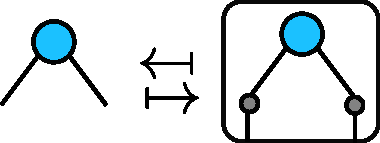
\includegraphics[scale=.4]{pictures/sigma-dot-1}} 
\end{array}
$$
\item \textbf{Associativity.}
$$
\begin{array}{c}
 \ranked{(\Sigma \cdot \Gamma)\cdot \Delta } \ \ \ranked{\to} \ \    \ranked{ \Sigma \cdot (\Gamma \cdot \Delta)}\\[5pt]
        {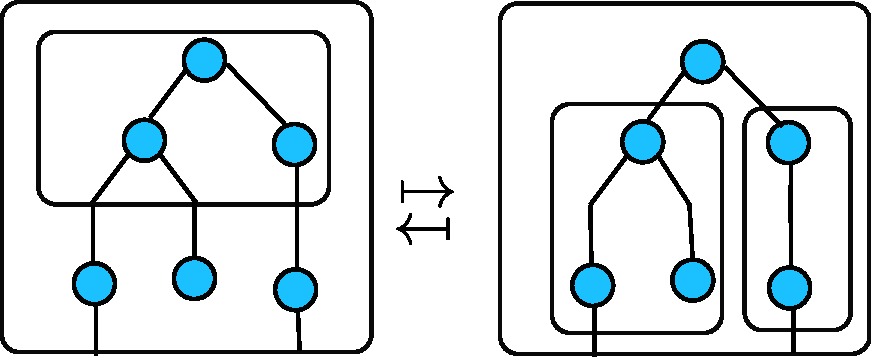
\includegraphics[scale=.4]{pictures/associativity-shallow}} 
\end{array}
$$
\item \textbf{Terms as shallow terms.}
$$
\begin{array}{c}
 \ranked {1 + \shallowterm \Sigma {\tmonad \Sigma}\ \ \to \ \  \tmonad \Sigma}\\[5pt]
        {
        \begin{tabular}{l}
            Every term is either just a port,\\ or has a root and child subterms.    
        \end{tabular}    
        }
\end{array}
$$
\item \textbf{Tensors as shallow terms.}
$$
\begin{array}{c}
\ranked {\Sigma^n \ \ \leftrightarrow \ \ \shallowterm n \Sigma}\\[5pt]
        {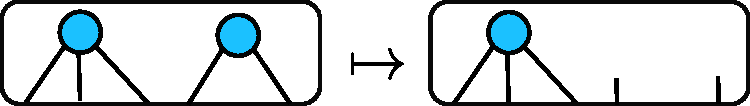
\includegraphics[scale=.4]{pictures/tensor-projection-1}}
\end{array}
$$
\end{itemize}
\end{minipage}
}
\caption{Prime functions for shallow terms.}\label{fig:prime-for-shallow-terms}
\end{figure}

\begin{figure}
\fbox{
\begin{minipage}{1\linewidth}
\begin{itemize}
\item \textbf{Unit.}
$$
\begin{array}{c}
 \ranked{\Sigma \ \ \to \ \ \reduce k \Sigma^k}\\[5pt]
        {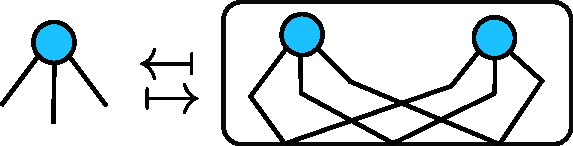
\includegraphics[scale=.4]{pictures/tensor-injection}}
\end{array}
$$
\item \textbf{Increase fold.}
$$
\begin{array}{c}
 \ranked{\reduce k \Sigma \ \ \to \ \ \reduce {k+1}\Sigma}\\[5pt]
        {
\includegraphics[scale=.4]{pictures/add-fold}}	
\end{array}$$
\item \textbf{Decrease fold.}
$$
\begin{array}{c}
 \ranked{\reduce {k+1} \Sigma \ \ \to \ \ \reduce {k}\Sigma+\bot}\\[5pt]
        {
\includegraphics[scale=.4]{pictures/reduce-fold}}	 
\end{array}$$
\item \textbf{projection of copairs.}
$$
\begin{array}{c}
   \ranked{\Sigma\product \Sigma \ \ \to \ \ \reduce 1 \Sigma}\\[5pt]
        {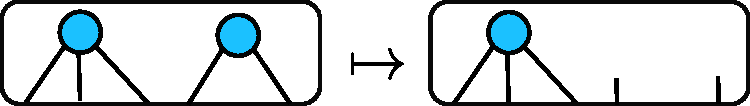
\includegraphics[scale=.4]{pictures/tensor-projection-1}}	
\end{array}$$
\end{itemize}
\end{minipage}
}
\caption{Additional prime functions for folds.}\label{fig:additional-prime-for-fold}
\end{figure}

\begin{figure}
\fbox{
\begin{minipage}{1\linewidth}
\begin{itemize}
\item \textbf{Folds over pairs.}
$$
\begin{array}{rll}
  \ranked{\reduce k (\Sigma_1 + \Sigma_2)}& \ranked{\to} & \ranked{\reduce k \Sigma_1 + \reduce k \Sigma_2}\\
         (a,i)/f & \mapsto & ((a/f),i)
\end{array}
$$
\item \textbf{Shallow terms over pairs.}
$$
\begin{array}{rll}
  {\shallowterm {(\Sigma_1 + \Sigma_2)} \Gamma} & \ranked{\to} & \ranked{(\shallowterm {\Sigma_1} \Gamma) + (\shallowterm {\Sigma_2} \Gamma)}\\
        (a,i)\tensorpair{t_1,\dots,t_n} &\mapsto& (a\tensorpair{t_1,\dots,t_n},i)
\end{array}
$$
\item \textbf{Shallow terms over copairs.}
$$
\begin{array}{c}
  \ranked{{\shallowterm {(\Sigma_1 \product \Sigma_2)} \Gamma}
   \ \  \to \ \ {(\shallowterm {\Sigma_1} \Gamma) \product (\shallowterm {\Sigma_2} \Gamma)}}\\[5pt]
        {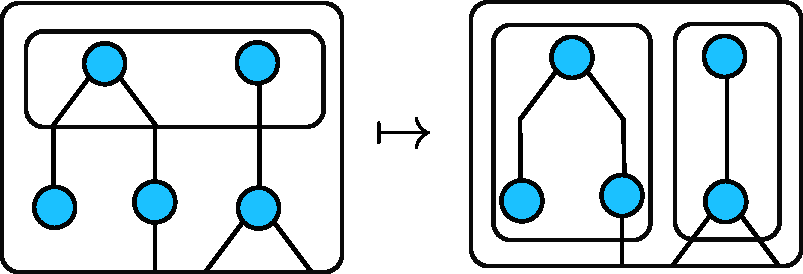
\includegraphics[scale=.4]{pictures/tensor-shallow-distrib}}
        \end{array}
$$
\item \textbf{Folds over copairs.}
$$
\begin{array}{c}
\ranked{(\reduce k \Sigma_1) \product (\reduce k {\Sigma_2}) \ \ \to \ \reduce k (\Sigma_1 \product \Sigma_2)}\\[5pt]
        {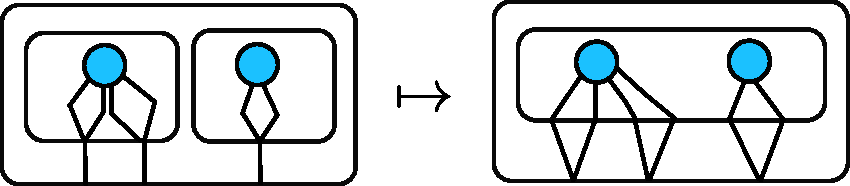
\includegraphics[scale=.4]{pictures/tensor-fold-distrib-2}}  
\end{array}
$$
\item \textbf{Folds over copairs (bis).}
$$
\begin{array}{c}
    \ranked{\reduce k (\Sigma_1 \product \Sigma_2) \ \ \to \ \ \reduce k ((\reduce k {\Sigma_1})\product (\reduce k \Sigma_2))}\\[5pt]
        {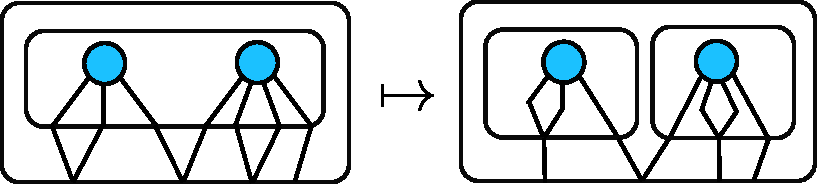
\includegraphics[scale=.4]{pictures/tensor-fold-distrib-1}}   
\end{array}
$$
\item \textbf{Shallow terms over folds.}
$$
\begin{array}{c}
 \ranked{\shallowterm \Sigma {\reduce k \Gamma}\ \ \to \ \ \reduce k (\shallowterm \Sigma {\Gamma})}\\[5pt]
 {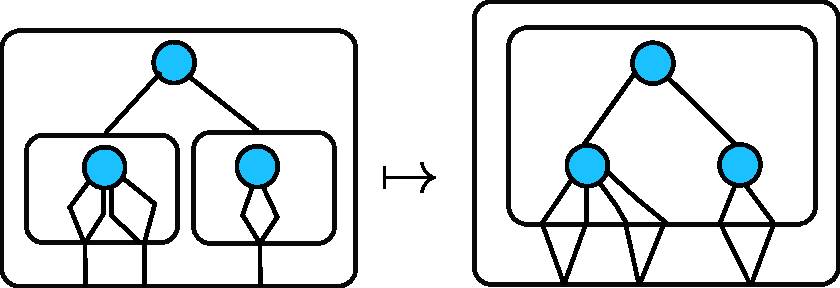
\includegraphics[scale=.4]{pictures/shallow-fold-distrib}} 
\end{array}
$$
\item \textbf{Folds over shallow terms.} 
$$
\begin{array}{c}
 \ranked{\reduce k \Sigma\cdot \Gamma\ \ \to \ \ (\reduce k \Sigma) \cdot \mati k \Gamma}\\[5pt]
 {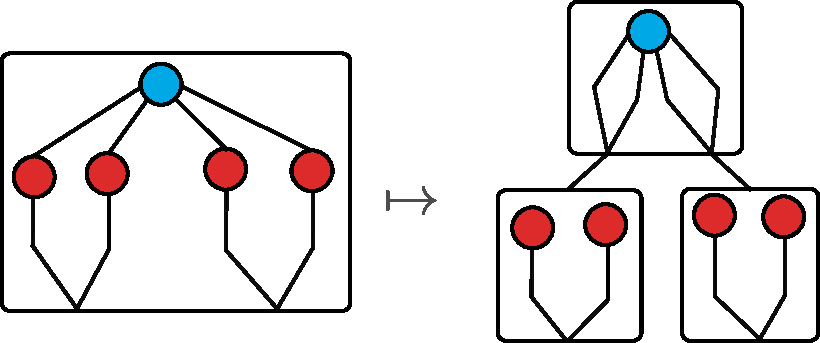
\includegraphics[scale=.4]{pictures/last-prime-function}} 
\end{array}
$$
$\rGamma$ is a set of unary elements.
\end{itemize}
\end{minipage}
}
\caption{Additional distributivity prime functions.} \label{fig:additional-distrib-prime}
\end{figure}

\begin{figure}
\fbox{
\begin{minipage}{1\linewidth}
\begin{itemize}
\item \textbf{Untwist.}
$$
\begin{array}{c}
\ranked{\tmonad {\reduce 1\Sigma} \ \  \to \ \ \reduce 1 \tmonad \Sigma}\\[5pt]
         {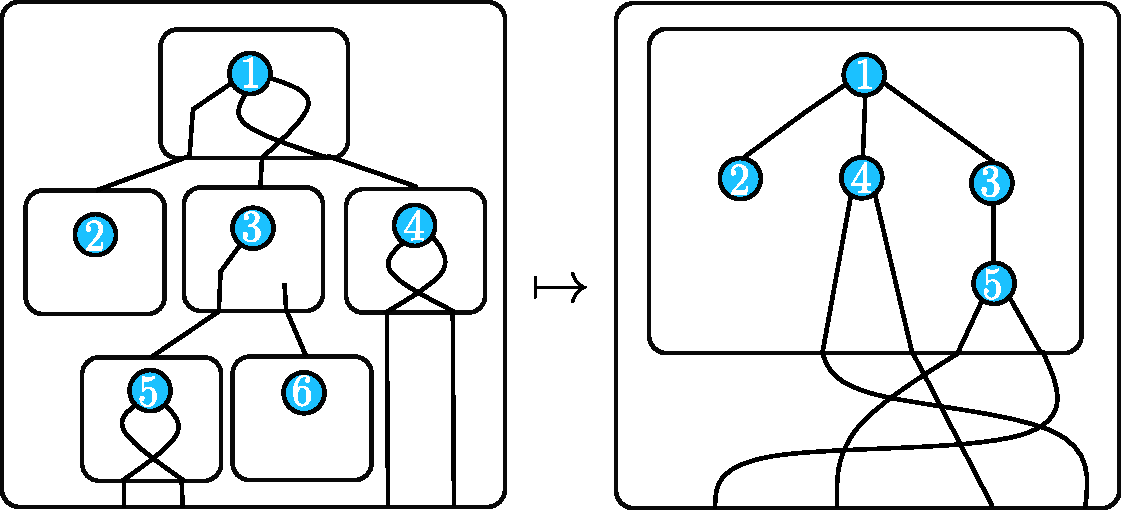
\includegraphics[scale=.4]{pictures/unfold-1}}
\end{array}
$$
\item \textbf{External fold.}
$$
\begin{array}{c}
\ranked{\tmonad {\reduce k\Sigma} \ \  \to \ \ \reduce k \tmonad \reduce k\Sigma}\\[5pt]
         {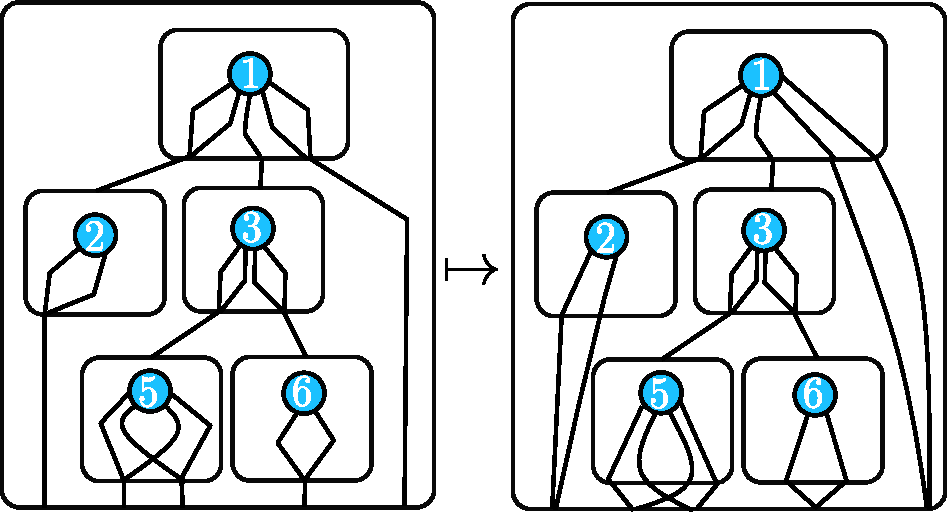
\includegraphics[scale=.43]{pictures/external-unfold-1}}
\end{array}
$$
\item \textbf{Matching.}
$$
\begin{array}{c}
\ranked{\shallowterm {\reduce k \Sigma}{\Gamma^k} \ \ \to \ \ \reduce 1(\shallowterm \Sigma \Gamma)}\\[5pt]
\includegraphics[scale=.3]{pictures/shallow-unfold}
\end{array}
$$
\end{itemize}
\end{minipage}
}
\caption{Weak forms of unfolding.}\label{fig:weak-unfolding}
\end{figure}


The main result of this section is that the unfolding can be replaced by the more atomic functions of Figures~\ref{fig:prime-for-shallow-terms}, \ref{fig:additional-distrib-prime}, \ref{fig:additional-prime-for-fold} and ~\ref{fig:weak-unfolding}, in  presence of the other prime functions presented in Section~\ref{sec:derivable-functions}, as stated in the following theorem
 
\begin{theorem}\label{thm:decompose-unfolding}
The unfolding function can be derived using the functions of Figures~\ref{fig:prime-for-shallow-terms}, \ref{fig:additional-distrib-prime}, \ref{fig:additional-prime-for-fold}, ~\ref{fig:weak-unfolding}, and the prime functions of Section~\ref{sec:derivable-functions}.
\end{theorem}

%\subsection{Decomposing the unfolding function}\label{sec:proof-decompose-unfold}


Our proof strategy is to show that term unfolding can be derived for certain homogeneous (see below) monotone inputs, and then to show that every input can be decomposed into simpler inputs in a homogeneous way. The notion of homogeneous inputs, and the result about  decomposing of arbitrary inputs into homogeneous inputs, are presented in Section~\ref{sec:factfor}. Next, in Section~\ref{sec:homo-unfold}, we show how term unfolding can be done for homogeneous inputs. Finally, in Section~\ref{sec:monotone-unfold-proof} we prove Theorem~\ref{thm:decompose-unfolding} by combining  the results of Sections~\ref{sec:factfor} and~\ref{sec:homo-unfold}.

\subsection{Factorisation forests}
\label{sec:factfor}
This section is devoted to stating and proving a tree version of the Factorisation Forest Theorem of Imre Simon.  Our result differs from the original Factorisation Forest Theorem in the following ways: (a) we consider trees instead of strings; (b) we use aperiodic finite monoids instead of arbitrary finite monoids; and (c) the factorisation in the conclusion of the theorem can be computed by a derivable function.  A tree generalisation of the Factorisation Forest Theorem was already proved by Colcombet~\cite[Theorem 1 and Section 3.3]{colcombetCombinatorialTheoremTrees2007}, but Colcombet's result is proved for monadic second-order logic, and therefore it does not satisfy condition (c). 



\paragraph{Factorisation forests} The idea behind factorisation forests is to split a term into a nested factorisation, which is a term of terms of terms, and so on up to a certain depth.  
Define a \emph{nested factorisation} of depth $k \in \set{1,2,\ldots}$ over alphabet $\rSigma$ to be an element of $\tmonadn k \rSigma$ which is defined by
\begin{align*}
\tmonadn 0 \rSigma = \rSigma  \quad \text{and} \quad \tmonadn {k+1}\rSigma = \tmonad \tmonadn k \rSigma.
\end{align*}
Nested factorisations can be flattened to terms by using an  operation $\flatn k : \tmonadn k \rSigma \rto \tmonad \rSigma $ defined by 
\begin{align*}
     \flatn 1 = \text{\ranked{identity}} \quad \text{and} \quad  \flatn {k+1} \eqdef \flatt  \circ \tmonad \redpar { \flatn k}.
\end{align*}
An equivalent definition of $\flatn {k+1}$ would be $\flatn k \circ \tmonadn {k-1} \flatt$, the equivalence of these definitions corresponds to the fact that $\tmonad$ is a monad.


\paragraph{Branches and subbranches}
Define a \emph{branch} in a ranked set to be an element  of the ranked set together with a distinguished port. 
We draw branches like  this:
\mypic{82}
We write $\branches \rSigma$ for the (unranked) set of branches over a ranked set $\rSigma$. \label{page:branches}
For a term, we classify its edges as internal (linking a non-port node with a non-port child) and external (linking a non-port node with a child port). Each edge in a term $t \in \tmonad \rSigma$ corresponds to a branch over $\rSigma$, namely the branch which leads to the edge. Any branch obtained this way is called a \emph{subbranch} of $t$. Here is a picture of subbranches in the case of a term of terms:
\mypic{80} 

\newcommand{\hb}[2]{#2^{(#1)}}
Branches in  terms  form a monoid. Using the monoid structure of branches in terms, we can extend any function  $h : \branches \rSigma \to M$, with $M$ a monoid, to a  monoid homomorphism
\begin{align*}
\hb n h : \branches \tmonadn n \rSigma \to M
\end{align*}
which maps a branch of a term to the product -- in the monoid $M$ -- of all of its subbranches (after flattening).  A more formal definition is that $\hb 0 h$ is the same as $h$, while  $\hb {n+1} h$  is the unique monoid homomorphism  which makes the following diagram commute
\begin{align*}
\xymatrix{
    \branches \tmonadn n \rSigma \ar[dr]^{\hb n h} \ar[d]_{\branches \unit}\\
    \ar[r]_{\hb {n+1}  h}\branches \tmonadn {n+1} \rSigma & M
}
\end{align*}


The idea behind factorisation forests, as expressed in Definition~\ref{def:hom-for} below, is to factorise a term into a term of terms of terms (etc.) so that the depth of nesting is bounded, and at each level all branches behave regularly with respect to some monoid homomorphism. 

\begin{definition}[Homogeneous factorisations]\label{def:hom-for}
    Let $h : \branches \rSigma \to M$ be a function into a monoid $M$. 
    \begin{itemize}
\item     We say that a factorisation $t \in \tmonad \tmonad \rSigma$ is \emph{homogeneous with respect to $h$} if it either:
\begin{enumerate}
    \item \label{it:factfor-shallow} it is a shallow term (which means that all internal edges originate from the root); or 
    \item \label{it:factfor-allsame} all internal subbranches of $t$ have the same value under $\hb 1 h$; or
    \item \label{it:factfor-ab} if $a,b \in M$ appear as values -- under $\hb 1 h$ -- of internal branches in $t$, then $ab=a$. 
\end{enumerate}
\item We say that a nested factorisation  $t \in \tmonadn n \rSigma$ is \emph{hereditarily homogeneous with respect to $h$} if either $n=1$ and $t$ is the unit of a letter, or $n \ge 2$ and both:
\begin{enumerate}
    \item  it is homogeneous with respect to $\hb {n-1} h$; and 
    \item every node has a label in $\tmonadn {n-1} \rSigma$ that is hereditarily homogeneous with respect to $h$.
\end{enumerate}
    \end{itemize}
\end{definition}


Recall that a finite monoid is aperiodic if it has only trivial subgroups. An equivalent definition is that every element $m$ of the monoid satisfies 
\begin{align*}
  \exists n \in \set{1,2,\ldots}\   m^n = m^{n+1}.
\end{align*} 
A famous theorem of Sch\"utzenberger, McNaughton and Papert, see~\cite[Theorem VI.1.1]{straubingFiniteAutomataFormal1994} says that the languages  of words recognised by homomorphisms into finite aperiodic monoids are exactly  those that can be defined in first-order logic. This is the reason why  we consider aperiodic monoids.

\begin{example}\label{ex:partial-monoton-functions}
   Let $k \in \set{1,\ldots}$ and  consider the monoid of partial functions 
    \begin{align*}
    \set{1,\ldots,k} \to \set{1,\ldots,k}.
    \end{align*}
    This monoid is not aperiodic, because it contains the  group of all permutations of $\set{1,\ldots,k}$. Consider now the restriction of this monoid to partial functions which are monotone (this is a monoid, because such functions are closed under composition). This monoid is aperiodic, because if $f$ is a partial function, then for  every $i \in \set{1,2,\ldots,k}$ the sequence
    \begin{align*}
    f^1(k),f^2(k),f^3(k),\ldots
    \end{align*}
    reaches a fixpoint (or becomes undefined) in at most $k$ steps.
\end{example}
We are now ready to state our version of the Factorisation Forest Theorem. 
\begin{theorem}[Factorisation Forest Theorem]\label{thm:factfor}
    Let $\rSigma$ be a  ranked set and let $h : \branches  \rSigma \to M$ be a function into a finite aperiodic monoid $M$. There is some $n \in \set{1,2,\ldots}$ and a  function
    \begin{align*}
        \ranked {f : \tmonad \rSigma \to \tmonad^n \rSigma}  
    \end{align*}
such that $\flatn n \circ \ranked f$ is the identity on $\tmonad \rSigma$, and  all outputs of  $\ranked f$ are hereditarily homogeneous with respect to $h$. Furthermore, if $\rSigma$ is finite\footnote{This finiteness assumption could be relaxed by saying that $\rSigma$ is possibly infinite but the function $h$ is derivable, in the sense that a derivable function can decorate the ports of an element in $\rSigma$ by their values under $M$.} then $\ranked f$ is derivable. 
\end{theorem}



\newcommand{\hint}{\bar h}
\newcommand{\hintplus}{\bar h^+}
\newcommand{\branchesplus}{\mathsf B^+}


% Later in this section, we also give a sufficient condition which ensures that $\ranked f$ as in the theorem is derivable, by analysing in more detail the proof the theorem. 
In the proof below, the constructions  are designed so that they can be formalised using derivable functions, however we leave the details of  the ``Furthermore'' part to the reader. 

Define a \emph{good set} to be any subset  $\ranked X \subseteq  \tmonad \rSigma$ which admits a function 
\begin{align*}
    \ranked {f : \tmonad \rSigma \to \tmonad^n \rSigma}   \qquad \text{for some $n \in \set{1,2,\ldots}$}
\end{align*}
such that $\flatn n \circ \ranked f$ is the identity on $\tmonad \rSigma$, and    $\ranked f$ restricted to $\ranked X$ produces only hereditarily homogeneous outputs. Our goal is to show that the entire set $\tmonad \rSigma$ is good. To prove this, we use a more refined result, stated below, which has a parameter  that can be used for  induction.  We say that a term $t \in \tmonad \rSigma$ uses $A \subseteq M$ for  internal subbranches if all  internal subbranch have image under $\hb 1 h$ that belongs to $A$. 

\begin{lemma}\label{lem:fact-ind}
    Let $\rSigma$ be a  ranked set and let $h : \branches \tmonad \rSigma \to M$ be a monoid homomorphism into a finite aperiodic monoid $M$. For every $A \subseteq M$, the  terms that use $A$ for inner subbranches  is good.
    \end{lemma}

\newcommand{\subgen}[1]{\langle #1 \rangle}
Theorem~\ref{thm:factfor} follows immediately from the  lemma, by taking $A$ to be the entire monoid. The rest of Section~\ref{sec:factfor} is therefore devoted to proving the lemma. The proof is by induction on  two parameters: (a) the size of $A$; and (b) 
the size of the semigroup $\subgen A \subseteq M$ that is  generated by $A$.
 These parameters are  ordered lexicographically, with the size of the semigroup being more important.

The induction base is when $A$ contains only one element $a$ of the monoid. If a term uses $\set a$ for  internal subbranches, then applying $\tmonad \unit$ leads to a factorisation that is  homogeneous according to item~\ref{it:factfor-allsame} of Definition~\ref{def:hom-for}, which is also hereditarily homogeneous because all nodes are labelled by units. This completes the proof of the induction base.

In the proof of the induction step, we consider two cases.
\begin{itemize}
    \item The first case is  when  every $a \in A$ satisfies 
    \begin{align*}
       \subgen{\set{ b a :  b \in \subgen A}} = \subgen A
  \end{align*}
  This means that every for every $a \in A$, the function $b \mapsto ba$ is a permutation of $\subgen A$. Since the monoid is aperiodic, this permutation must necessarily be the identity.  Therefore, we have $ab=a$ for every $a,b \in \subgen A$. This means that if all a term uses $A$ for  internal subbranches, then applying $\tmonad \unit$  gives a factorisation which is hereditarily homogeneous according to item~\ref{it:factfor-ab} of Definition~\ref{def:hom-for}. 
    \item If the previous item does not hold, then there is some $a \in A$ such that 
    \begin{align*}
         \subgen{\set{ b a :  b \in \subgen A}}
    \end{align*}
    is a proper subsemigroup of $\subgen A$.  Fix some such $a$.  Define a \emph{sensitive edge} in a term  $t \in \tmonad \rSigma$ to be any internal edge where the corresponding subbranch has value $a$ under  $\hb 1 h$. Call an internal edge \emph{post-sensitive} if it is not sensitive, but its parent edge is. Here is a picture:
    \begin{center}
\includegraphics[scale=.27, page=8]{pics}
\end{center}
    Define the \emph{split} of a term to be the factorisation which  cuts along post-sensitive  edges, as shown in the following picture:
    \begin{center}
\includegraphics[scale=.29, page=88]{pics}
\end{center}
    We only consider splits for terms which use $A$ for internal subbranches. Roughly speaking,  we will show that all factors in the split are good, and the split itself is good.  Combining these two observations, we will see that all terms 

    We begin by looking at the factors in the split (of a term where $A$ is used for internal subbranches). Here is a picture of such a factor:
    \mypic{89}
        If we follow a  branch in an factor of the split, from root to port, we first  have a sequence of non-sensitive  edges from the original term, followed by a sequence of sensitive edges. Group the non-sensitive edges together, and group the sensitive edges together, resulting in a shallow term from $\shallowterm{\tmonad \rSigma}{\tmonad \rSigma}$, which is illustrated in the following picture:
     \begin{center}
\includegraphics[scale=.3, page=90]{pics}
\end{center}
        In the resulting shallow term,  the root is labelled by a term without sensitive edges (i.e.~it is a term which uses $A - \set a$ for internal subbranches), while the children are labelled by terms where all edges are sensitive (i.e.~they are terms which use $\set a$ for internal subbranches). We can apply the induction in both cases, and combine the resulting nested factorisations using a shallow term, as in item~\ref{it:factfor-shallow} of Definition~\ref{def:hom-for}.

        Having established that the factors of the split are good, we turn to the split itself. By construction, every subbranch of the split is mapped by $\hb 1 h$ to the smaller semigroup 
        \begin{align*}
            \subgen{\set{ b a :  b \in \subgen A}},
       \end{align*}
       We can  view the  split as a term over alphabet $\rGamma = \tmonad \rSigma$.  Since all  internal subbranches of the split are in the smaller subsemigroup, we can apply the induction assumption of the lemma (with $\rGamma$ and $\hb 1 h$), showing that the split is good. More formally, the set 
       \begin{align*}
       \set{\text{split of $t$} : t \in \tmonad  \rGamma \text{ uses $A$ for internal subbranches}}
       \end{align*}
       is good. To show now that original set of terms $t$ that use $A$ for  internal branches is good, we first apply the split, then compute the nested factorisation for the split, and finally we compute the nested factorisations for the factors of the split (the letters from $\rGamma$.). 
\end{itemize}


% We now give a proof sketch of the ``Furthermore'' part in the theorem, which says that if $\rSigma$ is finite, then
% \begin{align*}
%     \ranked {f : \tmonad \rSigma \to \tmonad^k \rSigma}  
% \end{align*}
% in the conclusion of the theorem not only exists, but it is derivable. In the proof sketch, we will appeal to the power of first-order tree relabellings from Section~\ref{sec:fo-translation}. To use tree relabellings, define \emph{pseudo-flattening} to be the  function 
% \begin{align*}
% \ranked{\mathrm{pseudoflat}} : \tmonad \tmonad \rSigma \rto \tmonad\redpar{\rSigma \redplus \redset{\overbrace{\text{open},\text{close}}^{\text{arity 2}}}}
% \end{align*}
% which adds an ``open'' whenever a new factor starts and adds a ``close'' letter whenever a factor ends, as depicted in the following picture:
% \mypic{91}
% Pseudo-flattening can be lifted in a natural way to nested factorisations 
% \begin{align*}
%     \ranked{\mathrm{pseudoflat}_n : \tmonadn {n+1} \rSigma \rto \tmonad \Sigma_n} \qquad \text{where }\ranked{\Sigma_n} \eqdef \redpar{\rSigma \redplus \redset{\overbrace{{\text{open}_i,\text{close}_i }}^{\text{arity 2}: i \in \set{1,\ldots,n}}}}
% \end{align*}
% Call a function $\ranked f$  \emph{pseudo-derivable} if there  is a derivable $\ranked g$ which makes the following diagram commute
%     \begin{align*}
%     \ranked{
%         \xymatrix{
%             \tmonad \rSigma \ar[r]^f \ar[d]_{\mathrm{pseudoflat}}& \tmonadn n \rSigma \ar[d]^{\mathrm{pseudoflat_n}} \\
%             \tmonad \rSigma_1 \ar[r]_g & \tmonad \rSigma_n 
%         }
%     }
%     \end{align*}
    
% \begin{lemma}\label{lem:pseudo-der}
%     A function $\ranked f$ is derivable if and only if it is pseudo-derivable.    
% \end{lemma}
% \begin{proof}
%     (Sketch.) Pseudo-flattening and its nested extensions are  easily seen to be derivable, and the same is true for their (one-sided) inverses.  
% \end{proof}
 
% The advantage of  pseudo-flattening  is that it allows use to work with first-order tree relabellings, which are much easier to work with. By an analysing the proof of Lemma~\ref{lem:fact-ind}, one can show that if $\rSigma$ is finite, then  the function $\ranked f$ is pseudo-derivable. This is because the basic operations in the proof of the lemma, such as ``find the first sensitive edge'' can easily be formalised in first-order logic, which in turn can be turned into derivable functions by virtue of Proposition~\ref{prop:forat}. 
\subsection{Term unfolding for homogeneous inputs}
\label{sec:homo-unfold}
For a monotone function 
\begin{align*}
\alpha: \set{1,\ldots,k} \to \set{1,\ldots,k}
\end{align*}
we say that a term $ t \in \tmonad \mati k \rSigma$ is $\alpha$-homogeneous if all internal branches have twist $\alpha$. This section is devoted to proving the following lemma. 

\begin{lemma}\label{lem:homo-twist}
    Let $k \in \set{1,2,\ldots}$ and let $\alpha : \set{1,\ldots,k} \to \set{1,\ldots,k}$ be a monotone function. There is a derivable operation 
    \begin{align*}
        \ranked{f : \tmonad \mati k \rSigma \to \mati k {(\tmonad \Sigma)} }
        \end{align*}      
which coincides with term unfolding for all inputs which are $\alpha$-homogeneous with respect to the matrix branch homomorphism.
\end{lemma}

The lemma is proved by induction on the size of the image of $\alpha$. 

\subsection{Proof of Theorem~\ref{thm:decompose-unfolding}}
\label{sec:monotone-unfold-proof}
In this section, we complete the proof of Theorem~\ref{thm:decompose-unfolding}.  We say that a nested factorisation in $\tmonadn n \mati k \rSigma$ is \emph{monotone} if all of the labels from $\mati k \rSigma$ that appear in it are monotone. 
Consider the homomorphism which maps a branch to its corresponding twist, and which gives the completely undefined function in case the twist is not monotone.  The homomorphism uses an aperiodic monoid, as discussed in Example~\ref{ex:partial-monoton-functions}. 
 Apply the Factorisation Forest Theorem with respect to this homomorphism, yielding a derivable function
\begin{align*}
\ranked{ f : \tmonad \mati k \rSigma \to \tmonadn n \mati k \rSigma}
\end{align*}
which produces only nested factorisations that are  hereditarily homogeneous. (Also, because monotone functions are closed under composition, it follows that if  an input to $\ranked f$ is monotone, then the same is true for the output.) Therefore,  Theorem~\ref{thm:decompose-unfolding} follows by composing the function $\ranked f$ with the function $\ranked {g_n}$ from the following lemma. 

\begin{lemma}\label{lem:ind-homo-twist}
    For every finite ranked set $\rSigma$ and  $n \in \set{1,2,\ldots}$ there is a derivable function
    \begin{align*}
    \ranked{ g_n : \tmonadn n \mati k \rSigma \to \mati k \tmonad \rSigma}
    \end{align*}
    which makes the following diagram commute for inputs that are  monotone and  hereditarily homogeneous: 
    \begin{align*}
        \ranked{
            \xymatrix{
                \tmonadn n \mati k\rSigma \ar[d]_{\flatn n} \ar[rd]^g\\
                \tmonad  \mati k \rSigma \ar[r]_{\unfold}& \mati k \tmonad \rSigma 
            }
        }
    \end{align*}
\end{lemma}
\begin{proof}
    Induction on $n$. To make the induction pass through, we also show that each function $\ranked{g_n}$ is consistent wit the  twist homomorphism in the following sense: for every input $t \in \tmonadn n \mati k \rSigma$, and every port $i \in \set{1,\ldots,\arity t}$, the same value is obtained by: (a) recursive flattening $t$ and then composing all of the twists that are found on the path from the root to port $i$; (b) applying $\ranked{g_n}$ and then computing the twist corresponding to port $i$. 
    
    For the induction base $n=1$, hereditarily homogeneous inputs are units, and there are finitely many of them and the function can be derived on a case by case basis. 
    
    Consider the induction step, where the lemma has already been proved for $n$ and we want to prove it for $n+1$. The function is the composition
    \begin{align*}
        \ranked{
            \xymatrix@C=1cm{
                \tmonadn {n+1} \mati k \Sigma \ar[r]^{\tmonad g_n} & \tmonad \mati k{(\tmonad \Sigma)} \ar[r]^{\text{Lemma~\ref{lem:homo-twist}}}&  \mati k  {(\tmonad \tmonad \rSigma)} \ar[r]^{\mati k \flatt} & \mati k \rSigma
            }
        }
    \end{align*}
    Consider a  hereditarily homogeneous input $t   \in \ranked{\tmonadn{n+1} \mati k \Sigma}$. 
    \begin{enumerate}
            \item Apply the function from the induction assumption to every label of $t$, i.e.~apply 
        \begin{align*}
        \ranked{
            \xymatrix{
                \tmonadn {n+1} \mati k \Sigma \ar[r]^{\tmonad g_n} & \tmonad \mati k{(\tmonad \Sigma)}
            }
        }
        \end{align*}
        \item Let $t_1$ be the output from the previous step. Because $\ranked {g_n}$ is consistent with twists, and $t$ is hereditarily homogeneous, it follows that $t_1$  is either a shallow term, or it is homogeneous with respect to the twist homomorphism.  If $t_1$ is a shallow term, then we apply the shallow unfolding operation from .. . Otherwise, we $t_1$ is homogeneous
        , because $t$ is hereditarily homogeneous and $\ranked{g_n}$ is consistent with twists. Therefore, we can apply the function
        from Lemma~\ref{lem:homo-twist}, with the alphabet being $\tmonad \rSigma$. 
        \item The result of the previous step is a term $t_2 \in \mati k {(\tmonad \tmonad \rSigma)}$. To this term, we apply $\mati k \flatt$, yielding the final result.
    \end{enumerate}
    A routine check shows that the function $\ranked{g_{n+1}}$ defined above satisfies the property in the statement of the lemma, and that it is furthermore consistent with the twist homomorphism.     
\end{proof}
\section{Many registers}

% The following lemma shows that flattening termsand unfolding the matrix power commute. 
% \begin{lemma}
%     The following diagram commutes
% \begin{align*}
%     \ranked{
%         \xymatrix{
%             \tmonad \tmonad (\rSigma^{[k]}) \ar[d]_{\flatt_{\rSigma^{[k]}}} \ar[r]^{\tmonad \unfold_{\rSigma}}&
%             \tmonad ( (\tmonad \rSigma)^{[k]}) \ar[d]^{\unfold_{\tmonad \rSigma}} \\
%             \tmonad ( (\tmonad \rSigma)^{[k]}) \ar[r]^{\unfold_{\tmonad \rSigma}} &
%             (\tmonad \rSigma)^{[k]}
%         }
%     }
% \end{align*}
% \end{lemma} 


\begin{lemma}\label{lem:homo-unfold}
    Let $h : \branches \ranked{\Sigma^{[k]}} \to M$ be the function .
    There is a derivable function 
\begin{align*}
    \ranked{
        \xymatrix{
              \tmonad (\rSigma^{[k]})  \ar[r]^{g} & \rSigma^{[k]} 
        }
    }
\end{align*}
which agrees with unfolding over inputs that are $h$-homogeneous.
\end{lemma}
\begin{proof} Consider an input $t \in \ranked{\tmonad (\Sigma^{[k]})}$ that is $h$-homogeneous. By definition, either $t$ has depth at most two, or there is some 
    \begin{align*}
        m : \set{1,\ldots,k} \to \set{1,\ldots,k}
    \end{align*}
    such that all internal subbranches of $t$ have value $m$ under $h$. In the second case, the function $m$ might be surjective or not. We treat these three cases separately, i.e.~depth two, depth at least three  and $m$ surjective, and depth at most three and $m$ non-surjective.
    \begin{center}
        (todo fill in)
    \end{center}
    % \begin{enumerate}
    %     \item The input has depth at most two. To the input 
    %     \begin{align*}
    %         t \in \ranked{\tmonad (\Sigma^{[k]})}
    %     \end{align*}
    %     apply the function 
    %     \begin{align*}
    %         \tmonad (x \mapsto (x,\ldots,x))
    %     \end{align*}
    %     yielding 
    %     \begin{align*}
    %         t_1 \in \ranked{\tmonad (\Sigma^{[k]})}
    %     \end{align*}
    % \end{enumerate}
\end{proof}





\begin{lemma}
    For every $m \in \set{1,2,\ldots}$ there  is a derivable function $\ranked {g^m}$ such that the  diagram  
\begin{align*}
    \ranked{
        \xymatrix{
            \tmonadn m  (\rSigma^{[k]}) \ar[d]_{\flatn m} \ar[dr]^{g^m}\\
            \tmonad (\rSigma^{[k]})  \ar[r]_{\unfold_\rSigma} &  \rSigma^{[k]}
        }
    }
\end{align*}
commutes for inputs  which are hereditarily $h$-homogeneous.
\end{lemma}
\begin{proof}
Induction on $m$. For $m=1$ we use the function from Lemma~\ref{lem:homo-unfold}. For $m >2$, we define  $\ranked{g^m}$ to be the composition
\begin{align*}
    \ranked{
        \xymatrix{
            \tmonad^m (\rSigma^{[k]}) \ar[r]^{\tmonad g^{m-1}} & 
            \tmonad (\rSigma^{[k]}) \ar[r]^g & 
            \rSigma^{[k]}
            } 
    }
\end{align*}
apply first  $\tmonad \ranked{g^{m-1}}$, yielding  to every label 
\end{proof}

\begin{align*}
    \ranked{
        \xymatrix{ \tmonad (\rSigma^{[k]}) \ar[r]^f \ar[rd]_{id}&
            \tmonadn m  (\rSigma^{[k]}) \ar[d]_{\flatn m} \ar[dr]^{g^m}\\ & 
            \tmonad (\rSigma^{[k]})  \ar[r]_{\unfold_\rSigma} & (\tmonad \rSigma)^{[k]}
        }
    }
\end{align*}



\end{document}
